\documentclass[twoside]{book}

% Packages required by doxygen
\usepackage{fixltx2e}
\usepackage{calc}
\usepackage{doxygen}
\usepackage[export]{adjustbox} % also loads graphicx
\usepackage{graphicx}
\usepackage[utf8]{inputenc}
\usepackage{makeidx}
\usepackage{multicol}
\usepackage{multirow}
\PassOptionsToPackage{warn}{textcomp}
\usepackage{textcomp}
\usepackage[nointegrals]{wasysym}
\usepackage[table]{xcolor}

% Font selection
\usepackage[T1]{fontenc}
\usepackage[scaled=.90]{helvet}
\usepackage{courier}
\usepackage{amssymb}
\usepackage{sectsty}
\renewcommand{\familydefault}{\sfdefault}
\allsectionsfont{%
  \fontseries{bc}\selectfont%
  \color{darkgray}%
}
\renewcommand{\DoxyLabelFont}{%
  \fontseries{bc}\selectfont%
  \color{darkgray}%
}
\newcommand{\+}{\discretionary{\mbox{\scriptsize$\hookleftarrow$}}{}{}}

% Page & text layout
\usepackage{geometry}
\geometry{%
  a4paper,%
  top=2.5cm,%
  bottom=2.5cm,%
  left=2.5cm,%
  right=2.5cm%
}
\tolerance=750
\hfuzz=15pt
\hbadness=750
\setlength{\emergencystretch}{15pt}
\setlength{\parindent}{0cm}
\setlength{\parskip}{3ex plus 2ex minus 2ex}
\makeatletter
\renewcommand{\paragraph}{%
  \@startsection{paragraph}{4}{0ex}{-1.0ex}{1.0ex}{%
    \normalfont\normalsize\bfseries\SS@parafont%
  }%
}
\renewcommand{\subparagraph}{%
  \@startsection{subparagraph}{5}{0ex}{-1.0ex}{1.0ex}{%
    \normalfont\normalsize\bfseries\SS@subparafont%
  }%
}
\makeatother

% Headers & footers
\usepackage{fancyhdr}
\pagestyle{fancyplain}
\fancyhead[LE]{\fancyplain{}{\bfseries\thepage}}
\fancyhead[CE]{\fancyplain{}{}}
\fancyhead[RE]{\fancyplain{}{\bfseries\leftmark}}
\fancyhead[LO]{\fancyplain{}{\bfseries\rightmark}}
\fancyhead[CO]{\fancyplain{}{}}
\fancyhead[RO]{\fancyplain{}{\bfseries\thepage}}
\fancyfoot[LE]{\fancyplain{}{}}
\fancyfoot[CE]{\fancyplain{}{}}
\fancyfoot[RE]{\fancyplain{}{\bfseries\scriptsize Generated by Doxygen }}
\fancyfoot[LO]{\fancyplain{}{\bfseries\scriptsize Generated by Doxygen }}
\fancyfoot[CO]{\fancyplain{}{}}
\fancyfoot[RO]{\fancyplain{}{}}
\renewcommand{\footrulewidth}{0.4pt}
\renewcommand{\chaptermark}[1]{%
  \markboth{#1}{}%
}
\renewcommand{\sectionmark}[1]{%
  \markright{\thesection\ #1}%
}

% Indices & bibliography
\usepackage{natbib}
\usepackage[titles]{tocloft}
\setcounter{tocdepth}{3}
\setcounter{secnumdepth}{5}
\makeindex

% Hyperlinks (required, but should be loaded last)
\usepackage{ifpdf}
\ifpdf
  \usepackage[pdftex,pagebackref=true]{hyperref}
\else
  \usepackage[ps2pdf,pagebackref=true]{hyperref}
\fi
\hypersetup{%
  colorlinks=true,%
  linkcolor=blue,%
  citecolor=blue,%
  unicode%
}

% Custom commands
\newcommand{\clearemptydoublepage}{%
  \newpage{\pagestyle{empty}\cleardoublepage}%
}

\usepackage{caption}
\captionsetup{labelsep=space,justification=centering,font={bf},singlelinecheck=off,skip=4pt,position=top}

%===== C O N T E N T S =====

\begin{document}

% Titlepage & ToC
\hypersetup{pageanchor=false,
             bookmarksnumbered=true,
             pdfencoding=unicode
            }
\pagenumbering{alph}
\begin{titlepage}
\vspace*{7cm}
\begin{center}%
{\Large Level UP }\\
\vspace*{1cm}
{\large Generated by Doxygen 1.8.13}\\
\end{center}
\end{titlepage}
\clearemptydoublepage
\pagenumbering{roman}
\tableofcontents
\clearemptydoublepage
\pagenumbering{arabic}
\hypersetup{pageanchor=true}

%--- Begin generated contents ---
\chapter{Level UP}
\label{md_README}
\Hypertarget{md_README}
\subparagraph*{Thibaut Van Goethem -\/ Miguel Dagrain -\/ Robbe Van de Velde -\/ Freek De Sagher}

Datastructuur\+: ~\newline

\begin{DoxyItemize}
\item Hoofdclass \hyperlink{classGame}{Game}
\begin{DoxyItemize}
\item width 
\item height 
\item color 
\item Lijst van levels 
\item Lijst van Entities 
\item Lijst van objecten 
\end{DoxyItemize}
\item Class \hyperlink{classEntity}{Entity}
\begin{DoxyItemize}
\item Startlocatie 
\item Width 
\item Heigth 
\item \hyperlink{structColor}{Color} 
\item Texture path 
\item Movement speed 
\item Jump Heigth 
\end{DoxyItemize}
\item class object
\begin{DoxyItemize}
\item Locatie 
\item Width 
\item Heigth 
\item Bool collision 
\item \hyperlink{structColor}{Color} 
\item Vector van (sub)objecten 
\end{DoxyItemize}
\item \hyperlink{classLevel}{Level}
\begin{DoxyItemize}
\item Bevat game 
\item End object
\begin{DoxyItemize}
\item object 
\item +goto 
\end{DoxyItemize}
\end{DoxyItemize}
\end{DoxyItemize}
\chapter{Hierarchical Index}
\section{Class Hierarchy}
This inheritance list is sorted roughly, but not completely, alphabetically\+:\begin{DoxyCompactList}
\item \contentsline{section}{C\+FG}{\pageref{classCFG}}{}
\item \contentsline{section}{C\+F\+G\+Production}{\pageref{classCFGProduction}}{}
\item \contentsline{section}{Color}{\pageref{structColor}}{}
\item exception\begin{DoxyCompactList}
\item \contentsline{section}{Level\+Up\+Except}{\pageref{classLevelUpExcept}}{}
\item \contentsline{section}{L\+L\+Except}{\pageref{classLLExcept}}{}
\end{DoxyCompactList}
\item \contentsline{section}{Game\+Object}{\pageref{classGameObject}}{}
\begin{DoxyCompactList}
\item \contentsline{section}{Entity}{\pageref{classEntity}}{}
\item \contentsline{section}{Game}{\pageref{classGame}}{}
\item \contentsline{section}{Level}{\pageref{classLevel}}{}
\item \contentsline{section}{Object}{\pageref{classObject}}{}
\begin{DoxyCompactList}
\item \contentsline{section}{End\+Object}{\pageref{classEndObject}}{}
\end{DoxyCompactList}
\end{DoxyCompactList}
\item \contentsline{section}{Level\+Up}{\pageref{classLevelUp}}{}
\item \contentsline{section}{L\+L\+Parser}{\pageref{classLLParser}}{}
\item \contentsline{section}{State}{\pageref{classState}}{}
\item \contentsline{section}{Tape\+Symbol}{\pageref{classTapeSymbol}}{}
\item Test\begin{DoxyCompactList}
\item \contentsline{section}{C\+F\+G\+Production\+Tests}{\pageref{classCFGProductionTests}}{}
\item \contentsline{section}{C\+F\+G\+Tests}{\pageref{classCFGTests}}{}
\item \contentsline{section}{Dtata\+Sturcture\+Tests}{\pageref{classDtataSturctureTests}}{}
\item \contentsline{section}{Game\+Tests}{\pageref{classGameTests}}{}
\end{DoxyCompactList}
\item \contentsline{section}{Transition}{\pageref{classTransition}}{}
\item \contentsline{section}{Turing\+Machine}{\pageref{classTuringMachine}}{}
\end{DoxyCompactList}

\chapter{Class Index}
\section{Class List}
Here are the classes, structs, unions and interfaces with brief descriptions\+:\begin{DoxyCompactList}
\item\contentsline{section}{\hyperlink{classCFG}{C\+FG} }{\pageref{classCFG}}{}
\item\contentsline{section}{\hyperlink{classCFGProduction}{C\+F\+G\+Production} }{\pageref{classCFGProduction}}{}
\item\contentsline{section}{\hyperlink{classCFGProductionTests}{C\+F\+G\+Production\+Tests} }{\pageref{classCFGProductionTests}}{}
\item\contentsline{section}{\hyperlink{classCFGTests}{C\+F\+G\+Tests} }{\pageref{classCFGTests}}{}
\item\contentsline{section}{\hyperlink{structColor}{Color} \\*This class represents the \hyperlink{structColor}{Color} in our logic system }{\pageref{structColor}}{}
\item\contentsline{section}{\hyperlink{classDtataSturctureTests}{Dtata\+Sturcture\+Tests} }{\pageref{classDtataSturctureTests}}{}
\item\contentsline{section}{\hyperlink{classEndObject}{End\+Object} }{\pageref{classEndObject}}{}
\item\contentsline{section}{\hyperlink{classEntity}{Entity} \\*Class which represents an \hyperlink{classEntity}{Entity} of the \hyperlink{classGame}{Game} Derived from abstract \hyperlink{classGameObject}{Game\+Object} }{\pageref{classEntity}}{}
\item\contentsline{section}{\hyperlink{classGame}{Game} \\*This class is the container of the game }{\pageref{classGame}}{}
\item\contentsline{section}{\hyperlink{classGameObject}{Game\+Object} \\*Abstract class for each game object }{\pageref{classGameObject}}{}
\item\contentsline{section}{\hyperlink{classGameTests}{Game\+Tests} }{\pageref{classGameTests}}{}
\item\contentsline{section}{\hyperlink{classLevel}{Level} \\*Represents a level of the game }{\pageref{classLevel}}{}
\item\contentsline{section}{\hyperlink{classLevelUp}{Level\+Up} }{\pageref{classLevelUp}}{}
\item\contentsline{section}{\hyperlink{classLevelUpExcept}{Level\+Up\+Except} }{\pageref{classLevelUpExcept}}{}
\item\contentsline{section}{\hyperlink{classLLExcept}{L\+L\+Except} \\*This class is used for LL parser exceptions }{\pageref{classLLExcept}}{}
\item\contentsline{section}{\hyperlink{classLLParser}{L\+L\+Parser} \\*This class implements the LL parser functionality }{\pageref{classLLParser}}{}
\item\contentsline{section}{\hyperlink{classObject}{Object} }{\pageref{classObject}}{}
\item\contentsline{section}{\hyperlink{classState}{State} \\*Class which represents the state of the Turing machine }{\pageref{classState}}{}
\item\contentsline{section}{\hyperlink{classTapeSymbol}{Tape\+Symbol} \\*This class represents a tape symbol of a Turing machine }{\pageref{classTapeSymbol}}{}
\item\contentsline{section}{\hyperlink{classTransition}{Transition} \\*Class which represents a Turing machine transition }{\pageref{classTransition}}{}
\item\contentsline{section}{\hyperlink{classTuringMachine}{Turing\+Machine} \\*This class represents a Turing machine }{\pageref{classTuringMachine}}{}
\end{DoxyCompactList}

\chapter{Class Documentation}
\hypertarget{classCFG}{}\section{C\+FG Class Reference}
\label{classCFG}\index{C\+FG@{C\+FG}}
\subsection*{Public Member Functions}
\begin{DoxyCompactItemize}
\item 
\hyperlink{classCFG_aaa7b7d1a1686837e3adbad02a60c7222}{C\+FG} (const std\+::vector$<$ std\+::string $>$ \&variables, const std\+::vector$<$ std\+::string $>$ \&terminals, const std\+::vector$<$ \hyperlink{classCFGProduction}{C\+F\+G\+Production} $>$ \&productions, const std\+::string \&start)
\begin{DoxyCompactList}\small\item\em Constructor for \hyperlink{classCFG}{C\+FG}. \end{DoxyCompactList}\item 
\mbox{\Hypertarget{classCFG_a6a6d74b60d6abc9b91031aaac23067ff}\label{classCFG_a6a6d74b60d6abc9b91031aaac23067ff}} 
\hyperlink{classCFG_a6a6d74b60d6abc9b91031aaac23067ff}{C\+FG} ()
\begin{DoxyCompactList}\small\item\em Default constructor. \end{DoxyCompactList}\item 
\hyperlink{classCFG_a01910c6d43cec0d8c07c5f8ef99dc583}{C\+FG} (const std\+::string \&json\+\_\+filename)
\begin{DoxyCompactList}\small\item\em Constructor where a file name to a json file is given, the \hyperlink{classCFG}{C\+FG} will then be parsed from this file. \end{DoxyCompactList}\item 
const std\+::vector$<$ std\+::string $>$ \& \hyperlink{classCFG_ac025bd0d80e2240419aa93a2febb97f3}{get\+Variables} () const
\begin{DoxyCompactList}\small\item\em Getter for the variables. \end{DoxyCompactList}\item 
void \hyperlink{classCFG_a5cbdb89aa2f3721e651a177e730fa850}{set\+Variables} (const std\+::vector$<$ std\+::string $>$ \&variables)
\begin{DoxyCompactList}\small\item\em Setter for the variables. \end{DoxyCompactList}\item 
const std\+::vector$<$ std\+::string $>$ \& \hyperlink{classCFG_a70877e28777701a8abc6041b88fd0df3}{get\+Terminals} () const
\begin{DoxyCompactList}\small\item\em Getter for the terminals. \end{DoxyCompactList}\item 
void \hyperlink{classCFG_afa23352455a95ef16da68fea06c9f3aa}{set\+Terminals} (const std\+::vector$<$ std\+::string $>$ \&terminals)
\begin{DoxyCompactList}\small\item\em Setter for the terminals. \end{DoxyCompactList}\item 
const std\+::vector$<$ \hyperlink{classCFGProduction}{C\+F\+G\+Production} $>$ \& \hyperlink{classCFG_aa3cb4eae9c5728ad55614ea77125a9c1}{get\+Productions} () const
\begin{DoxyCompactList}\small\item\em Getter for productions. \end{DoxyCompactList}\item 
void \hyperlink{classCFG_a0901757d0f9369339ebf933b611e244e}{set\+Productions} (const std\+::vector$<$ \hyperlink{classCFGProduction}{C\+F\+G\+Production} $>$ \&productions)
\begin{DoxyCompactList}\small\item\em Setter for productions. \end{DoxyCompactList}\item 
const std\+::string \& \hyperlink{classCFG_a34af6b5b23159e08693864d65e5078ff}{get\+Start} () const
\begin{DoxyCompactList}\small\item\em Getter for the start symbol. \end{DoxyCompactList}\item 
void \hyperlink{classCFG_adb6a876a834b63968c8389b8d632cfc0}{set\+Start} (const std\+::string \&start)
\begin{DoxyCompactList}\small\item\em Setter for the start symbol. \end{DoxyCompactList}\item 
void \hyperlink{classCFG_a1e6cdb62d1098d571e885f5664ab4eaa}{add\+Variable} (const std\+::string \&to\+Add)
\begin{DoxyCompactList}\small\item\em Function that adds a variable to the vector. \end{DoxyCompactList}\item 
void \hyperlink{classCFG_a53fb7ce08819bddc840bfc47ca5fd6d3}{add\+Terminal} (const std\+::string \&to\+Add)
\begin{DoxyCompactList}\small\item\em Function that adds a terminal to the vector. \end{DoxyCompactList}\item 
void \hyperlink{classCFG_abcb544cc6860ae5c3c6c53df8a6de848}{add\+Production} (const \hyperlink{classCFGProduction}{C\+F\+G\+Production} \&to\+Add)
\begin{DoxyCompactList}\small\item\em Function that adds a production the the vector. \end{DoxyCompactList}\item 
void \hyperlink{classCFG_a31abe7c6d17b7d71e1cd22cc57b4bc4d}{delete\+Variable} (const std\+::string \&to\+Delete)
\begin{DoxyCompactList}\small\item\em Function that deletes a variable out of the vector. \end{DoxyCompactList}\item 
void \hyperlink{classCFG_a8f1e0eec88b6a019c728bac520d18336}{delete\+Variable} (int to\+Delete)
\begin{DoxyCompactList}\small\item\em Function that deletes a variable at a given index. \end{DoxyCompactList}\item 
void \hyperlink{classCFG_a9d54aff45017bc0b4db3ec471d19cd5e}{delete\+Terminal} (const std\+::string \&to\+Delete)
\begin{DoxyCompactList}\small\item\em Function that deletes a variable terminal out of the vector. \end{DoxyCompactList}\item 
void \hyperlink{classCFG_aab9bd96ae82912ea2b20bcd1bfc82e14}{delete\+Terminal} (int to\+Delete)
\begin{DoxyCompactList}\small\item\em Function that deletes a terminal with an index. \end{DoxyCompactList}\item 
void \hyperlink{classCFG_a4552d136dbb7b8315e8cbc3f1dc1d26e}{delete\+Production} (int to\+Delete)
\begin{DoxyCompactList}\small\item\em Function that deletes a production with an index. \end{DoxyCompactList}\item 
void \hyperlink{classCFG_acd474c77447e00eadd4a0b82ee1f765c}{delete\+Production} (const \hyperlink{classCFGProduction}{C\+F\+G\+Production} \&to\+Delete)
\begin{DoxyCompactList}\small\item\em Function that deletes a production out of the vector. \end{DoxyCompactList}\item 
\mbox{\Hypertarget{classCFG_a7a9e0feb406099038faea4c67ef31786}\label{classCFG_a7a9e0feb406099038faea4c67ef31786}} 
virtual \hyperlink{classCFG_a7a9e0feb406099038faea4c67ef31786}{$\sim$\+C\+FG} ()
\begin{DoxyCompactList}\small\item\em Destructor for cfg. \end{DoxyCompactList}\item 
bool \hyperlink{classCFG_a909dec00a27b31ff8522e9300edcd593}{is\+Variable} (const std\+::string \&to\+Check) const
\begin{DoxyCompactList}\small\item\em Function that checks whether a string is a variable or not. \end{DoxyCompactList}\item 
bool \hyperlink{classCFG_ae3e42c620977ec6075dae6c8328f0c30}{is\+Terminal} (const std\+::string \&to\+Check) const
\begin{DoxyCompactList}\small\item\em Function that checks wether a string is a terminal or not. \end{DoxyCompactList}\item 
std\+::vector$<$ \hyperlink{classCFGProduction}{C\+F\+G\+Production} $>$ \hyperlink{classCFG_abeb17f6d00f2f29f0765340e0f5a3fa7}{get\+Production\+With\+Variable} (const std\+::string \&variable) const
\begin{DoxyCompactList}\small\item\em Function that gets all the production starting with the given variable. \end{DoxyCompactList}\item 
bool \hyperlink{classCFG_aa9e56706a12d26ca22295e6b4f82688a}{var\+Has\+Epsilon\+Production} (const std\+::string \&var) const
\begin{DoxyCompactList}\small\item\em Function that checks whether a variable has epsilon productions or not. \end{DoxyCompactList}\item 
std\+::vector$<$ std\+::string $>$ \hyperlink{classCFG_a49ffc508da502373b47a6294a1f0ca0b}{get\+Productions\+Going\+To} (const std\+::vector$<$ std\+::string $>$ \&tocheck) const
\begin{DoxyCompactList}\small\item\em Function that gets all the production going to a certain vector of string. \end{DoxyCompactList}\item 
std\+::vector$<$ std\+::string $>$ \hyperlink{classCFG_aefe08c649b58b046ee052b3419384509}{get\+From\+Reference\+Table} (const std\+::string \&symbol) const
\begin{DoxyCompactList}\small\item\em Function that gets all the productions a certain string that is made trough the reference table goed to. \end{DoxyCompactList}\item 
std\+::string \hyperlink{classCFG_a89ff398f5c7797b921fab30648a92b8b}{get\+Action\+From\+Production} (std\+::string from, std\+::vector$<$ std\+::string $>$ To) const
\begin{DoxyCompactList}\small\item\em Function that gets teh action a certain production does. \end{DoxyCompactList}\end{DoxyCompactItemize}
\subsection*{Friends}
\begin{DoxyCompactItemize}
\item 
std\+::ostream \& \hyperlink{classCFG_aa896f5667e2f966fb942244b746beaad}{operator$<$$<$} (std\+::ostream \&os, \hyperlink{classCFG}{C\+FG} \&cfg)
\begin{DoxyCompactList}\small\item\em Ostream operator for cfg. \end{DoxyCompactList}\end{DoxyCompactItemize}


\subsection{Constructor \& Destructor Documentation}
\mbox{\Hypertarget{classCFG_aaa7b7d1a1686837e3adbad02a60c7222}\label{classCFG_aaa7b7d1a1686837e3adbad02a60c7222}} 
\index{C\+FG@{C\+FG}!C\+FG@{C\+FG}}
\index{C\+FG@{C\+FG}!C\+FG@{C\+FG}}
\subsubsection{\texorpdfstring{C\+F\+G()}{CFG()}\hspace{0.1cm}{\footnotesize\ttfamily [1/2]}}
{\footnotesize\ttfamily C\+F\+G\+::\+C\+FG (\begin{DoxyParamCaption}\item[{const std\+::vector$<$ std\+::string $>$ \&}]{variables,  }\item[{const std\+::vector$<$ std\+::string $>$ \&}]{terminals,  }\item[{const std\+::vector$<$ \hyperlink{classCFGProduction}{C\+F\+G\+Production} $>$ \&}]{productions,  }\item[{const std\+::string \&}]{start }\end{DoxyParamCaption})}



Constructor for \hyperlink{classCFG}{C\+FG}. 


\begin{DoxyParams}{Parameters}
{\em variables} & a vector of strings representing the variables \\
\hline
{\em terminals} & a vector of string representing the terminals \\
\hline
{\em productions} & a vector of \hyperlink{classCFG}{C\+FG} productions \\
\hline
{\em start} & a string representing the starting variable \\
\hline
\end{DoxyParams}
\mbox{\Hypertarget{classCFG_a01910c6d43cec0d8c07c5f8ef99dc583}\label{classCFG_a01910c6d43cec0d8c07c5f8ef99dc583}} 
\index{C\+FG@{C\+FG}!C\+FG@{C\+FG}}
\index{C\+FG@{C\+FG}!C\+FG@{C\+FG}}
\subsubsection{\texorpdfstring{C\+F\+G()}{CFG()}\hspace{0.1cm}{\footnotesize\ttfamily [2/2]}}
{\footnotesize\ttfamily C\+F\+G\+::\+C\+FG (\begin{DoxyParamCaption}\item[{const std\+::string \&}]{json\+\_\+filename }\end{DoxyParamCaption})\hspace{0.3cm}{\ttfamily [explicit]}}



Constructor where a file name to a json file is given, the \hyperlink{classCFG}{C\+FG} will then be parsed from this file. 


\begin{DoxyParams}{Parameters}
{\em json\+\_\+filename} & a string representing the filepath \\
\hline
\end{DoxyParams}


\subsection{Member Function Documentation}
\mbox{\Hypertarget{classCFG_abcb544cc6860ae5c3c6c53df8a6de848}\label{classCFG_abcb544cc6860ae5c3c6c53df8a6de848}} 
\index{C\+FG@{C\+FG}!add\+Production@{add\+Production}}
\index{add\+Production@{add\+Production}!C\+FG@{C\+FG}}
\subsubsection{\texorpdfstring{add\+Production()}{addProduction()}}
{\footnotesize\ttfamily void C\+F\+G\+::add\+Production (\begin{DoxyParamCaption}\item[{const \hyperlink{classCFGProduction}{C\+F\+G\+Production} \&}]{to\+Add }\end{DoxyParamCaption})}



Function that adds a production the the vector. 


\begin{DoxyParams}{Parameters}
{\em to\+Add} & a cfgproduction that will be added \\
\hline
\end{DoxyParams}
\mbox{\Hypertarget{classCFG_a53fb7ce08819bddc840bfc47ca5fd6d3}\label{classCFG_a53fb7ce08819bddc840bfc47ca5fd6d3}} 
\index{C\+FG@{C\+FG}!add\+Terminal@{add\+Terminal}}
\index{add\+Terminal@{add\+Terminal}!C\+FG@{C\+FG}}
\subsubsection{\texorpdfstring{add\+Terminal()}{addTerminal()}}
{\footnotesize\ttfamily void C\+F\+G\+::add\+Terminal (\begin{DoxyParamCaption}\item[{const std\+::string \&}]{to\+Add }\end{DoxyParamCaption})}



Function that adds a terminal to the vector. 


\begin{DoxyParams}{Parameters}
{\em to\+Add} & String representing a terminal \\
\hline
\end{DoxyParams}
\mbox{\Hypertarget{classCFG_a1e6cdb62d1098d571e885f5664ab4eaa}\label{classCFG_a1e6cdb62d1098d571e885f5664ab4eaa}} 
\index{C\+FG@{C\+FG}!add\+Variable@{add\+Variable}}
\index{add\+Variable@{add\+Variable}!C\+FG@{C\+FG}}
\subsubsection{\texorpdfstring{add\+Variable()}{addVariable()}}
{\footnotesize\ttfamily void C\+F\+G\+::add\+Variable (\begin{DoxyParamCaption}\item[{const std\+::string \&}]{to\+Add }\end{DoxyParamCaption})}



Function that adds a variable to the vector. 


\begin{DoxyParams}{Parameters}
{\em to\+Add} & a string representing a variable \\
\hline
\end{DoxyParams}
\mbox{\Hypertarget{classCFG_a4552d136dbb7b8315e8cbc3f1dc1d26e}\label{classCFG_a4552d136dbb7b8315e8cbc3f1dc1d26e}} 
\index{C\+FG@{C\+FG}!delete\+Production@{delete\+Production}}
\index{delete\+Production@{delete\+Production}!C\+FG@{C\+FG}}
\subsubsection{\texorpdfstring{delete\+Production()}{deleteProduction()}\hspace{0.1cm}{\footnotesize\ttfamily [1/2]}}
{\footnotesize\ttfamily void C\+F\+G\+::delete\+Production (\begin{DoxyParamCaption}\item[{int}]{to\+Delete }\end{DoxyParamCaption})}



Function that deletes a production with an index. 


\begin{DoxyParams}{Parameters}
{\em to\+Delete} & an index of the place you want to delete \\
\hline
\end{DoxyParams}
\mbox{\Hypertarget{classCFG_acd474c77447e00eadd4a0b82ee1f765c}\label{classCFG_acd474c77447e00eadd4a0b82ee1f765c}} 
\index{C\+FG@{C\+FG}!delete\+Production@{delete\+Production}}
\index{delete\+Production@{delete\+Production}!C\+FG@{C\+FG}}
\subsubsection{\texorpdfstring{delete\+Production()}{deleteProduction()}\hspace{0.1cm}{\footnotesize\ttfamily [2/2]}}
{\footnotesize\ttfamily void C\+F\+G\+::delete\+Production (\begin{DoxyParamCaption}\item[{const \hyperlink{classCFGProduction}{C\+F\+G\+Production} \&}]{to\+Delete }\end{DoxyParamCaption})}



Function that deletes a production out of the vector. 


\begin{DoxyParams}{Parameters}
{\em to\+Delete} & Production that will be deleted \\
\hline
\end{DoxyParams}
\mbox{\Hypertarget{classCFG_a9d54aff45017bc0b4db3ec471d19cd5e}\label{classCFG_a9d54aff45017bc0b4db3ec471d19cd5e}} 
\index{C\+FG@{C\+FG}!delete\+Terminal@{delete\+Terminal}}
\index{delete\+Terminal@{delete\+Terminal}!C\+FG@{C\+FG}}
\subsubsection{\texorpdfstring{delete\+Terminal()}{deleteTerminal()}\hspace{0.1cm}{\footnotesize\ttfamily [1/2]}}
{\footnotesize\ttfamily void C\+F\+G\+::delete\+Terminal (\begin{DoxyParamCaption}\item[{const std\+::string \&}]{to\+Delete }\end{DoxyParamCaption})}



Function that deletes a variable terminal out of the vector. 


\begin{DoxyParams}{Parameters}
{\em to\+Delete} & a string that will be deleted \\
\hline
\end{DoxyParams}
\mbox{\Hypertarget{classCFG_aab9bd96ae82912ea2b20bcd1bfc82e14}\label{classCFG_aab9bd96ae82912ea2b20bcd1bfc82e14}} 
\index{C\+FG@{C\+FG}!delete\+Terminal@{delete\+Terminal}}
\index{delete\+Terminal@{delete\+Terminal}!C\+FG@{C\+FG}}
\subsubsection{\texorpdfstring{delete\+Terminal()}{deleteTerminal()}\hspace{0.1cm}{\footnotesize\ttfamily [2/2]}}
{\footnotesize\ttfamily void C\+F\+G\+::delete\+Terminal (\begin{DoxyParamCaption}\item[{int}]{to\+Delete }\end{DoxyParamCaption})}



Function that deletes a terminal with an index. 


\begin{DoxyParams}{Parameters}
{\em to\+Delete} & an index of the place you want to delete \\
\hline
\end{DoxyParams}
\mbox{\Hypertarget{classCFG_a31abe7c6d17b7d71e1cd22cc57b4bc4d}\label{classCFG_a31abe7c6d17b7d71e1cd22cc57b4bc4d}} 
\index{C\+FG@{C\+FG}!delete\+Variable@{delete\+Variable}}
\index{delete\+Variable@{delete\+Variable}!C\+FG@{C\+FG}}
\subsubsection{\texorpdfstring{delete\+Variable()}{deleteVariable()}\hspace{0.1cm}{\footnotesize\ttfamily [1/2]}}
{\footnotesize\ttfamily void C\+F\+G\+::delete\+Variable (\begin{DoxyParamCaption}\item[{const std\+::string \&}]{to\+Delete }\end{DoxyParamCaption})}



Function that deletes a variable out of the vector. 


\begin{DoxyParams}{Parameters}
{\em to\+Delete} & String that will be deleted\\
\hline
{\em to\+Delete} & a string that will be deleted \\
\hline
\end{DoxyParams}
\mbox{\Hypertarget{classCFG_a8f1e0eec88b6a019c728bac520d18336}\label{classCFG_a8f1e0eec88b6a019c728bac520d18336}} 
\index{C\+FG@{C\+FG}!delete\+Variable@{delete\+Variable}}
\index{delete\+Variable@{delete\+Variable}!C\+FG@{C\+FG}}
\subsubsection{\texorpdfstring{delete\+Variable()}{deleteVariable()}\hspace{0.1cm}{\footnotesize\ttfamily [2/2]}}
{\footnotesize\ttfamily void C\+F\+G\+::delete\+Variable (\begin{DoxyParamCaption}\item[{int}]{to\+Delete }\end{DoxyParamCaption})}



Function that deletes a variable at a given index. 


\begin{DoxyParams}{Parameters}
{\em to\+Delete} & Index of the place you want to delete \\
\hline
\end{DoxyParams}
\mbox{\Hypertarget{classCFG_a89ff398f5c7797b921fab30648a92b8b}\label{classCFG_a89ff398f5c7797b921fab30648a92b8b}} 
\index{C\+FG@{C\+FG}!get\+Action\+From\+Production@{get\+Action\+From\+Production}}
\index{get\+Action\+From\+Production@{get\+Action\+From\+Production}!C\+FG@{C\+FG}}
\subsubsection{\texorpdfstring{get\+Action\+From\+Production()}{getActionFromProduction()}}
{\footnotesize\ttfamily std\+::string C\+F\+G\+::get\+Action\+From\+Production (\begin{DoxyParamCaption}\item[{std\+::string}]{from,  }\item[{std\+::vector$<$ std\+::string $>$}]{To }\end{DoxyParamCaption}) const}



Function that gets teh action a certain production does. 


\begin{DoxyParams}{Parameters}
{\em from} & the head of the production \\
\hline
{\em To} & the body of the production \\
\hline
\end{DoxyParams}
\begin{DoxyReturn}{Returns}
a string representing the action the production does 
\end{DoxyReturn}
\mbox{\Hypertarget{classCFG_aefe08c649b58b046ee052b3419384509}\label{classCFG_aefe08c649b58b046ee052b3419384509}} 
\index{C\+FG@{C\+FG}!get\+From\+Reference\+Table@{get\+From\+Reference\+Table}}
\index{get\+From\+Reference\+Table@{get\+From\+Reference\+Table}!C\+FG@{C\+FG}}
\subsubsection{\texorpdfstring{get\+From\+Reference\+Table()}{getFromReferenceTable()}}
{\footnotesize\ttfamily std\+::vector$<$ std\+::string $>$ C\+F\+G\+::get\+From\+Reference\+Table (\begin{DoxyParamCaption}\item[{const std\+::string \&}]{symbol }\end{DoxyParamCaption}) const}



Function that gets all the productions a certain string that is made trough the reference table goed to. 


\begin{DoxyParams}{Parameters}
{\em symbol} & a string representing the symbol you are getting form the reference table \\
\hline
\end{DoxyParams}
\begin{DoxyReturn}{Returns}
a vector of strings that each contain a string the reference symbol can go to 
\end{DoxyReturn}
\mbox{\Hypertarget{classCFG_aa3cb4eae9c5728ad55614ea77125a9c1}\label{classCFG_aa3cb4eae9c5728ad55614ea77125a9c1}} 
\index{C\+FG@{C\+FG}!get\+Productions@{get\+Productions}}
\index{get\+Productions@{get\+Productions}!C\+FG@{C\+FG}}
\subsubsection{\texorpdfstring{get\+Productions()}{getProductions()}}
{\footnotesize\ttfamily const std\+::vector$<$ \hyperlink{classCFGProduction}{C\+F\+G\+Production} $>$ \& C\+F\+G\+::get\+Productions (\begin{DoxyParamCaption}{ }\end{DoxyParamCaption}) const}



Getter for productions. 

\begin{DoxyReturn}{Returns}
a vector of \hyperlink{classCFG}{C\+FG} productions 
\end{DoxyReturn}
\mbox{\Hypertarget{classCFG_a49ffc508da502373b47a6294a1f0ca0b}\label{classCFG_a49ffc508da502373b47a6294a1f0ca0b}} 
\index{C\+FG@{C\+FG}!get\+Productions\+Going\+To@{get\+Productions\+Going\+To}}
\index{get\+Productions\+Going\+To@{get\+Productions\+Going\+To}!C\+FG@{C\+FG}}
\subsubsection{\texorpdfstring{get\+Productions\+Going\+To()}{getProductionsGoingTo()}}
{\footnotesize\ttfamily std\+::vector$<$ std\+::string $>$ C\+F\+G\+::get\+Productions\+Going\+To (\begin{DoxyParamCaption}\item[{const std\+::vector$<$ std\+::string $>$ \&}]{tocheck }\end{DoxyParamCaption}) const}



Function that gets all the production going to a certain vector of string. 


\begin{DoxyParams}{Parameters}
{\em tocheck} & the vector that you are checking if a variable will go to \\
\hline
\end{DoxyParams}
\begin{DoxyReturn}{Returns}
a vector of string representing the variables that the previous vector goes to 
\end{DoxyReturn}
\mbox{\Hypertarget{classCFG_abeb17f6d00f2f29f0765340e0f5a3fa7}\label{classCFG_abeb17f6d00f2f29f0765340e0f5a3fa7}} 
\index{C\+FG@{C\+FG}!get\+Production\+With\+Variable@{get\+Production\+With\+Variable}}
\index{get\+Production\+With\+Variable@{get\+Production\+With\+Variable}!C\+FG@{C\+FG}}
\subsubsection{\texorpdfstring{get\+Production\+With\+Variable()}{getProductionWithVariable()}}
{\footnotesize\ttfamily std\+::vector$<$ \hyperlink{classCFGProduction}{C\+F\+G\+Production} $>$ C\+F\+G\+::get\+Production\+With\+Variable (\begin{DoxyParamCaption}\item[{const std\+::string \&}]{variable }\end{DoxyParamCaption}) const}



Function that gets all the production starting with the given variable. 


\begin{DoxyParams}{Parameters}
{\em variable} & a string representing a variable \\
\hline
\end{DoxyParams}
\begin{DoxyReturn}{Returns}
a vector of productions starting with that variable 
\end{DoxyReturn}
\mbox{\Hypertarget{classCFG_a34af6b5b23159e08693864d65e5078ff}\label{classCFG_a34af6b5b23159e08693864d65e5078ff}} 
\index{C\+FG@{C\+FG}!get\+Start@{get\+Start}}
\index{get\+Start@{get\+Start}!C\+FG@{C\+FG}}
\subsubsection{\texorpdfstring{get\+Start()}{getStart()}}
{\footnotesize\ttfamily const std\+::string \& C\+F\+G\+::get\+Start (\begin{DoxyParamCaption}{ }\end{DoxyParamCaption}) const}



Getter for the start symbol. 

\begin{DoxyReturn}{Returns}
a string representing the start symbol 
\end{DoxyReturn}
\mbox{\Hypertarget{classCFG_a70877e28777701a8abc6041b88fd0df3}\label{classCFG_a70877e28777701a8abc6041b88fd0df3}} 
\index{C\+FG@{C\+FG}!get\+Terminals@{get\+Terminals}}
\index{get\+Terminals@{get\+Terminals}!C\+FG@{C\+FG}}
\subsubsection{\texorpdfstring{get\+Terminals()}{getTerminals()}}
{\footnotesize\ttfamily const std\+::vector$<$ std\+::string $>$ \& C\+F\+G\+::get\+Terminals (\begin{DoxyParamCaption}{ }\end{DoxyParamCaption}) const}



Getter for the terminals. 

\begin{DoxyReturn}{Returns}
a vector of strings representing the terminals. 
\end{DoxyReturn}
\mbox{\Hypertarget{classCFG_ac025bd0d80e2240419aa93a2febb97f3}\label{classCFG_ac025bd0d80e2240419aa93a2febb97f3}} 
\index{C\+FG@{C\+FG}!get\+Variables@{get\+Variables}}
\index{get\+Variables@{get\+Variables}!C\+FG@{C\+FG}}
\subsubsection{\texorpdfstring{get\+Variables()}{getVariables()}}
{\footnotesize\ttfamily const std\+::vector$<$ std\+::string $>$ \& C\+F\+G\+::get\+Variables (\begin{DoxyParamCaption}{ }\end{DoxyParamCaption}) const}



Getter for the variables. 

\begin{DoxyReturn}{Returns}
a vector of string representing the variables 
\end{DoxyReturn}
\mbox{\Hypertarget{classCFG_ae3e42c620977ec6075dae6c8328f0c30}\label{classCFG_ae3e42c620977ec6075dae6c8328f0c30}} 
\index{C\+FG@{C\+FG}!is\+Terminal@{is\+Terminal}}
\index{is\+Terminal@{is\+Terminal}!C\+FG@{C\+FG}}
\subsubsection{\texorpdfstring{is\+Terminal()}{isTerminal()}}
{\footnotesize\ttfamily bool C\+F\+G\+::is\+Terminal (\begin{DoxyParamCaption}\item[{const std\+::string \&}]{to\+Check }\end{DoxyParamCaption}) const}



Function that checks wether a string is a terminal or not. 


\begin{DoxyParams}{Parameters}
{\em to\+Check} & a string that is going to be checked \\
\hline
\end{DoxyParams}
\begin{DoxyReturn}{Returns}
a bool 
\end{DoxyReturn}
\mbox{\Hypertarget{classCFG_a909dec00a27b31ff8522e9300edcd593}\label{classCFG_a909dec00a27b31ff8522e9300edcd593}} 
\index{C\+FG@{C\+FG}!is\+Variable@{is\+Variable}}
\index{is\+Variable@{is\+Variable}!C\+FG@{C\+FG}}
\subsubsection{\texorpdfstring{is\+Variable()}{isVariable()}}
{\footnotesize\ttfamily bool C\+F\+G\+::is\+Variable (\begin{DoxyParamCaption}\item[{const std\+::string \&}]{to\+Check }\end{DoxyParamCaption}) const}



Function that checks whether a string is a variable or not. 


\begin{DoxyParams}{Parameters}
{\em to\+Check} & String that is going to be checked \\
\hline
\end{DoxyParams}
\begin{DoxyReturn}{Returns}
bool 
\end{DoxyReturn}
\mbox{\Hypertarget{classCFG_a0901757d0f9369339ebf933b611e244e}\label{classCFG_a0901757d0f9369339ebf933b611e244e}} 
\index{C\+FG@{C\+FG}!set\+Productions@{set\+Productions}}
\index{set\+Productions@{set\+Productions}!C\+FG@{C\+FG}}
\subsubsection{\texorpdfstring{set\+Productions()}{setProductions()}}
{\footnotesize\ttfamily void C\+F\+G\+::set\+Productions (\begin{DoxyParamCaption}\item[{const std\+::vector$<$ \hyperlink{classCFGProduction}{C\+F\+G\+Production} $>$ \&}]{productions }\end{DoxyParamCaption})}



Setter for productions. 


\begin{DoxyParams}{Parameters}
{\em productions} & a vector of \hyperlink{classCFG}{C\+FG} productions \\
\hline
\end{DoxyParams}
\mbox{\Hypertarget{classCFG_adb6a876a834b63968c8389b8d632cfc0}\label{classCFG_adb6a876a834b63968c8389b8d632cfc0}} 
\index{C\+FG@{C\+FG}!set\+Start@{set\+Start}}
\index{set\+Start@{set\+Start}!C\+FG@{C\+FG}}
\subsubsection{\texorpdfstring{set\+Start()}{setStart()}}
{\footnotesize\ttfamily void C\+F\+G\+::set\+Start (\begin{DoxyParamCaption}\item[{const std\+::string \&}]{start }\end{DoxyParamCaption})}



Setter for the start symbol. 


\begin{DoxyParams}{Parameters}
{\em start} & a string that will become the start symbol \\
\hline
\end{DoxyParams}
\mbox{\Hypertarget{classCFG_afa23352455a95ef16da68fea06c9f3aa}\label{classCFG_afa23352455a95ef16da68fea06c9f3aa}} 
\index{C\+FG@{C\+FG}!set\+Terminals@{set\+Terminals}}
\index{set\+Terminals@{set\+Terminals}!C\+FG@{C\+FG}}
\subsubsection{\texorpdfstring{set\+Terminals()}{setTerminals()}}
{\footnotesize\ttfamily void C\+F\+G\+::set\+Terminals (\begin{DoxyParamCaption}\item[{const std\+::vector$<$ std\+::string $>$ \&}]{terminals }\end{DoxyParamCaption})}



Setter for the terminals. 


\begin{DoxyParams}{Parameters}
{\em terminals} & a vector of strings \\
\hline
\end{DoxyParams}
\mbox{\Hypertarget{classCFG_a5cbdb89aa2f3721e651a177e730fa850}\label{classCFG_a5cbdb89aa2f3721e651a177e730fa850}} 
\index{C\+FG@{C\+FG}!set\+Variables@{set\+Variables}}
\index{set\+Variables@{set\+Variables}!C\+FG@{C\+FG}}
\subsubsection{\texorpdfstring{set\+Variables()}{setVariables()}}
{\footnotesize\ttfamily void C\+F\+G\+::set\+Variables (\begin{DoxyParamCaption}\item[{const std\+::vector$<$ std\+::string $>$ \&}]{variables }\end{DoxyParamCaption})}



Setter for the variables. 


\begin{DoxyParams}{Parameters}
{\em variables} & a vector of strings.\\
\hline
{\em variables} & a vector of strings \\
\hline
\end{DoxyParams}
\mbox{\Hypertarget{classCFG_aa9e56706a12d26ca22295e6b4f82688a}\label{classCFG_aa9e56706a12d26ca22295e6b4f82688a}} 
\index{C\+FG@{C\+FG}!var\+Has\+Epsilon\+Production@{var\+Has\+Epsilon\+Production}}
\index{var\+Has\+Epsilon\+Production@{var\+Has\+Epsilon\+Production}!C\+FG@{C\+FG}}
\subsubsection{\texorpdfstring{var\+Has\+Epsilon\+Production()}{varHasEpsilonProduction()}}
{\footnotesize\ttfamily bool C\+F\+G\+::var\+Has\+Epsilon\+Production (\begin{DoxyParamCaption}\item[{const std\+::string \&}]{var }\end{DoxyParamCaption}) const}



Function that checks whether a variable has epsilon productions or not. 


\begin{DoxyParams}{Parameters}
{\em var} & a string representing the var you are checking for \\
\hline
\end{DoxyParams}
\begin{DoxyReturn}{Returns}
true if the production has one or more epsilon production(s) false else wise 
\end{DoxyReturn}


\subsection{Friends And Related Function Documentation}
\mbox{\Hypertarget{classCFG_aa896f5667e2f966fb942244b746beaad}\label{classCFG_aa896f5667e2f966fb942244b746beaad}} 
\index{C\+FG@{C\+FG}!operator$<$$<$@{operator$<$$<$}}
\index{operator$<$$<$@{operator$<$$<$}!C\+FG@{C\+FG}}
\subsubsection{\texorpdfstring{operator$<$$<$}{operator<<}}
{\footnotesize\ttfamily std\+::ostream\& operator$<$$<$ (\begin{DoxyParamCaption}\item[{std\+::ostream \&}]{os,  }\item[{\hyperlink{classCFG}{C\+FG} \&}]{cfg }\end{DoxyParamCaption})\hspace{0.3cm}{\ttfamily [friend]}}



Ostream operator for cfg. 


\begin{DoxyParams}{Parameters}
{\em os} & the ostream object its wirten to \\
\hline
{\em cfg} & the cfg that will be displayed \\
\hline
\end{DoxyParams}
\begin{DoxyReturn}{Returns}
the ostream object with the cfg written to 
\end{DoxyReturn}


The documentation for this class was generated from the following files\+:\begin{DoxyCompactItemize}
\item 
include/C\+F\+G.\+h\item 
src/C\+F\+G.\+cpp\end{DoxyCompactItemize}

\hypertarget{classCFGProduction}{}\section{C\+F\+G\+Production Class Reference}
\label{classCFGProduction}\index{C\+F\+G\+Production@{C\+F\+G\+Production}}
\subsection*{Public Member Functions}
\begin{DoxyCompactItemize}
\item 
\hyperlink{classCFGProduction_ab2fbb6b11310b77bddece142e88d915c}{C\+F\+G\+Production} (const std\+::string \&head, const std\+::vector$<$ std\+::string $>$ \&body, const std\+::string \&action=\char`\"{}\char`\"{})
\begin{DoxyCompactList}\small\item\em Constructor by value. \end{DoxyCompactList}\item 
\mbox{\Hypertarget{classCFGProduction_a77e4b2d9544c8f4f2658f222bbbc45bf}\label{classCFGProduction_a77e4b2d9544c8f4f2658f222bbbc45bf}} 
\hyperlink{classCFGProduction_a77e4b2d9544c8f4f2658f222bbbc45bf}{C\+F\+G\+Production} ()=default
\begin{DoxyCompactList}\small\item\em Default constructor for \hyperlink{classCFG}{C\+FG} Production. \end{DoxyCompactList}\item 
const std\+::string \& \hyperlink{classCFGProduction_a02f373aea381df35d3e889c65a3a5d1a}{get\+Head} () const
\begin{DoxyCompactList}\small\item\em returns head of the production \end{DoxyCompactList}\item 
void \hyperlink{classCFGProduction_a031e16a88f4de0107852494a17a764b1}{set\+Head} (const std\+::string \&head)
\begin{DoxyCompactList}\small\item\em Sets the head of a production. \end{DoxyCompactList}\item 
const std\+::vector$<$ std\+::string $>$ \& \hyperlink{classCFGProduction_a6043cdd8820ea153c073eea0d21c7046}{get\+Body} () const
\begin{DoxyCompactList}\small\item\em returns the body of a \hyperlink{classCFG}{C\+FG} production \end{DoxyCompactList}\item 
void \hyperlink{classCFGProduction_a40047c89f0959a9282e84413f01ce876}{set\+Body} (const std\+::vector$<$ std\+::string $>$ \&head)
\begin{DoxyCompactList}\small\item\em sets the body \end{DoxyCompactList}\item 
void \hyperlink{classCFGProduction_a5e4960e3b31387a1ffda43af338d9d62}{add\+Tobody} (const std\+::string \&to\+Add)
\begin{DoxyCompactList}\small\item\em Adds a string to body. \end{DoxyCompactList}\item 
void \hyperlink{classCFGProduction_a41772dfd4bf4811a91cf6730a0218eb3}{delete\+From\+Body} (const std\+::string \&to\+Delete)
\begin{DoxyCompactList}\small\item\em Deletes a string from the body. \end{DoxyCompactList}\item 
void \hyperlink{classCFGProduction_a8f6f3da60808ca63e8c847a9d7b63261}{delete\+From\+Body} (int to\+Delete)
\begin{DoxyCompactList}\small\item\em Deletes a string from the body with given integer. \end{DoxyCompactList}\item 
\mbox{\Hypertarget{classCFGProduction_a006330342295eb8f34633820d3c0e9b0}\label{classCFGProduction_a006330342295eb8f34633820d3c0e9b0}} 
virtual \hyperlink{classCFGProduction_a006330342295eb8f34633820d3c0e9b0}{$\sim$\+C\+F\+G\+Production} ()=default
\begin{DoxyCompactList}\small\item\em Default destructor. \end{DoxyCompactList}\item 
bool \hyperlink{classCFGProduction_a5d8151c008e1231e5ed6fae6deacab0d}{operator==} (const \hyperlink{classCFGProduction}{C\+F\+G\+Production} \&rhs) const
\begin{DoxyCompactList}\small\item\em Checks if 2 \hyperlink{classCFG}{C\+FG} productions have the same items. \end{DoxyCompactList}\item 
bool \hyperlink{classCFGProduction_ae77d1957395260e4ae310b2d0d738a36}{operator!=} (const \hyperlink{classCFGProduction}{C\+F\+G\+Production} \&rhs) const
\begin{DoxyCompactList}\small\item\em Checks if 2 cfg productions are not the same. \end{DoxyCompactList}\item 
const std\+::string \& \hyperlink{classCFGProduction_ab3f316c20cbd8cb70c43131bc0f3c8d7}{get\+Action} () const
\begin{DoxyCompactList}\small\item\em returns the action \end{DoxyCompactList}\item 
void \hyperlink{classCFGProduction_a2fd2500ef771a372b1ebdd4919dde770}{set\+Action} (const std\+::string \&action)
\begin{DoxyCompactList}\small\item\em sets the action \end{DoxyCompactList}\end{DoxyCompactItemize}


\subsection{Constructor \& Destructor Documentation}
\mbox{\Hypertarget{classCFGProduction_ab2fbb6b11310b77bddece142e88d915c}\label{classCFGProduction_ab2fbb6b11310b77bddece142e88d915c}} 
\index{C\+F\+G\+Production@{C\+F\+G\+Production}!C\+F\+G\+Production@{C\+F\+G\+Production}}
\index{C\+F\+G\+Production@{C\+F\+G\+Production}!C\+F\+G\+Production@{C\+F\+G\+Production}}
\subsubsection{\texorpdfstring{C\+F\+G\+Production()}{CFGProduction()}}
{\footnotesize\ttfamily C\+F\+G\+Production\+::\+C\+F\+G\+Production (\begin{DoxyParamCaption}\item[{const std\+::string \&}]{head,  }\item[{const std\+::vector$<$ std\+::string $>$ \&}]{body,  }\item[{const std\+::string \&}]{action = {\ttfamily \char`\"{}\char`\"{}} }\end{DoxyParamCaption})}



Constructor by value. 


\begin{DoxyParams}{Parameters}
{\em head} & the head of the production (where the production comes from) \\
\hline
{\em body} & the body of the production (all the symbols teh production goes to) \\
\hline
{\em action} & the action that this production should take. This is only used in the parsing process \\
\hline
\end{DoxyParams}


\subsection{Member Function Documentation}
\mbox{\Hypertarget{classCFGProduction_a5e4960e3b31387a1ffda43af338d9d62}\label{classCFGProduction_a5e4960e3b31387a1ffda43af338d9d62}} 
\index{C\+F\+G\+Production@{C\+F\+G\+Production}!add\+Tobody@{add\+Tobody}}
\index{add\+Tobody@{add\+Tobody}!C\+F\+G\+Production@{C\+F\+G\+Production}}
\subsubsection{\texorpdfstring{add\+Tobody()}{addTobody()}}
{\footnotesize\ttfamily void C\+F\+G\+Production\+::add\+Tobody (\begin{DoxyParamCaption}\item[{const std\+::string \&}]{to\+Add }\end{DoxyParamCaption})}



Adds a string to body. 


\begin{DoxyParams}{Parameters}
{\em to\+Add} & The string that needs to be added \\
\hline
\end{DoxyParams}
\mbox{\Hypertarget{classCFGProduction_a41772dfd4bf4811a91cf6730a0218eb3}\label{classCFGProduction_a41772dfd4bf4811a91cf6730a0218eb3}} 
\index{C\+F\+G\+Production@{C\+F\+G\+Production}!delete\+From\+Body@{delete\+From\+Body}}
\index{delete\+From\+Body@{delete\+From\+Body}!C\+F\+G\+Production@{C\+F\+G\+Production}}
\subsubsection{\texorpdfstring{delete\+From\+Body()}{deleteFromBody()}\hspace{0.1cm}{\footnotesize\ttfamily [1/2]}}
{\footnotesize\ttfamily void C\+F\+G\+Production\+::delete\+From\+Body (\begin{DoxyParamCaption}\item[{const std\+::string \&}]{to\+Delete }\end{DoxyParamCaption})}



Deletes a string from the body. 


\begin{DoxyParams}{Parameters}
{\em to\+Delete} & The string which needs to be deleted. \\
\hline
\end{DoxyParams}
\mbox{\Hypertarget{classCFGProduction_a8f6f3da60808ca63e8c847a9d7b63261}\label{classCFGProduction_a8f6f3da60808ca63e8c847a9d7b63261}} 
\index{C\+F\+G\+Production@{C\+F\+G\+Production}!delete\+From\+Body@{delete\+From\+Body}}
\index{delete\+From\+Body@{delete\+From\+Body}!C\+F\+G\+Production@{C\+F\+G\+Production}}
\subsubsection{\texorpdfstring{delete\+From\+Body()}{deleteFromBody()}\hspace{0.1cm}{\footnotesize\ttfamily [2/2]}}
{\footnotesize\ttfamily void C\+F\+G\+Production\+::delete\+From\+Body (\begin{DoxyParamCaption}\item[{int}]{to\+Delete }\end{DoxyParamCaption})}



Deletes a string from the body with given integer. 


\begin{DoxyParams}{Parameters}
{\em to\+Delete} & integer wich is supposed to be the index of the item \\
\hline
\end{DoxyParams}
\mbox{\Hypertarget{classCFGProduction_ab3f316c20cbd8cb70c43131bc0f3c8d7}\label{classCFGProduction_ab3f316c20cbd8cb70c43131bc0f3c8d7}} 
\index{C\+F\+G\+Production@{C\+F\+G\+Production}!get\+Action@{get\+Action}}
\index{get\+Action@{get\+Action}!C\+F\+G\+Production@{C\+F\+G\+Production}}
\subsubsection{\texorpdfstring{get\+Action()}{getAction()}}
{\footnotesize\ttfamily const std\+::string \& C\+F\+G\+Production\+::get\+Action (\begin{DoxyParamCaption}{ }\end{DoxyParamCaption}) const}



returns the action 

\begin{DoxyReturn}{Returns}
the action (string) 
\end{DoxyReturn}
\mbox{\Hypertarget{classCFGProduction_a6043cdd8820ea153c073eea0d21c7046}\label{classCFGProduction_a6043cdd8820ea153c073eea0d21c7046}} 
\index{C\+F\+G\+Production@{C\+F\+G\+Production}!get\+Body@{get\+Body}}
\index{get\+Body@{get\+Body}!C\+F\+G\+Production@{C\+F\+G\+Production}}
\subsubsection{\texorpdfstring{get\+Body()}{getBody()}}
{\footnotesize\ttfamily const std\+::vector$<$ std\+::string $>$ \& C\+F\+G\+Production\+::get\+Body (\begin{DoxyParamCaption}{ }\end{DoxyParamCaption}) const}



returns the body of a \hyperlink{classCFG}{C\+FG} production 

\begin{DoxyReturn}{Returns}
the vector of the body 
\end{DoxyReturn}
\mbox{\Hypertarget{classCFGProduction_a02f373aea381df35d3e889c65a3a5d1a}\label{classCFGProduction_a02f373aea381df35d3e889c65a3a5d1a}} 
\index{C\+F\+G\+Production@{C\+F\+G\+Production}!get\+Head@{get\+Head}}
\index{get\+Head@{get\+Head}!C\+F\+G\+Production@{C\+F\+G\+Production}}
\subsubsection{\texorpdfstring{get\+Head()}{getHead()}}
{\footnotesize\ttfamily const std\+::string \& C\+F\+G\+Production\+::get\+Head (\begin{DoxyParamCaption}{ }\end{DoxyParamCaption}) const}



returns head of the production 

\begin{DoxyReturn}{Returns}
head 
\end{DoxyReturn}
\mbox{\Hypertarget{classCFGProduction_ae77d1957395260e4ae310b2d0d738a36}\label{classCFGProduction_ae77d1957395260e4ae310b2d0d738a36}} 
\index{C\+F\+G\+Production@{C\+F\+G\+Production}!operator"!=@{operator"!=}}
\index{operator"!=@{operator"!=}!C\+F\+G\+Production@{C\+F\+G\+Production}}
\subsubsection{\texorpdfstring{operator"!=()}{operator!=()}}
{\footnotesize\ttfamily bool C\+F\+G\+Production\+::operator!= (\begin{DoxyParamCaption}\item[{const \hyperlink{classCFGProduction}{C\+F\+G\+Production} \&}]{rhs }\end{DoxyParamCaption}) const}



Checks if 2 cfg productions are not the same. 


\begin{DoxyParams}{Parameters}
{\em rhs} & a cfg production \\
\hline
\end{DoxyParams}
\mbox{\Hypertarget{classCFGProduction_a5d8151c008e1231e5ed6fae6deacab0d}\label{classCFGProduction_a5d8151c008e1231e5ed6fae6deacab0d}} 
\index{C\+F\+G\+Production@{C\+F\+G\+Production}!operator==@{operator==}}
\index{operator==@{operator==}!C\+F\+G\+Production@{C\+F\+G\+Production}}
\subsubsection{\texorpdfstring{operator==()}{operator==()}}
{\footnotesize\ttfamily bool C\+F\+G\+Production\+::operator== (\begin{DoxyParamCaption}\item[{const \hyperlink{classCFGProduction}{C\+F\+G\+Production} \&}]{rhs }\end{DoxyParamCaption}) const}



Checks if 2 \hyperlink{classCFG}{C\+FG} productions have the same items. 


\begin{DoxyParams}{Parameters}
{\em rhs} & a \hyperlink{classCFG}{C\+FG} production \\
\hline
\end{DoxyParams}
\begin{DoxyReturn}{Returns}
true if they are the same, else\+: false 
\end{DoxyReturn}
\mbox{\Hypertarget{classCFGProduction_a2fd2500ef771a372b1ebdd4919dde770}\label{classCFGProduction_a2fd2500ef771a372b1ebdd4919dde770}} 
\index{C\+F\+G\+Production@{C\+F\+G\+Production}!set\+Action@{set\+Action}}
\index{set\+Action@{set\+Action}!C\+F\+G\+Production@{C\+F\+G\+Production}}
\subsubsection{\texorpdfstring{set\+Action()}{setAction()}}
{\footnotesize\ttfamily void C\+F\+G\+Production\+::set\+Action (\begin{DoxyParamCaption}\item[{const std\+::string \&}]{action }\end{DoxyParamCaption})}



sets the action 


\begin{DoxyParams}{Parameters}
{\em action} & String which is supposed to become the action \\
\hline
\end{DoxyParams}
\mbox{\Hypertarget{classCFGProduction_a40047c89f0959a9282e84413f01ce876}\label{classCFGProduction_a40047c89f0959a9282e84413f01ce876}} 
\index{C\+F\+G\+Production@{C\+F\+G\+Production}!set\+Body@{set\+Body}}
\index{set\+Body@{set\+Body}!C\+F\+G\+Production@{C\+F\+G\+Production}}
\subsubsection{\texorpdfstring{set\+Body()}{setBody()}}
{\footnotesize\ttfamily void C\+F\+G\+Production\+::set\+Body (\begin{DoxyParamCaption}\item[{const std\+::vector$<$ std\+::string $>$ \&}]{head }\end{DoxyParamCaption})}



sets the body 


\begin{DoxyParams}{Parameters}
{\em head} & The vector of strings that is supposed to become the body \\
\hline
\end{DoxyParams}
\mbox{\Hypertarget{classCFGProduction_a031e16a88f4de0107852494a17a764b1}\label{classCFGProduction_a031e16a88f4de0107852494a17a764b1}} 
\index{C\+F\+G\+Production@{C\+F\+G\+Production}!set\+Head@{set\+Head}}
\index{set\+Head@{set\+Head}!C\+F\+G\+Production@{C\+F\+G\+Production}}
\subsubsection{\texorpdfstring{set\+Head()}{setHead()}}
{\footnotesize\ttfamily void C\+F\+G\+Production\+::set\+Head (\begin{DoxyParamCaption}\item[{const std\+::string \&}]{head }\end{DoxyParamCaption})}



Sets the head of a production. 


\begin{DoxyParams}{Parameters}
{\em string} & String that is supposed to become the head \\
\hline
\end{DoxyParams}


The documentation for this class was generated from the following files\+:\begin{DoxyCompactItemize}
\item 
include/C\+F\+G\+Production.\+h\item 
src/C\+F\+G\+Production.\+cpp\end{DoxyCompactItemize}

\hypertarget{classCFGProductionTests}{}\section{C\+F\+G\+Production\+Tests Class Reference}
\label{classCFGProductionTests}\index{C\+F\+G\+Production\+Tests@{C\+F\+G\+Production\+Tests}}


Inheritance diagram for C\+F\+G\+Production\+Tests\+:
\nopagebreak
\begin{figure}[H]
\begin{center}
\leavevmode
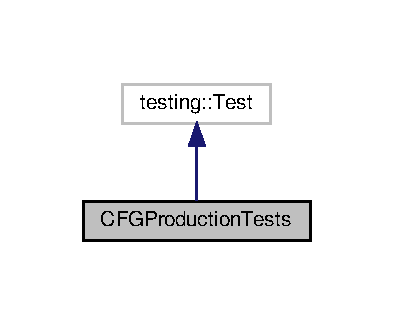
\includegraphics[width=189pt]{classCFGProductionTests__inherit__graph}
\end{center}
\end{figure}


Collaboration diagram for C\+F\+G\+Production\+Tests\+:
\nopagebreak
\begin{figure}[H]
\begin{center}
\leavevmode
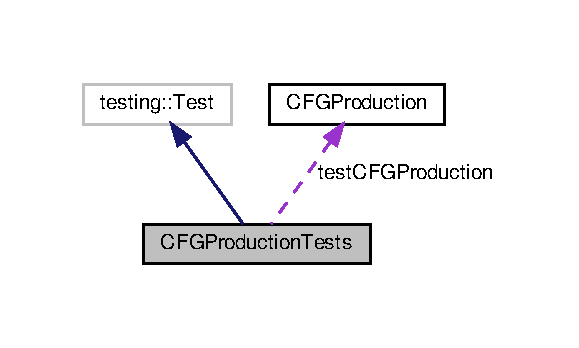
\includegraphics[width=278pt]{classCFGProductionTests__coll__graph}
\end{center}
\end{figure}
\subsection*{Protected Member Functions}
\begin{DoxyCompactItemize}
\item 
\mbox{\Hypertarget{classCFGProductionTests_ad140e7c490a16c0cb2cbf0a8f32a3c56}\label{classCFGProductionTests_ad140e7c490a16c0cb2cbf0a8f32a3c56}} 
virtual void {\bfseries Set\+Up} ()
\item 
\mbox{\Hypertarget{classCFGProductionTests_a5767daac7f43c05af1ff20f8c61b953c}\label{classCFGProductionTests_a5767daac7f43c05af1ff20f8c61b953c}} 
virtual void {\bfseries Tear\+Down} ()
\end{DoxyCompactItemize}
\subsection*{Protected Attributes}
\begin{DoxyCompactItemize}
\item 
\mbox{\Hypertarget{classCFGProductionTests_a58a043e77c5f16a08fc0e5d365141c8c}\label{classCFGProductionTests_a58a043e77c5f16a08fc0e5d365141c8c}} 
\hyperlink{classCFGProduction}{C\+F\+G\+Production} $\ast$ {\bfseries test\+C\+F\+G\+Production} = new \hyperlink{classCFGProduction}{C\+F\+G\+Production}()
\end{DoxyCompactItemize}


The documentation for this class was generated from the following file\+:\begin{DoxyCompactItemize}
\item 
Test/C\+F\+G\+Production\+Tests.\+cpp\end{DoxyCompactItemize}

\hypertarget{classCFGTests}{}\section{C\+F\+G\+Tests Class Reference}
\label{classCFGTests}\index{C\+F\+G\+Tests@{C\+F\+G\+Tests}}


Inheritance diagram for C\+F\+G\+Tests\+:
\nopagebreak
\begin{figure}[H]
\begin{center}
\leavevmode
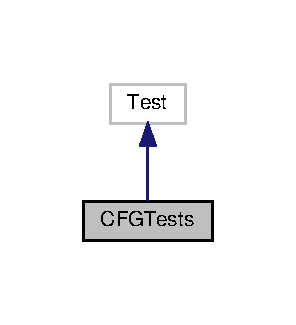
\includegraphics[width=142pt]{classCFGTests__inherit__graph}
\end{center}
\end{figure}


Collaboration diagram for C\+F\+G\+Tests\+:
\nopagebreak
\begin{figure}[H]
\begin{center}
\leavevmode
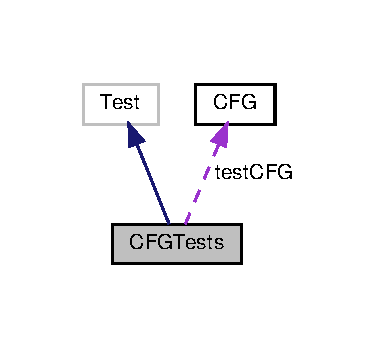
\includegraphics[width=181pt]{classCFGTests__coll__graph}
\end{center}
\end{figure}
\subsection*{Protected Member Functions}
\begin{DoxyCompactItemize}
\item 
\mbox{\Hypertarget{classCFGTests_ace2b5e18a5d98a8e8124f2f56fbd3b29}\label{classCFGTests_ace2b5e18a5d98a8e8124f2f56fbd3b29}} 
virtual void {\bfseries Set\+Up} ()
\item 
\mbox{\Hypertarget{classCFGTests_a01e25be05dfab8dad0184228fec480d9}\label{classCFGTests_a01e25be05dfab8dad0184228fec480d9}} 
virtual void {\bfseries Tear\+Down} ()
\end{DoxyCompactItemize}
\subsection*{Protected Attributes}
\begin{DoxyCompactItemize}
\item 
\mbox{\Hypertarget{classCFGTests_a630275f74118e1f25b0f4c1869a81f73}\label{classCFGTests_a630275f74118e1f25b0f4c1869a81f73}} 
\hyperlink{classCFG}{C\+FG} $\ast$ {\bfseries test\+C\+FG} = new \hyperlink{classCFG}{C\+FG}()
\end{DoxyCompactItemize}


The documentation for this class was generated from the following file\+:\begin{DoxyCompactItemize}
\item 
Test/C\+F\+G\+Tests.\+cpp\end{DoxyCompactItemize}

\hypertarget{structColor}{}\section{Color Struct Reference}
\label{structColor}\index{Color@{Color}}


This class represents the \hyperlink{structColor}{Color} in our logic system.  




{\ttfamily \#include $<$Game\+Object.\+h$>$}

\subsection*{Public Member Functions}
\begin{DoxyCompactItemize}
\item 
\hyperlink{structColor_a154354d16fc63294355979095a3b6d65}{Color} (int r, int g, int b)
\begin{DoxyCompactList}\small\item\em Constructor of \hyperlink{structColor}{Color} taking the R\+GB values. \end{DoxyCompactList}\item 
\mbox{\Hypertarget{structColor_a9a742cbe9f9f4037f5d9f4e81a9b2428}\label{structColor_a9a742cbe9f9f4037f5d9f4e81a9b2428}} 
\hyperlink{structColor_a9a742cbe9f9f4037f5d9f4e81a9b2428}{Color} ()
\begin{DoxyCompactList}\small\item\em Default constructor of \hyperlink{structColor}{Color}. \end{DoxyCompactList}\item 
\mbox{\Hypertarget{structColor_a3cfce6c6821d3bf489e26074c55378c0}\label{structColor_a3cfce6c6821d3bf489e26074c55378c0}} 
virtual \hyperlink{structColor_a3cfce6c6821d3bf489e26074c55378c0}{$\sim$\+Color} ()
\begin{DoxyCompactList}\small\item\em Default destructor. \end{DoxyCompactList}\end{DoxyCompactItemize}
\subsection*{Public Attributes}
\begin{DoxyCompactItemize}
\item 
\mbox{\Hypertarget{structColor_a4954bdc9772da2a610401b8a438125cb}\label{structColor_a4954bdc9772da2a610401b8a438125cb}} 
int {\bfseries r}
\item 
\mbox{\Hypertarget{structColor_ab5656e995bddd43d286c7ff5629a31dd}\label{structColor_ab5656e995bddd43d286c7ff5629a31dd}} 
int {\bfseries g}
\item 
\mbox{\Hypertarget{structColor_ae11f00d34bf3ecd8c8278f68876b82bf}\label{structColor_ae11f00d34bf3ecd8c8278f68876b82bf}} 
int {\bfseries b}
\end{DoxyCompactItemize}


\subsection{Detailed Description}
This class represents the \hyperlink{structColor}{Color} in our logic system. 

\subsection{Constructor \& Destructor Documentation}
\mbox{\Hypertarget{structColor_a154354d16fc63294355979095a3b6d65}\label{structColor_a154354d16fc63294355979095a3b6d65}} 
\index{Color@{Color}!Color@{Color}}
\index{Color@{Color}!Color@{Color}}
\subsubsection{\texorpdfstring{Color()}{Color()}}
{\footnotesize\ttfamily Color\+::\+Color (\begin{DoxyParamCaption}\item[{int}]{r,  }\item[{int}]{g,  }\item[{int}]{b }\end{DoxyParamCaption})}



Constructor of \hyperlink{structColor}{Color} taking the R\+GB values. 


\begin{DoxyParams}{Parameters}
{\em r} & Red value \\
\hline
{\em g} & Green value \\
\hline
{\em b} & Blue value \\
\hline
\end{DoxyParams}


The documentation for this struct was generated from the following files\+:\begin{DoxyCompactItemize}
\item 
include/Game\+Object.\+h\item 
src/Game\+Object.\+cpp\end{DoxyCompactItemize}

\hypertarget{classDtataSturctureTests}{}\section{Dtata\+Sturcture\+Tests Class Reference}
\label{classDtataSturctureTests}\index{Dtata\+Sturcture\+Tests@{Dtata\+Sturcture\+Tests}}


Inheritance diagram for Dtata\+Sturcture\+Tests\+:
\nopagebreak
\begin{figure}[H]
\begin{center}
\leavevmode
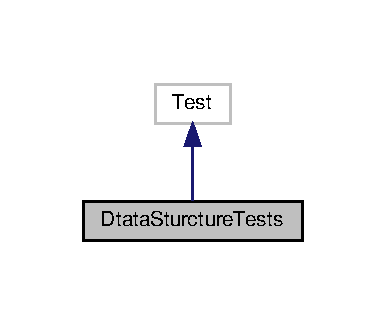
\includegraphics[width=185pt]{classDtataSturctureTests__inherit__graph}
\end{center}
\end{figure}


Collaboration diagram for Dtata\+Sturcture\+Tests\+:
\nopagebreak
\begin{figure}[H]
\begin{center}
\leavevmode
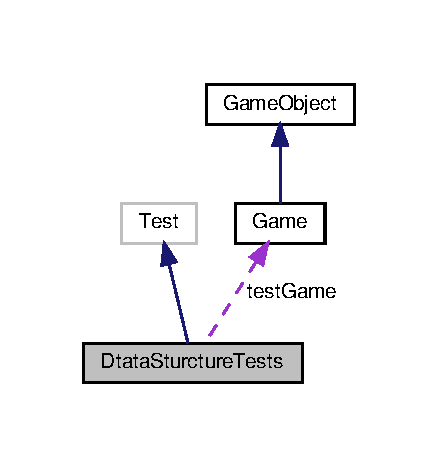
\includegraphics[width=210pt]{classDtataSturctureTests__coll__graph}
\end{center}
\end{figure}
\subsection*{Protected Member Functions}
\begin{DoxyCompactItemize}
\item 
\mbox{\Hypertarget{classDtataSturctureTests_a21ca6b840c86158f8ffe18d027589cfa}\label{classDtataSturctureTests_a21ca6b840c86158f8ffe18d027589cfa}} 
virtual void {\bfseries Set\+Up} ()
\item 
\mbox{\Hypertarget{classDtataSturctureTests_aa04d5e31252060e099c8fd1345becd90}\label{classDtataSturctureTests_aa04d5e31252060e099c8fd1345becd90}} 
virtual void {\bfseries Tear\+Down} ()
\end{DoxyCompactItemize}
\subsection*{Protected Attributes}
\begin{DoxyCompactItemize}
\item 
\mbox{\Hypertarget{classDtataSturctureTests_a6e6c4b1daf0275c60da92a16d2e16b2d}\label{classDtataSturctureTests_a6e6c4b1daf0275c60da92a16d2e16b2d}} 
\hyperlink{classGame}{Game} $\ast$ {\bfseries test\+Game} = new \hyperlink{classGame}{Game}()
\end{DoxyCompactItemize}


The documentation for this class was generated from the following file\+:\begin{DoxyCompactItemize}
\item 
Test/Data\+Structure\+Tests.\+cpp\end{DoxyCompactItemize}

\hypertarget{classEndObject}{}\section{End\+Object Class Reference}
\label{classEndObject}\index{End\+Object@{End\+Object}}


Inheritance diagram for End\+Object\+:
\nopagebreak
\begin{figure}[H]
\begin{center}
\leavevmode
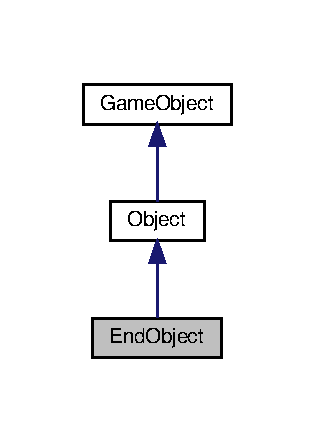
\includegraphics[width=151pt]{classEndObject__inherit__graph}
\end{center}
\end{figure}


Collaboration diagram for End\+Object\+:
\nopagebreak
\begin{figure}[H]
\begin{center}
\leavevmode
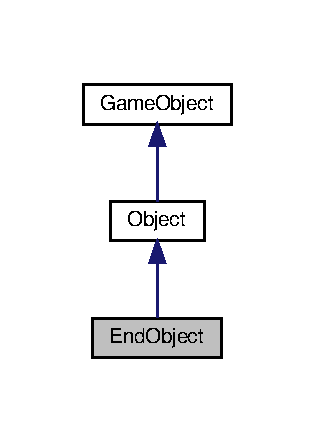
\includegraphics[width=151pt]{classEndObject__coll__graph}
\end{center}
\end{figure}
\subsection*{Public Member Functions}
\begin{DoxyCompactItemize}
\item 
\mbox{\Hypertarget{classEndObject_a3efa8c64e8a441d9a455cee8e0acf3cc}\label{classEndObject_a3efa8c64e8a441d9a455cee8e0acf3cc}} 
\hyperlink{classEndObject_a3efa8c64e8a441d9a455cee8e0acf3cc}{End\+Object} ()
\begin{DoxyCompactList}\small\item\em Default constructor of the end object class. \end{DoxyCompactList}\item 
\hyperlink{classEndObject_a2b7de61a785ee056d8ee82cb7e545b95}{End\+Object} (const std\+::string \&name)
\begin{DoxyCompactList}\small\item\em Constructor that takes the name of the End \hyperlink{classObject}{Object} as string. \end{DoxyCompactList}\item 
const string \& \hyperlink{classEndObject_a24ff73b898d1fa9fa15b98f490bf6bbc}{get\+Goto} () const
\begin{DoxyCompactList}\small\item\em returns where the endobject goes to \end{DoxyCompactList}\item 
void \hyperlink{classEndObject_af2fd8ca8246a6891f72f44aacd55cba4}{set\+Goto} (const string \&goto\+Obj)
\begin{DoxyCompactList}\small\item\em Sets the object where the end object goes to. \end{DoxyCompactList}\end{DoxyCompactItemize}


\subsection{Constructor \& Destructor Documentation}
\mbox{\Hypertarget{classEndObject_a2b7de61a785ee056d8ee82cb7e545b95}\label{classEndObject_a2b7de61a785ee056d8ee82cb7e545b95}} 
\index{End\+Object@{End\+Object}!End\+Object@{End\+Object}}
\index{End\+Object@{End\+Object}!End\+Object@{End\+Object}}
\subsubsection{\texorpdfstring{End\+Object()}{EndObject()}}
{\footnotesize\ttfamily End\+Object\+::\+End\+Object (\begin{DoxyParamCaption}\item[{const std\+::string \&}]{name }\end{DoxyParamCaption})\hspace{0.3cm}{\ttfamily [explicit]}}



Constructor that takes the name of the End \hyperlink{classObject}{Object} as string. 


\begin{DoxyParams}{Parameters}
{\em name} & Name of the End \hyperlink{classObject}{Object} \\
\hline
\end{DoxyParams}


\subsection{Member Function Documentation}
\mbox{\Hypertarget{classEndObject_a24ff73b898d1fa9fa15b98f490bf6bbc}\label{classEndObject_a24ff73b898d1fa9fa15b98f490bf6bbc}} 
\index{End\+Object@{End\+Object}!get\+Goto@{get\+Goto}}
\index{get\+Goto@{get\+Goto}!End\+Object@{End\+Object}}
\subsubsection{\texorpdfstring{get\+Goto()}{getGoto()}}
{\footnotesize\ttfamily const string \& End\+Object\+::get\+Goto (\begin{DoxyParamCaption}{ }\end{DoxyParamCaption}) const}



returns where the endobject goes to 

\begin{DoxyReturn}{Returns}
the string that is where the endobject goes to 
\end{DoxyReturn}
\mbox{\Hypertarget{classEndObject_af2fd8ca8246a6891f72f44aacd55cba4}\label{classEndObject_af2fd8ca8246a6891f72f44aacd55cba4}} 
\index{End\+Object@{End\+Object}!set\+Goto@{set\+Goto}}
\index{set\+Goto@{set\+Goto}!End\+Object@{End\+Object}}
\subsubsection{\texorpdfstring{set\+Goto()}{setGoto()}}
{\footnotesize\ttfamily void End\+Object\+::set\+Goto (\begin{DoxyParamCaption}\item[{const string \&}]{goto\+Obj }\end{DoxyParamCaption})}



Sets the object where the end object goes to. 


\begin{DoxyParams}{Parameters}
{\em goto\+Obj} & a string where the object is supposed to be going to \\
\hline
\end{DoxyParams}


The documentation for this class was generated from the following files\+:\begin{DoxyCompactItemize}
\item 
include/End\+Object.\+h\item 
src/End\+Object.\+cpp\end{DoxyCompactItemize}

\hypertarget{classEntity}{}\section{Entity Class Reference}
\label{classEntity}\index{Entity@{Entity}}


Class which represents an \hyperlink{classEntity}{Entity} of the \hyperlink{classGame}{Game} Derived from abstract \hyperlink{classGameObject}{Game\+Object}.  




{\ttfamily \#include $<$Entity.\+h$>$}



Inheritance diagram for Entity\+:
\nopagebreak
\begin{figure}[H]
\begin{center}
\leavevmode
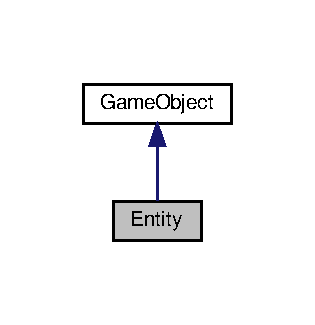
\includegraphics[width=151pt]{classEntity__inherit__graph}
\end{center}
\end{figure}


Collaboration diagram for Entity\+:
\nopagebreak
\begin{figure}[H]
\begin{center}
\leavevmode
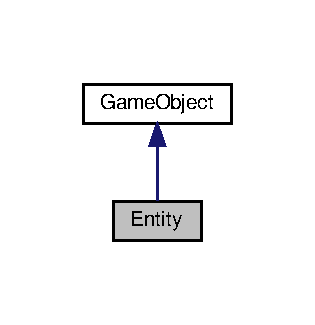
\includegraphics[width=151pt]{classEntity__coll__graph}
\end{center}
\end{figure}
\subsection*{Public Member Functions}
\begin{DoxyCompactItemize}
\item 
\hyperlink{classEntity_a0193c7a349273d65551c229ab1afabaf}{Entity} (int width, int height, double move\+Speed, double jump\+Height, const game\+Location \&location, const string \&m\+\_\+texture\+Path)
\begin{DoxyCompactList}\small\item\em Constructor for \hyperlink{classEntity}{Entity}. \end{DoxyCompactList}\item 
\mbox{\Hypertarget{classEntity_a980f368aa07ce358583982821533a54a}\label{classEntity_a980f368aa07ce358583982821533a54a}} 
\hyperlink{classEntity_a980f368aa07ce358583982821533a54a}{Entity} ()
\begin{DoxyCompactList}\small\item\em Default constructor for \hyperlink{classEntity}{Entity}. \end{DoxyCompactList}\item 
double \hyperlink{classEntity_ae702b415329b0c3f382747f0a6668115}{get\+Movement\+Speed} () const
\begin{DoxyCompactList}\small\item\em Getter for movement speed. \end{DoxyCompactList}\item 
double \hyperlink{classEntity_a4f950165af1db516a081d1085c21032e}{get\+Jump\+Height} () const
\begin{DoxyCompactList}\small\item\em Getter for jump height. \end{DoxyCompactList}\item 
const game\+Location \& \hyperlink{classEntity_a1096aa490b52f061d947b2cc3831266e}{get\+Location} () const
\begin{DoxyCompactList}\small\item\em Getter for the location of the entity. \end{DoxyCompactList}\item 
void \hyperlink{classEntity_ab6ccff5da8e3cdc67659b0e89158c199}{set\+Jump\+Height} (double jump\+Height)
\begin{DoxyCompactList}\small\item\em Setter for jump height. \end{DoxyCompactList}\item 
void \hyperlink{classEntity_a70bfcbab042dfd1f1571e06d406985f4}{set\+Location} (const game\+Location \&location)
\begin{DoxyCompactList}\small\item\em Setter for the location. \end{DoxyCompactList}\item 
void \hyperlink{classEntity_a1ee8abc607182bd4dc3a650cafb98188}{set\+Movement\+Speed} (double speed)
\begin{DoxyCompactList}\small\item\em Setter for movement speed of entity. \end{DoxyCompactList}\item 
\mbox{\Hypertarget{classEntity_a605d474ccbd30c3d4350016ec173546a}\label{classEntity_a605d474ccbd30c3d4350016ec173546a}} 
\hyperlink{classEntity_a605d474ccbd30c3d4350016ec173546a}{$\sim$\+Entity} () override=default
\begin{DoxyCompactList}\small\item\em Default destructor for \hyperlink{classEntity}{Entity}. \end{DoxyCompactList}\item 
virtual bool \hyperlink{classEntity_a01357a3f88d3d7277cff951fa1a63add}{is\+Player} () const
\begin{DoxyCompactList}\small\item\em Determine if the entity is a player or not. \end{DoxyCompactList}\item 
void \hyperlink{classEntity_ad80d65640fe9dd1ae0a0660f02dc60f5}{set\+Player\+Bool} (bool \hyperlink{classEntity_a01357a3f88d3d7277cff951fa1a63add}{is\+Player})
\begin{DoxyCompactList}\small\item\em Setter for bool to determine if entity is player or not. \end{DoxyCompactList}\end{DoxyCompactItemize}


\subsection{Detailed Description}
Class which represents an \hyperlink{classEntity}{Entity} of the \hyperlink{classGame}{Game} Derived from abstract \hyperlink{classGameObject}{Game\+Object}. 

\subsection{Constructor \& Destructor Documentation}
\mbox{\Hypertarget{classEntity_a0193c7a349273d65551c229ab1afabaf}\label{classEntity_a0193c7a349273d65551c229ab1afabaf}} 
\index{Entity@{Entity}!Entity@{Entity}}
\index{Entity@{Entity}!Entity@{Entity}}
\subsubsection{\texorpdfstring{Entity()}{Entity()}}
{\footnotesize\ttfamily Entity\+::\+Entity (\begin{DoxyParamCaption}\item[{int}]{width,  }\item[{int}]{height,  }\item[{double}]{move\+Speed,  }\item[{double}]{jump\+Height,  }\item[{const game\+Location \&}]{location,  }\item[{const string \&}]{m\+\_\+texture\+Path }\end{DoxyParamCaption})}



Constructor for \hyperlink{classEntity}{Entity}. 


\begin{DoxyParams}{Parameters}
{\em width} & Width of the entity \\
\hline
{\em height} & Height of the entity \\
\hline
{\em move\+Speed} & Movement speed of the entity \\
\hline
{\em jump\+Height} & Jump height of the entity \\
\hline
{\em location} & Location of the \hyperlink{classEntity}{Entity} \\
\hline
{\em m\+\_\+texture\+Path} & Path to texture of entity \\
\hline
\end{DoxyParams}


\subsection{Member Function Documentation}
\mbox{\Hypertarget{classEntity_a4f950165af1db516a081d1085c21032e}\label{classEntity_a4f950165af1db516a081d1085c21032e}} 
\index{Entity@{Entity}!get\+Jump\+Height@{get\+Jump\+Height}}
\index{get\+Jump\+Height@{get\+Jump\+Height}!Entity@{Entity}}
\subsubsection{\texorpdfstring{get\+Jump\+Height()}{getJumpHeight()}}
{\footnotesize\ttfamily double Entity\+::get\+Jump\+Height (\begin{DoxyParamCaption}{ }\end{DoxyParamCaption}) const}



Getter for jump height. 

\begin{DoxyReturn}{Returns}
Jump height (double) 
\end{DoxyReturn}
\mbox{\Hypertarget{classEntity_a1096aa490b52f061d947b2cc3831266e}\label{classEntity_a1096aa490b52f061d947b2cc3831266e}} 
\index{Entity@{Entity}!get\+Location@{get\+Location}}
\index{get\+Location@{get\+Location}!Entity@{Entity}}
\subsubsection{\texorpdfstring{get\+Location()}{getLocation()}}
{\footnotesize\ttfamily const game\+Location \& Entity\+::get\+Location (\begin{DoxyParamCaption}{ }\end{DoxyParamCaption}) const}



Getter for the location of the entity. 

\begin{DoxyReturn}{Returns}
Location of the entity 
\end{DoxyReturn}
\mbox{\Hypertarget{classEntity_ae702b415329b0c3f382747f0a6668115}\label{classEntity_ae702b415329b0c3f382747f0a6668115}} 
\index{Entity@{Entity}!get\+Movement\+Speed@{get\+Movement\+Speed}}
\index{get\+Movement\+Speed@{get\+Movement\+Speed}!Entity@{Entity}}
\subsubsection{\texorpdfstring{get\+Movement\+Speed()}{getMovementSpeed()}}
{\footnotesize\ttfamily double Entity\+::get\+Movement\+Speed (\begin{DoxyParamCaption}{ }\end{DoxyParamCaption}) const}



Getter for movement speed. 

\begin{DoxyReturn}{Returns}
Movement speed (double) 
\end{DoxyReturn}
\mbox{\Hypertarget{classEntity_a01357a3f88d3d7277cff951fa1a63add}\label{classEntity_a01357a3f88d3d7277cff951fa1a63add}} 
\index{Entity@{Entity}!is\+Player@{is\+Player}}
\index{is\+Player@{is\+Player}!Entity@{Entity}}
\subsubsection{\texorpdfstring{is\+Player()}{isPlayer()}}
{\footnotesize\ttfamily bool Entity\+::is\+Player (\begin{DoxyParamCaption}{ }\end{DoxyParamCaption}) const\hspace{0.3cm}{\ttfamily [virtual]}}



Determine if the entity is a player or not. 

\begin{DoxyReturn}{Returns}
True if the entity is a player 
\end{DoxyReturn}
\mbox{\Hypertarget{classEntity_ab6ccff5da8e3cdc67659b0e89158c199}\label{classEntity_ab6ccff5da8e3cdc67659b0e89158c199}} 
\index{Entity@{Entity}!set\+Jump\+Height@{set\+Jump\+Height}}
\index{set\+Jump\+Height@{set\+Jump\+Height}!Entity@{Entity}}
\subsubsection{\texorpdfstring{set\+Jump\+Height()}{setJumpHeight()}}
{\footnotesize\ttfamily void Entity\+::set\+Jump\+Height (\begin{DoxyParamCaption}\item[{double}]{jump\+Height }\end{DoxyParamCaption})}



Setter for jump height. 


\begin{DoxyParams}{Parameters}
{\em jump\+Height} & Jump height of the entity \\
\hline
\end{DoxyParams}
\mbox{\Hypertarget{classEntity_a70bfcbab042dfd1f1571e06d406985f4}\label{classEntity_a70bfcbab042dfd1f1571e06d406985f4}} 
\index{Entity@{Entity}!set\+Location@{set\+Location}}
\index{set\+Location@{set\+Location}!Entity@{Entity}}
\subsubsection{\texorpdfstring{set\+Location()}{setLocation()}}
{\footnotesize\ttfamily void Entity\+::set\+Location (\begin{DoxyParamCaption}\item[{const game\+Location \&}]{location }\end{DoxyParamCaption})}



Setter for the location. 


\begin{DoxyParams}{Parameters}
{\em location} & Location of the entity \\
\hline
\end{DoxyParams}
\mbox{\Hypertarget{classEntity_a1ee8abc607182bd4dc3a650cafb98188}\label{classEntity_a1ee8abc607182bd4dc3a650cafb98188}} 
\index{Entity@{Entity}!set\+Movement\+Speed@{set\+Movement\+Speed}}
\index{set\+Movement\+Speed@{set\+Movement\+Speed}!Entity@{Entity}}
\subsubsection{\texorpdfstring{set\+Movement\+Speed()}{setMovementSpeed()}}
{\footnotesize\ttfamily void Entity\+::set\+Movement\+Speed (\begin{DoxyParamCaption}\item[{double}]{speed }\end{DoxyParamCaption})}



Setter for movement speed of entity. 


\begin{DoxyParams}{Parameters}
{\em speed} & Movement speed of entity \\
\hline
\end{DoxyParams}
\mbox{\Hypertarget{classEntity_ad80d65640fe9dd1ae0a0660f02dc60f5}\label{classEntity_ad80d65640fe9dd1ae0a0660f02dc60f5}} 
\index{Entity@{Entity}!set\+Player\+Bool@{set\+Player\+Bool}}
\index{set\+Player\+Bool@{set\+Player\+Bool}!Entity@{Entity}}
\subsubsection{\texorpdfstring{set\+Player\+Bool()}{setPlayerBool()}}
{\footnotesize\ttfamily void Entity\+::set\+Player\+Bool (\begin{DoxyParamCaption}\item[{bool}]{is\+Player }\end{DoxyParamCaption})}



Setter for bool to determine if entity is player or not. 


\begin{DoxyParams}{Parameters}
{\em is\+Player} & Bool which identifies the player \\
\hline
\end{DoxyParams}


The documentation for this class was generated from the following files\+:\begin{DoxyCompactItemize}
\item 
include/Entity.\+h\item 
src/Entity.\+cpp\end{DoxyCompactItemize}

\hypertarget{classGame}{}\section{Game Class Reference}
\label{classGame}\index{Game@{Game}}


This class is the container of the game.  




{\ttfamily \#include $<$Game.\+h$>$}



Inheritance diagram for Game\+:
\nopagebreak
\begin{figure}[H]
\begin{center}
\leavevmode
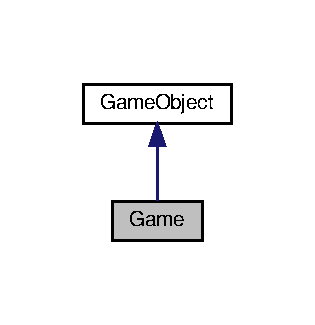
\includegraphics[width=151pt]{classGame__inherit__graph}
\end{center}
\end{figure}


Collaboration diagram for Game\+:
\nopagebreak
\begin{figure}[H]
\begin{center}
\leavevmode
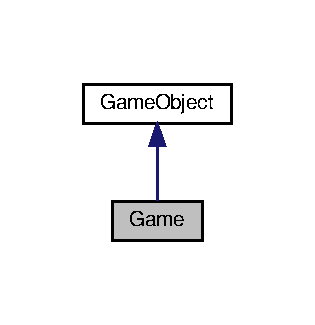
\includegraphics[width=151pt]{classGame__coll__graph}
\end{center}
\end{figure}
\subsection*{Public Member Functions}
\begin{DoxyCompactItemize}
\item 
\mbox{\Hypertarget{classGame_a4735989677c1cab18866f3ae4ee0aa1c}\label{classGame_a4735989677c1cab18866f3ae4ee0aa1c}} 
\hyperlink{classGame_a4735989677c1cab18866f3ae4ee0aa1c}{Game} ()=default
\begin{DoxyCompactList}\small\item\em Default constructor for the game. \end{DoxyCompactList}\item 
\hyperlink{classGame_a390a5384cd8ed6839148d036499b2d95}{Game} (const std\+::string \&game\+Name)
\begin{DoxyCompactList}\small\item\em Constructor of the game that takes the name of the game as inut. \end{DoxyCompactList}\item 
void \hyperlink{classGame_aa85c4d8154aff77cd064b859ea6c1da2}{add\+Level} (shared\+\_\+ptr$<$ \hyperlink{classLevel}{Level} $>$ level)
\begin{DoxyCompactList}\small\item\em Adds a level to the game. \end{DoxyCompactList}\item 
void \hyperlink{classGame_ad130d02a37e7754ff619d8b28c5d52ea}{set\+Levels} (const vector$<$ shared\+\_\+ptr$<$ \hyperlink{classLevel}{Level} $>$$>$ \&levels)
\begin{DoxyCompactList}\small\item\em Sets the levels of the game. \end{DoxyCompactList}\item 
const vector$<$ shared\+\_\+ptr$<$ \hyperlink{classLevel}{Level} $>$ $>$ \& \hyperlink{classGame_a7054929dc897593d0d5bace74398df9b}{get\+Levels} () const
\begin{DoxyCompactList}\small\item\em Returns a level. \end{DoxyCompactList}\item 
\mbox{\Hypertarget{classGame_a09ffcdf9d805fd9a407f68865661373d}\label{classGame_a09ffcdf9d805fd9a407f68865661373d}} 
\hyperlink{classGame_a09ffcdf9d805fd9a407f68865661373d}{$\sim$\+Game} () override=default
\begin{DoxyCompactList}\small\item\em default destructor \end{DoxyCompactList}\end{DoxyCompactItemize}


\subsection{Detailed Description}
This class is the container of the game. 

\subsection{Constructor \& Destructor Documentation}
\mbox{\Hypertarget{classGame_a390a5384cd8ed6839148d036499b2d95}\label{classGame_a390a5384cd8ed6839148d036499b2d95}} 
\index{Game@{Game}!Game@{Game}}
\index{Game@{Game}!Game@{Game}}
\subsubsection{\texorpdfstring{Game()}{Game()}}
{\footnotesize\ttfamily Game\+::\+Game (\begin{DoxyParamCaption}\item[{const std\+::string \&}]{game\+Name }\end{DoxyParamCaption})\hspace{0.3cm}{\ttfamily [explicit]}}



Constructor of the game that takes the name of the game as inut. 


\begin{DoxyParams}{Parameters}
{\em game\+Name} & String that is the name of the game \\
\hline
\end{DoxyParams}


\subsection{Member Function Documentation}
\mbox{\Hypertarget{classGame_aa85c4d8154aff77cd064b859ea6c1da2}\label{classGame_aa85c4d8154aff77cd064b859ea6c1da2}} 
\index{Game@{Game}!add\+Level@{add\+Level}}
\index{add\+Level@{add\+Level}!Game@{Game}}
\subsubsection{\texorpdfstring{add\+Level()}{addLevel()}}
{\footnotesize\ttfamily void Game\+::add\+Level (\begin{DoxyParamCaption}\item[{shared\+\_\+ptr$<$ \hyperlink{classLevel}{Level} $>$}]{level }\end{DoxyParamCaption})}



Adds a level to the game. 


\begin{DoxyParams}{Parameters}
{\em level} & a pointer to a new level \\
\hline
\end{DoxyParams}
\mbox{\Hypertarget{classGame_a7054929dc897593d0d5bace74398df9b}\label{classGame_a7054929dc897593d0d5bace74398df9b}} 
\index{Game@{Game}!get\+Levels@{get\+Levels}}
\index{get\+Levels@{get\+Levels}!Game@{Game}}
\subsubsection{\texorpdfstring{get\+Levels()}{getLevels()}}
{\footnotesize\ttfamily const vector$<$ shared\+\_\+ptr$<$ \hyperlink{classLevel}{Level} $>$ $>$ \& Game\+::get\+Levels (\begin{DoxyParamCaption}{ }\end{DoxyParamCaption}) const}



Returns a level. 

\begin{DoxyReturn}{Returns}
a shared pointer to the levels 
\end{DoxyReturn}
\mbox{\Hypertarget{classGame_ad130d02a37e7754ff619d8b28c5d52ea}\label{classGame_ad130d02a37e7754ff619d8b28c5d52ea}} 
\index{Game@{Game}!set\+Levels@{set\+Levels}}
\index{set\+Levels@{set\+Levels}!Game@{Game}}
\subsubsection{\texorpdfstring{set\+Levels()}{setLevels()}}
{\footnotesize\ttfamily void Game\+::set\+Levels (\begin{DoxyParamCaption}\item[{const vector$<$ shared\+\_\+ptr$<$ \hyperlink{classLevel}{Level} $>$$>$ \&}]{levels }\end{DoxyParamCaption})}



Sets the levels of the game. 


\begin{DoxyParams}{Parameters}
{\em levels} & a shared pointer to the levels \\
\hline
\end{DoxyParams}


The documentation for this class was generated from the following files\+:\begin{DoxyCompactItemize}
\item 
include/Game.\+h\item 
src/Game.\+cpp\end{DoxyCompactItemize}

\hypertarget{classGameObject}{}\section{Game\+Object Class Reference}
\label{classGameObject}\index{Game\+Object@{Game\+Object}}


Abstract class for each game object.  




{\ttfamily \#include $<$Game\+Object.\+h$>$}



Inheritance diagram for Game\+Object\+:
\nopagebreak
\begin{figure}[H]
\begin{center}
\leavevmode
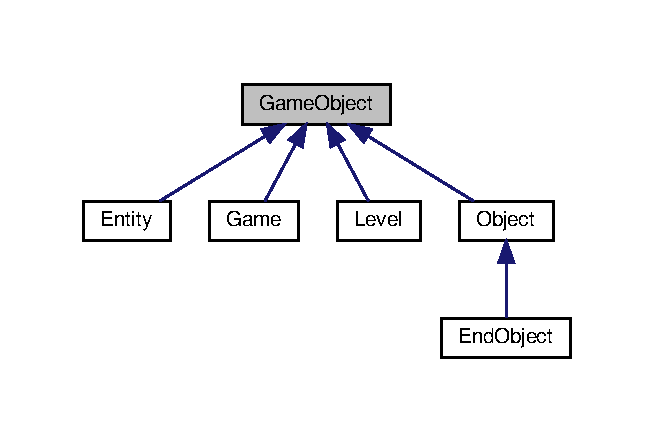
\includegraphics[width=314pt]{classGameObject__inherit__graph}
\end{center}
\end{figure}
\subsection*{Public Member Functions}
\begin{DoxyCompactItemize}
\item 
\mbox{\Hypertarget{classGameObject_a0348e3ee2e83d56eafca7a3547f432c4}\label{classGameObject_a0348e3ee2e83d56eafca7a3547f432c4}} 
\hyperlink{classGameObject_a0348e3ee2e83d56eafca7a3547f432c4}{Game\+Object} ()
\begin{DoxyCompactList}\small\item\em Default constructor. \end{DoxyCompactList}\item 
\hyperlink{classGameObject_af1571c09945131e1d791dfbbe56d69df}{Game\+Object} (int width, int height)
\begin{DoxyCompactList}\small\item\em Constructor of game object. \end{DoxyCompactList}\item 
\hyperlink{classGameObject_ae18349131123d744c2f0e89114272b38}{Game\+Object} (int width, int height, std\+::shared\+\_\+ptr$<$ \hyperlink{structColor}{Color} $>$ color)
\begin{DoxyCompactList}\small\item\em Constructor of game object with color. \end{DoxyCompactList}\item 
int \hyperlink{classGameObject_a912dd50a89fa0ea4bb674ece6fd993a4}{get\+Width} () const
\begin{DoxyCompactList}\small\item\em Getter of the width. \end{DoxyCompactList}\item 
void \hyperlink{classGameObject_aea1d6398e4b66af6987c24e7728463ad}{set\+Width} (int width)
\begin{DoxyCompactList}\small\item\em Setter of the width. \end{DoxyCompactList}\item 
int \hyperlink{classGameObject_a6aac91785cfba6631668db216235c79e}{get\+Height} () const
\begin{DoxyCompactList}\small\item\em Getter of the height. \end{DoxyCompactList}\item 
void \hyperlink{classGameObject_aa08869921287057b06c7f2ae89eef9ab}{set\+Height} (int height)
\begin{DoxyCompactList}\small\item\em sets the height \end{DoxyCompactList}\item 
const std\+::shared\+\_\+ptr$<$ \hyperlink{structColor}{Color} $>$ \& \hyperlink{classGameObject_aa51b4277277c1c851e59847015c937e8}{get\+Color} () const
\begin{DoxyCompactList}\small\item\em Getter of the color. \end{DoxyCompactList}\item 
void \hyperlink{classGameObject_a9751f8cfc3a86b61524879fb3f0aea79}{set\+Color} (const std\+::shared\+\_\+ptr$<$ \hyperlink{structColor}{Color} $>$ \&color)
\begin{DoxyCompactList}\small\item\em Setter of the color. \end{DoxyCompactList}\item 
void \hyperlink{classGameObject_a728c8a03416fd7bde2498d79ae6c26a3}{set\+Name} (const std\+::string \&name)
\begin{DoxyCompactList}\small\item\em Sets the name of the game object. \end{DoxyCompactList}\item 
const std\+::string \& \hyperlink{classGameObject_a72c04187da1840a922b7cbafa12e4882}{get\+Name} () const
\begin{DoxyCompactList}\small\item\em Returns the gamename. \end{DoxyCompactList}\item 
\mbox{\Hypertarget{classGameObject_a67ae2fa6e7916c799700cd659975d8ea}\label{classGameObject_a67ae2fa6e7916c799700cd659975d8ea}} 
virtual \hyperlink{classGameObject_a67ae2fa6e7916c799700cd659975d8ea}{$\sim$\+Game\+Object} ()=default
\begin{DoxyCompactList}\small\item\em default destructor \end{DoxyCompactList}\item 
const string \& \hyperlink{classGameObject_a008037b2f4572fe79d38d5abea5b1058}{get\+Texture\+Path} () const
\begin{DoxyCompactList}\small\item\em Getter for the Texture path of the object. \end{DoxyCompactList}\item 
void \hyperlink{classGameObject_a0d9759f01e8098149ce3e69cb8878534}{set\+Texture\+Path} (const string \&texture\+Path)
\begin{DoxyCompactList}\small\item\em Setter for texture path of the object. \end{DoxyCompactList}\item 
bool \hyperlink{classGameObject_a70e86ba6707ed1b23bb37d1336cd41df}{has\+Texture} () const
\begin{DoxyCompactList}\small\item\em Determine whether a \hyperlink{classGameObject}{Game\+Object} has a texture or not. \end{DoxyCompactList}\item 
void \hyperlink{classGameObject_a47616d924a30ae7db22387234c0381a1}{scale} (float scaleX, float scaleY)
\begin{DoxyCompactList}\small\item\em Scales the \hyperlink{classGameObject}{Game\+Object} that must be drawn correctly. \end{DoxyCompactList}\item 
\mbox{\Hypertarget{classGameObject_a3db3881d7943862b683cda0c08439a63}\label{classGameObject_a3db3881d7943862b683cda0c08439a63}} 
void {\bfseries set\+Position} (const game\+Location \&location)
\item 
\mbox{\Hypertarget{classGameObject_abf4de46e52c8f23d18d51bc29744b136}\label{classGameObject_abf4de46e52c8f23d18d51bc29744b136}} 
void {\bfseries draw} (sf\+::\+Render\+Window \&window)
\end{DoxyCompactItemize}


\subsection{Detailed Description}
Abstract class for each game object. 

\subsection{Constructor \& Destructor Documentation}
\mbox{\Hypertarget{classGameObject_af1571c09945131e1d791dfbbe56d69df}\label{classGameObject_af1571c09945131e1d791dfbbe56d69df}} 
\index{Game\+Object@{Game\+Object}!Game\+Object@{Game\+Object}}
\index{Game\+Object@{Game\+Object}!Game\+Object@{Game\+Object}}
\subsubsection{\texorpdfstring{Game\+Object()}{GameObject()}\hspace{0.1cm}{\footnotesize\ttfamily [1/2]}}
{\footnotesize\ttfamily Game\+Object\+::\+Game\+Object (\begin{DoxyParamCaption}\item[{int}]{width,  }\item[{int}]{height }\end{DoxyParamCaption})}



Constructor of game object. 


\begin{DoxyParams}{Parameters}
{\em width} & The width of the game object \\
\hline
{\em height} & The height of the game object \\
\hline
\end{DoxyParams}
\mbox{\Hypertarget{classGameObject_ae18349131123d744c2f0e89114272b38}\label{classGameObject_ae18349131123d744c2f0e89114272b38}} 
\index{Game\+Object@{Game\+Object}!Game\+Object@{Game\+Object}}
\index{Game\+Object@{Game\+Object}!Game\+Object@{Game\+Object}}
\subsubsection{\texorpdfstring{Game\+Object()}{GameObject()}\hspace{0.1cm}{\footnotesize\ttfamily [2/2]}}
{\footnotesize\ttfamily Game\+Object\+::\+Game\+Object (\begin{DoxyParamCaption}\item[{int}]{width,  }\item[{int}]{height,  }\item[{std\+::shared\+\_\+ptr$<$ \hyperlink{structColor}{Color} $>$}]{color }\end{DoxyParamCaption})}



Constructor of game object with color. 


\begin{DoxyParams}{Parameters}
{\em width} & Width of the game object \\
\hline
{\em height} & Height of the game object \\
\hline
{\em color} & \hyperlink{structColor}{Color} of the game object \\
\hline
\end{DoxyParams}


\subsection{Member Function Documentation}
\mbox{\Hypertarget{classGameObject_aa51b4277277c1c851e59847015c937e8}\label{classGameObject_aa51b4277277c1c851e59847015c937e8}} 
\index{Game\+Object@{Game\+Object}!get\+Color@{get\+Color}}
\index{get\+Color@{get\+Color}!Game\+Object@{Game\+Object}}
\subsubsection{\texorpdfstring{get\+Color()}{getColor()}}
{\footnotesize\ttfamily const std\+::shared\+\_\+ptr$<$ \hyperlink{structColor}{Color} $>$ \& Game\+Object\+::get\+Color (\begin{DoxyParamCaption}{ }\end{DoxyParamCaption}) const}



Getter of the color. 

\begin{DoxyReturn}{Returns}
Shared pointer that is the color 
\end{DoxyReturn}
\mbox{\Hypertarget{classGameObject_a6aac91785cfba6631668db216235c79e}\label{classGameObject_a6aac91785cfba6631668db216235c79e}} 
\index{Game\+Object@{Game\+Object}!get\+Height@{get\+Height}}
\index{get\+Height@{get\+Height}!Game\+Object@{Game\+Object}}
\subsubsection{\texorpdfstring{get\+Height()}{getHeight()}}
{\footnotesize\ttfamily int Game\+Object\+::get\+Height (\begin{DoxyParamCaption}{ }\end{DoxyParamCaption}) const}



Getter of the height. 

\begin{DoxyReturn}{Returns}
int, height 
\end{DoxyReturn}
\mbox{\Hypertarget{classGameObject_a72c04187da1840a922b7cbafa12e4882}\label{classGameObject_a72c04187da1840a922b7cbafa12e4882}} 
\index{Game\+Object@{Game\+Object}!get\+Name@{get\+Name}}
\index{get\+Name@{get\+Name}!Game\+Object@{Game\+Object}}
\subsubsection{\texorpdfstring{get\+Name()}{getName()}}
{\footnotesize\ttfamily const std\+::string \& Game\+Object\+::get\+Name (\begin{DoxyParamCaption}{ }\end{DoxyParamCaption}) const}



Returns the gamename. 

\begin{DoxyReturn}{Returns}
The name of the game 
\end{DoxyReturn}
\mbox{\Hypertarget{classGameObject_a008037b2f4572fe79d38d5abea5b1058}\label{classGameObject_a008037b2f4572fe79d38d5abea5b1058}} 
\index{Game\+Object@{Game\+Object}!get\+Texture\+Path@{get\+Texture\+Path}}
\index{get\+Texture\+Path@{get\+Texture\+Path}!Game\+Object@{Game\+Object}}
\subsubsection{\texorpdfstring{get\+Texture\+Path()}{getTexturePath()}}
{\footnotesize\ttfamily const string \& Game\+Object\+::get\+Texture\+Path (\begin{DoxyParamCaption}{ }\end{DoxyParamCaption}) const}



Getter for the Texture path of the object. 

\begin{DoxyReturn}{Returns}
String which represents texture path 
\end{DoxyReturn}
\mbox{\Hypertarget{classGameObject_a912dd50a89fa0ea4bb674ece6fd993a4}\label{classGameObject_a912dd50a89fa0ea4bb674ece6fd993a4}} 
\index{Game\+Object@{Game\+Object}!get\+Width@{get\+Width}}
\index{get\+Width@{get\+Width}!Game\+Object@{Game\+Object}}
\subsubsection{\texorpdfstring{get\+Width()}{getWidth()}}
{\footnotesize\ttfamily int Game\+Object\+::get\+Width (\begin{DoxyParamCaption}{ }\end{DoxyParamCaption}) const}



Getter of the width. 

\begin{DoxyReturn}{Returns}
int, width 
\end{DoxyReturn}
\mbox{\Hypertarget{classGameObject_a70e86ba6707ed1b23bb37d1336cd41df}\label{classGameObject_a70e86ba6707ed1b23bb37d1336cd41df}} 
\index{Game\+Object@{Game\+Object}!has\+Texture@{has\+Texture}}
\index{has\+Texture@{has\+Texture}!Game\+Object@{Game\+Object}}
\subsubsection{\texorpdfstring{has\+Texture()}{hasTexture()}}
{\footnotesize\ttfamily bool Game\+Object\+::has\+Texture (\begin{DoxyParamCaption}{ }\end{DoxyParamCaption}) const}



Determine whether a \hyperlink{classGameObject}{Game\+Object} has a texture or not. 

\begin{DoxyReturn}{Returns}
True if the \hyperlink{classGameObject}{Game\+Object} has a texture. 
\end{DoxyReturn}
\mbox{\Hypertarget{classGameObject_a47616d924a30ae7db22387234c0381a1}\label{classGameObject_a47616d924a30ae7db22387234c0381a1}} 
\index{Game\+Object@{Game\+Object}!scale@{scale}}
\index{scale@{scale}!Game\+Object@{Game\+Object}}
\subsubsection{\texorpdfstring{scale()}{scale()}}
{\footnotesize\ttfamily void Game\+Object\+::scale (\begin{DoxyParamCaption}\item[{float}]{scaleX,  }\item[{float}]{scaleY }\end{DoxyParamCaption})}



Scales the \hyperlink{classGameObject}{Game\+Object} that must be drawn correctly. 

If the \hyperlink{classGameObject}{Game\+Object} has a texture, the sprite will be scaled, else the rectangle will be scaled. 
\begin{DoxyParams}{Parameters}
{\em scaleX} & Scale factor of X. \\
\hline
{\em scaleY} & Scale factor of Y. \\
\hline
\end{DoxyParams}
\mbox{\Hypertarget{classGameObject_a9751f8cfc3a86b61524879fb3f0aea79}\label{classGameObject_a9751f8cfc3a86b61524879fb3f0aea79}} 
\index{Game\+Object@{Game\+Object}!set\+Color@{set\+Color}}
\index{set\+Color@{set\+Color}!Game\+Object@{Game\+Object}}
\subsubsection{\texorpdfstring{set\+Color()}{setColor()}}
{\footnotesize\ttfamily void Game\+Object\+::set\+Color (\begin{DoxyParamCaption}\item[{const std\+::shared\+\_\+ptr$<$ \hyperlink{structColor}{Color} $>$ \&}]{color }\end{DoxyParamCaption})}



Setter of the color. 


\begin{DoxyParams}{Parameters}
{\em color} & A shared pointer that is the color \\
\hline
\end{DoxyParams}
\mbox{\Hypertarget{classGameObject_aa08869921287057b06c7f2ae89eef9ab}\label{classGameObject_aa08869921287057b06c7f2ae89eef9ab}} 
\index{Game\+Object@{Game\+Object}!set\+Height@{set\+Height}}
\index{set\+Height@{set\+Height}!Game\+Object@{Game\+Object}}
\subsubsection{\texorpdfstring{set\+Height()}{setHeight()}}
{\footnotesize\ttfamily void Game\+Object\+::set\+Height (\begin{DoxyParamCaption}\item[{int}]{height }\end{DoxyParamCaption})}



sets the height 


\begin{DoxyParams}{Parameters}
{\em height} & An int that is supposed to be the height \\
\hline
\end{DoxyParams}
\mbox{\Hypertarget{classGameObject_a728c8a03416fd7bde2498d79ae6c26a3}\label{classGameObject_a728c8a03416fd7bde2498d79ae6c26a3}} 
\index{Game\+Object@{Game\+Object}!set\+Name@{set\+Name}}
\index{set\+Name@{set\+Name}!Game\+Object@{Game\+Object}}
\subsubsection{\texorpdfstring{set\+Name()}{setName()}}
{\footnotesize\ttfamily void Game\+Object\+::set\+Name (\begin{DoxyParamCaption}\item[{const std\+::string \&}]{name }\end{DoxyParamCaption})}



Sets the name of the game object. 


\begin{DoxyParams}{Parameters}
{\em name} & The string that is the name \\
\hline
\end{DoxyParams}
\mbox{\Hypertarget{classGameObject_a0d9759f01e8098149ce3e69cb8878534}\label{classGameObject_a0d9759f01e8098149ce3e69cb8878534}} 
\index{Game\+Object@{Game\+Object}!set\+Texture\+Path@{set\+Texture\+Path}}
\index{set\+Texture\+Path@{set\+Texture\+Path}!Game\+Object@{Game\+Object}}
\subsubsection{\texorpdfstring{set\+Texture\+Path()}{setTexturePath()}}
{\footnotesize\ttfamily void Game\+Object\+::set\+Texture\+Path (\begin{DoxyParamCaption}\item[{const string \&}]{texture\+Path }\end{DoxyParamCaption})}



Setter for texture path of the object. 

Also check if the texture can be loaded, and loads it into m\+\_\+texture if possible. If the texture is loaded, the sprite will be initialized. 
\begin{DoxyParams}{Parameters}
{\em texture\+Path} & Texture path of the object\\
\hline
{\em texture\+Path} & Texture path of the object \\
\hline
\end{DoxyParams}
\mbox{\Hypertarget{classGameObject_aea1d6398e4b66af6987c24e7728463ad}\label{classGameObject_aea1d6398e4b66af6987c24e7728463ad}} 
\index{Game\+Object@{Game\+Object}!set\+Width@{set\+Width}}
\index{set\+Width@{set\+Width}!Game\+Object@{Game\+Object}}
\subsubsection{\texorpdfstring{set\+Width()}{setWidth()}}
{\footnotesize\ttfamily void Game\+Object\+::set\+Width (\begin{DoxyParamCaption}\item[{int}]{width }\end{DoxyParamCaption})}



Setter of the width. 


\begin{DoxyParams}{Parameters}
{\em width} & The int that is supposed to be the width \\
\hline
\end{DoxyParams}


The documentation for this class was generated from the following files\+:\begin{DoxyCompactItemize}
\item 
include/Game\+Object.\+h\item 
src/Game\+Object.\+cpp\end{DoxyCompactItemize}

\hypertarget{classGameTests}{}\section{Game\+Tests Class Reference}
\label{classGameTests}\index{Game\+Tests@{Game\+Tests}}


Inheritance diagram for Game\+Tests\+:
\nopagebreak
\begin{figure}[H]
\begin{center}
\leavevmode
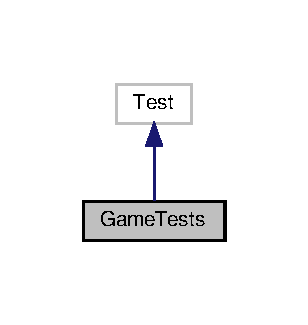
\includegraphics[width=148pt]{classGameTests__inherit__graph}
\end{center}
\end{figure}


Collaboration diagram for Game\+Tests\+:
\nopagebreak
\begin{figure}[H]
\begin{center}
\leavevmode
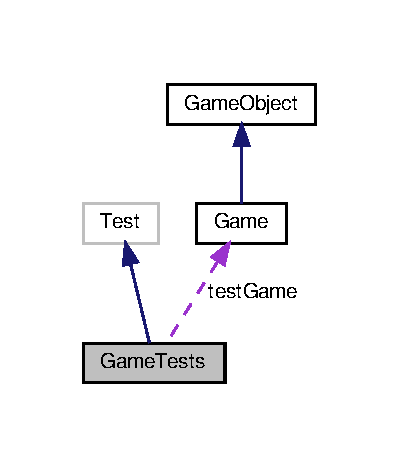
\includegraphics[width=192pt]{classGameTests__coll__graph}
\end{center}
\end{figure}
\subsection*{Protected Member Functions}
\begin{DoxyCompactItemize}
\item 
\mbox{\Hypertarget{classGameTests_a26d16cb8feeac7e3093df07905e2585e}\label{classGameTests_a26d16cb8feeac7e3093df07905e2585e}} 
virtual void {\bfseries Set\+Up} ()
\item 
\mbox{\Hypertarget{classGameTests_a028fd3fe94c168d98c6b284d04613f0c}\label{classGameTests_a028fd3fe94c168d98c6b284d04613f0c}} 
virtual void {\bfseries Tear\+Down} ()
\end{DoxyCompactItemize}
\subsection*{Protected Attributes}
\begin{DoxyCompactItemize}
\item 
\mbox{\Hypertarget{classGameTests_a63436947b204dc10220003394490be41}\label{classGameTests_a63436947b204dc10220003394490be41}} 
\hyperlink{classGame}{Game} $\ast$ {\bfseries test\+Game} = new \hyperlink{classGame}{Game}()
\end{DoxyCompactItemize}


The documentation for this class was generated from the following file\+:\begin{DoxyCompactItemize}
\item 
Test/Game\+Tests.\+cpp\end{DoxyCompactItemize}

\hypertarget{classLevel}{}\section{Level Class Reference}
\label{classLevel}\index{Level@{Level}}


Represents a level of the game.  




{\ttfamily \#include $<$Level.\+h$>$}



Inheritance diagram for Level\+:
\nopagebreak
\begin{figure}[H]
\begin{center}
\leavevmode
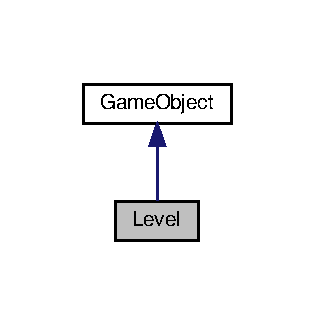
\includegraphics[width=151pt]{classLevel__inherit__graph}
\end{center}
\end{figure}


Collaboration diagram for Level\+:
\nopagebreak
\begin{figure}[H]
\begin{center}
\leavevmode
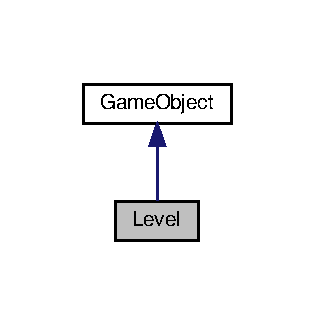
\includegraphics[width=151pt]{classLevel__coll__graph}
\end{center}
\end{figure}
\subsection*{Public Member Functions}
\begin{DoxyCompactItemize}
\item 
\mbox{\Hypertarget{classLevel_a7a696c928ca5d5354db6e50e46d0f67d}\label{classLevel_a7a696c928ca5d5354db6e50e46d0f67d}} 
\hyperlink{classLevel_a7a696c928ca5d5354db6e50e46d0f67d}{Level} ()
\begin{DoxyCompactList}\small\item\em Default constructor for \hyperlink{classLevel}{Level}. \end{DoxyCompactList}\item 
\hyperlink{classLevel_a0bf031e33189b15e8ba66d8879fe3f34}{Level} (const vector$<$ shared\+\_\+ptr$<$ \hyperlink{classEntity}{Entity} $>$$>$ \&entities, const vector$<$ shared\+\_\+ptr$<$ \hyperlink{classObject}{Object} $>$$>$ \&objects, const shared\+\_\+ptr$<$ \hyperlink{classObject}{Object} $>$ \&end\+Object)
\begin{DoxyCompactList}\small\item\em Constructor for \hyperlink{classLevel}{Level}. \end{DoxyCompactList}\item 
\hyperlink{classLevel_ad71d8c6cdc4cb49a4f9be2c3db35ab20}{Level} (int width, int height, const shared\+\_\+ptr$<$ \hyperlink{structColor}{Color} $>$ \&color, const vector$<$ shared\+\_\+ptr$<$ \hyperlink{classEntity}{Entity} $>$$>$ \&entities, const vector$<$ shared\+\_\+ptr$<$ \hyperlink{classObject}{Object} $>$$>$ \&objects, const shared\+\_\+ptr$<$ \hyperlink{classObject}{Object} $>$ \&end\+Object)
\begin{DoxyCompactList}\small\item\em Constructor for \hyperlink{classLevel}{Level}. \end{DoxyCompactList}\item 
\hyperlink{classLevel_a4c7d4e89ea59866f0fc760b382cedaec}{Level} (const std\+::string \&name)
\begin{DoxyCompactList}\small\item\em Constructor for the level taking the name of the level. \end{DoxyCompactList}\item 
\mbox{\Hypertarget{classLevel_ac4103beac366d4c7649f959d8d9f780e}\label{classLevel_ac4103beac366d4c7649f959d8d9f780e}} 
\hyperlink{classLevel_ac4103beac366d4c7649f959d8d9f780e}{$\sim$\+Level} () override
\begin{DoxyCompactList}\small\item\em Default destructor for \hyperlink{classLevel}{Level}. \end{DoxyCompactList}\item 
const vector$<$ shared\+\_\+ptr$<$ \hyperlink{classEntity}{Entity} $>$ $>$ \& \hyperlink{classLevel_a2497cf10395346c9b0cf2ed193ec46d4}{get\+Entities} () const
\begin{DoxyCompactList}\small\item\em Getter for Entities of the \hyperlink{classLevel}{Level}. \end{DoxyCompactList}\item 
const vector$<$ shared\+\_\+ptr$<$ \hyperlink{classObject}{Object} $>$ $>$ \& \hyperlink{classLevel_aeb10cc133bd8e5bb64dfa98184a8dc6f}{get\+Objects} () const
\begin{DoxyCompactList}\small\item\em Getter for Objects of the \hyperlink{classLevel}{Level}. \end{DoxyCompactList}\item 
const shared\+\_\+ptr$<$ \hyperlink{classObject}{Object} $>$ \& \hyperlink{classLevel_abbd8e0af36ea7ddd23a5f340add7771f}{get\+End\+Object} () const
\begin{DoxyCompactList}\small\item\em Getter of end object of the level. \end{DoxyCompactList}\item 
void \hyperlink{classLevel_a24ca4848bfd4b00f02f677f12cda9fcf}{set\+Entities} (const vector$<$ shared\+\_\+ptr$<$ \hyperlink{classEntity}{Entity} $>$$>$ \&entities)
\begin{DoxyCompactList}\small\item\em Setter for Entities of the \hyperlink{classLevel}{Level}. \end{DoxyCompactList}\item 
void \hyperlink{classLevel_a82746a551f849962e642c288ab58b93c}{set\+Objects} (const vector$<$ shared\+\_\+ptr$<$ \hyperlink{classObject}{Object} $>$$>$ \&objects)
\begin{DoxyCompactList}\small\item\em Setter for Objects of the \hyperlink{classLevel}{Level}. \end{DoxyCompactList}\item 
void \hyperlink{classLevel_a74205a71e7c437a989666af24435bf67}{set\+End\+Object} (const shared\+\_\+ptr$<$ \hyperlink{classObject}{Object} $>$ \&end\+Object)
\begin{DoxyCompactList}\small\item\em Setter for the end object of the \hyperlink{classLevel}{Level}. \end{DoxyCompactList}\item 
void \hyperlink{classLevel_a3effcc660e97c964a7782231f20fa6d3}{add\+Object} (const shared\+\_\+ptr$<$ \hyperlink{classObject}{Object} $>$ \&obj)
\begin{DoxyCompactList}\small\item\em Adds an object to the object list. \end{DoxyCompactList}\item 
void \hyperlink{classLevel_a481a39fdf7392703fc4e3c5715ddfa55}{add\+Entity} (const shared\+\_\+ptr$<$ \hyperlink{classEntity}{Entity} $>$ \&ent)
\begin{DoxyCompactList}\small\item\em Adds an entity to the entity list. \end{DoxyCompactList}\item 
shared\+\_\+ptr$<$ \hyperlink{classEntity}{Entity} $>$ \hyperlink{classLevel_ad8047f23492bae60e0b7305e7efff0c1}{get\+Player} () const
\begin{DoxyCompactList}\small\item\em Searches for the player in the list of entities. \end{DoxyCompactList}\end{DoxyCompactItemize}


\subsection{Detailed Description}
Represents a level of the game. 

\subsection{Constructor \& Destructor Documentation}
\mbox{\Hypertarget{classLevel_a0bf031e33189b15e8ba66d8879fe3f34}\label{classLevel_a0bf031e33189b15e8ba66d8879fe3f34}} 
\index{Level@{Level}!Level@{Level}}
\index{Level@{Level}!Level@{Level}}
\subsubsection{\texorpdfstring{Level()}{Level()}\hspace{0.1cm}{\footnotesize\ttfamily [1/3]}}
{\footnotesize\ttfamily Level\+::\+Level (\begin{DoxyParamCaption}\item[{const vector$<$ shared\+\_\+ptr$<$ \hyperlink{classEntity}{Entity} $>$$>$ \&}]{entities,  }\item[{const vector$<$ shared\+\_\+ptr$<$ \hyperlink{classObject}{Object} $>$$>$ \&}]{objects,  }\item[{const shared\+\_\+ptr$<$ \hyperlink{classObject}{Object} $>$ \&}]{end\+Object }\end{DoxyParamCaption})}



Constructor for \hyperlink{classLevel}{Level}. 


\begin{DoxyParams}{Parameters}
{\em entities} & Entities in the \hyperlink{classLevel}{Level} \\
\hline
{\em objects} & Objects in the \hyperlink{classLevel}{Level} \\
\hline
{\em end\+Object} & \hyperlink{classObject}{Object} which indicates the end of the level \\
\hline
\end{DoxyParams}
\mbox{\Hypertarget{classLevel_ad71d8c6cdc4cb49a4f9be2c3db35ab20}\label{classLevel_ad71d8c6cdc4cb49a4f9be2c3db35ab20}} 
\index{Level@{Level}!Level@{Level}}
\index{Level@{Level}!Level@{Level}}
\subsubsection{\texorpdfstring{Level()}{Level()}\hspace{0.1cm}{\footnotesize\ttfamily [2/3]}}
{\footnotesize\ttfamily Level\+::\+Level (\begin{DoxyParamCaption}\item[{int}]{width,  }\item[{int}]{height,  }\item[{const shared\+\_\+ptr$<$ \hyperlink{structColor}{Color} $>$ \&}]{color,  }\item[{const vector$<$ shared\+\_\+ptr$<$ \hyperlink{classEntity}{Entity} $>$$>$ \&}]{entities,  }\item[{const vector$<$ shared\+\_\+ptr$<$ \hyperlink{classObject}{Object} $>$$>$ \&}]{objects,  }\item[{const shared\+\_\+ptr$<$ \hyperlink{classObject}{Object} $>$ \&}]{end\+Object }\end{DoxyParamCaption})}



Constructor for \hyperlink{classLevel}{Level}. 


\begin{DoxyParams}{Parameters}
{\em width} & Width of the level \\
\hline
{\em height} & Height of the level \\
\hline
{\em color} & \hyperlink{structColor}{Color} of the level \\
\hline
{\em entities} & Entities of the level \\
\hline
{\em objects} & Objects of the level \\
\hline
{\em end\+Object} & Endobject of the level \\
\hline
\end{DoxyParams}
\mbox{\Hypertarget{classLevel_a4c7d4e89ea59866f0fc760b382cedaec}\label{classLevel_a4c7d4e89ea59866f0fc760b382cedaec}} 
\index{Level@{Level}!Level@{Level}}
\index{Level@{Level}!Level@{Level}}
\subsubsection{\texorpdfstring{Level()}{Level()}\hspace{0.1cm}{\footnotesize\ttfamily [3/3]}}
{\footnotesize\ttfamily Level\+::\+Level (\begin{DoxyParamCaption}\item[{const std\+::string \&}]{name }\end{DoxyParamCaption})\hspace{0.3cm}{\ttfamily [explicit]}}



Constructor for the level taking the name of the level. 


\begin{DoxyParams}{Parameters}
{\em name} & Name of the level \\
\hline
\end{DoxyParams}


\subsection{Member Function Documentation}
\mbox{\Hypertarget{classLevel_a481a39fdf7392703fc4e3c5715ddfa55}\label{classLevel_a481a39fdf7392703fc4e3c5715ddfa55}} 
\index{Level@{Level}!add\+Entity@{add\+Entity}}
\index{add\+Entity@{add\+Entity}!Level@{Level}}
\subsubsection{\texorpdfstring{add\+Entity()}{addEntity()}}
{\footnotesize\ttfamily void Level\+::add\+Entity (\begin{DoxyParamCaption}\item[{const shared\+\_\+ptr$<$ \hyperlink{classEntity}{Entity} $>$ \&}]{ent }\end{DoxyParamCaption})}



Adds an entity to the entity list. 


\begin{DoxyParams}{Parameters}
{\em ent} & \hyperlink{classEntity}{Entity} to add \\
\hline
\end{DoxyParams}
\mbox{\Hypertarget{classLevel_a3effcc660e97c964a7782231f20fa6d3}\label{classLevel_a3effcc660e97c964a7782231f20fa6d3}} 
\index{Level@{Level}!add\+Object@{add\+Object}}
\index{add\+Object@{add\+Object}!Level@{Level}}
\subsubsection{\texorpdfstring{add\+Object()}{addObject()}}
{\footnotesize\ttfamily void Level\+::add\+Object (\begin{DoxyParamCaption}\item[{const shared\+\_\+ptr$<$ \hyperlink{classObject}{Object} $>$ \&}]{obj }\end{DoxyParamCaption})}



Adds an object to the object list. 


\begin{DoxyParams}{Parameters}
{\em obj} & \hyperlink{classObject}{Object} to add to the list \\
\hline
\end{DoxyParams}
\mbox{\Hypertarget{classLevel_abbd8e0af36ea7ddd23a5f340add7771f}\label{classLevel_abbd8e0af36ea7ddd23a5f340add7771f}} 
\index{Level@{Level}!get\+End\+Object@{get\+End\+Object}}
\index{get\+End\+Object@{get\+End\+Object}!Level@{Level}}
\subsubsection{\texorpdfstring{get\+End\+Object()}{getEndObject()}}
{\footnotesize\ttfamily const shared\+\_\+ptr$<$ \hyperlink{classObject}{Object} $>$ \& Level\+::get\+End\+Object (\begin{DoxyParamCaption}{ }\end{DoxyParamCaption}) const}



Getter of end object of the level. 

\begin{DoxyReturn}{Returns}
\hyperlink{classObject}{Object} 
\end{DoxyReturn}
\mbox{\Hypertarget{classLevel_a2497cf10395346c9b0cf2ed193ec46d4}\label{classLevel_a2497cf10395346c9b0cf2ed193ec46d4}} 
\index{Level@{Level}!get\+Entities@{get\+Entities}}
\index{get\+Entities@{get\+Entities}!Level@{Level}}
\subsubsection{\texorpdfstring{get\+Entities()}{getEntities()}}
{\footnotesize\ttfamily const vector$<$ shared\+\_\+ptr$<$ \hyperlink{classEntity}{Entity} $>$ $>$ \& Level\+::get\+Entities (\begin{DoxyParamCaption}{ }\end{DoxyParamCaption}) const}



Getter for Entities of the \hyperlink{classLevel}{Level}. 

\begin{DoxyReturn}{Returns}
Vector of entities 
\end{DoxyReturn}
\mbox{\Hypertarget{classLevel_aeb10cc133bd8e5bb64dfa98184a8dc6f}\label{classLevel_aeb10cc133bd8e5bb64dfa98184a8dc6f}} 
\index{Level@{Level}!get\+Objects@{get\+Objects}}
\index{get\+Objects@{get\+Objects}!Level@{Level}}
\subsubsection{\texorpdfstring{get\+Objects()}{getObjects()}}
{\footnotesize\ttfamily const vector$<$ shared\+\_\+ptr$<$ \hyperlink{classObject}{Object} $>$ $>$ \& Level\+::get\+Objects (\begin{DoxyParamCaption}{ }\end{DoxyParamCaption}) const}



Getter for Objects of the \hyperlink{classLevel}{Level}. 

\begin{DoxyReturn}{Returns}
vector of objects 
\end{DoxyReturn}
\mbox{\Hypertarget{classLevel_ad8047f23492bae60e0b7305e7efff0c1}\label{classLevel_ad8047f23492bae60e0b7305e7efff0c1}} 
\index{Level@{Level}!get\+Player@{get\+Player}}
\index{get\+Player@{get\+Player}!Level@{Level}}
\subsubsection{\texorpdfstring{get\+Player()}{getPlayer()}}
{\footnotesize\ttfamily shared\+\_\+ptr$<$ \hyperlink{classEntity}{Entity} $>$ Level\+::get\+Player (\begin{DoxyParamCaption}{ }\end{DoxyParamCaption}) const}



Searches for the player in the list of entities. 

\begin{DoxyReturn}{Returns}
shared pointer to entity that represents the player 
\end{DoxyReturn}
\mbox{\Hypertarget{classLevel_a74205a71e7c437a989666af24435bf67}\label{classLevel_a74205a71e7c437a989666af24435bf67}} 
\index{Level@{Level}!set\+End\+Object@{set\+End\+Object}}
\index{set\+End\+Object@{set\+End\+Object}!Level@{Level}}
\subsubsection{\texorpdfstring{set\+End\+Object()}{setEndObject()}}
{\footnotesize\ttfamily void Level\+::set\+End\+Object (\begin{DoxyParamCaption}\item[{const shared\+\_\+ptr$<$ \hyperlink{classObject}{Object} $>$ \&}]{end\+Object }\end{DoxyParamCaption})}



Setter for the end object of the \hyperlink{classLevel}{Level}. 


\begin{DoxyParams}{Parameters}
{\em end\+Object} & End object of the \hyperlink{classLevel}{Level} \\
\hline
\end{DoxyParams}
\mbox{\Hypertarget{classLevel_a24ca4848bfd4b00f02f677f12cda9fcf}\label{classLevel_a24ca4848bfd4b00f02f677f12cda9fcf}} 
\index{Level@{Level}!set\+Entities@{set\+Entities}}
\index{set\+Entities@{set\+Entities}!Level@{Level}}
\subsubsection{\texorpdfstring{set\+Entities()}{setEntities()}}
{\footnotesize\ttfamily void Level\+::set\+Entities (\begin{DoxyParamCaption}\item[{const vector$<$ shared\+\_\+ptr$<$ \hyperlink{classEntity}{Entity} $>$$>$ \&}]{entities }\end{DoxyParamCaption})}



Setter for Entities of the \hyperlink{classLevel}{Level}. 

sets the entities


\begin{DoxyParams}{Parameters}
{\em entities} & Entities of the \hyperlink{classLevel}{Level}\\
\hline
{\em a} & vector of entities \\
\hline
\end{DoxyParams}
\begin{DoxyReturn}{Returns}
none 
\end{DoxyReturn}
\mbox{\Hypertarget{classLevel_a82746a551f849962e642c288ab58b93c}\label{classLevel_a82746a551f849962e642c288ab58b93c}} 
\index{Level@{Level}!set\+Objects@{set\+Objects}}
\index{set\+Objects@{set\+Objects}!Level@{Level}}
\subsubsection{\texorpdfstring{set\+Objects()}{setObjects()}}
{\footnotesize\ttfamily void Level\+::set\+Objects (\begin{DoxyParamCaption}\item[{const vector$<$ shared\+\_\+ptr$<$ \hyperlink{classObject}{Object} $>$$>$ \&}]{objects }\end{DoxyParamCaption})}



Setter for Objects of the \hyperlink{classLevel}{Level}. 

sets the objects


\begin{DoxyParams}{Parameters}
{\em objects} & Objects of the \hyperlink{classLevel}{Level}\\
\hline
{\em vector} & of objects \\
\hline
\end{DoxyParams}
\begin{DoxyReturn}{Returns}
none 
\end{DoxyReturn}


The documentation for this class was generated from the following files\+:\begin{DoxyCompactItemize}
\item 
include/Level.\+h\item 
src/Level.\+cpp\end{DoxyCompactItemize}

\hypertarget{classLevelUp}{}\section{Level\+Up Class Reference}
\label{classLevelUp}\index{Level\+Up@{Level\+Up}}
\subsection*{Static Public Member Functions}
\begin{DoxyCompactItemize}
\item 
static void \hyperlink{classLevelUp_abfbb1057ebe51f215fbcbdb61a887f85}{parse\+Arguments} (int argc, char $\ast$argv\mbox{[}$\,$\mbox{]})
\begin{DoxyCompactList}\small\item\em this file parses the arguments given \end{DoxyCompactList}\item 
static void \hyperlink{classLevelUp_a749a173244e4485b7eea1bd4ed68bf8a}{check\+Files} ()
\begin{DoxyCompactList}\small\item\em This function checks if all files for the Turing machine and ll parser exist and if not they don\textquotesingle{}t then a function is called to create them. \end{DoxyCompactList}\item 
static void \hyperlink{classLevelUp_afee839cbfb2300f6229b4d82bbf2c269}{run\+Game} (std\+::string level\+File\+Path, bool debug)
\begin{DoxyCompactList}\small\item\em This function actually runs and parses the game file. \end{DoxyCompactList}\end{DoxyCompactItemize}


\subsection{Member Function Documentation}
\mbox{\Hypertarget{classLevelUp_a749a173244e4485b7eea1bd4ed68bf8a}\label{classLevelUp_a749a173244e4485b7eea1bd4ed68bf8a}} 
\index{Level\+Up@{Level\+Up}!check\+Files@{check\+Files}}
\index{check\+Files@{check\+Files}!Level\+Up@{Level\+Up}}
\subsubsection{\texorpdfstring{check\+Files()}{checkFiles()}}
{\footnotesize\ttfamily void Level\+Up\+::check\+Files (\begin{DoxyParamCaption}{ }\end{DoxyParamCaption})\hspace{0.3cm}{\ttfamily [static]}}



This function checks if all files for the Turing machine and ll parser exist and if not they don\textquotesingle{}t then a function is called to create them. 

this function checks if all files for the Turing machine and ll parser exist and if not they don\textquotesingle{}t then a function is called to create them \mbox{\Hypertarget{classLevelUp_abfbb1057ebe51f215fbcbdb61a887f85}\label{classLevelUp_abfbb1057ebe51f215fbcbdb61a887f85}} 
\index{Level\+Up@{Level\+Up}!parse\+Arguments@{parse\+Arguments}}
\index{parse\+Arguments@{parse\+Arguments}!Level\+Up@{Level\+Up}}
\subsubsection{\texorpdfstring{parse\+Arguments()}{parseArguments()}}
{\footnotesize\ttfamily void Level\+Up\+::parse\+Arguments (\begin{DoxyParamCaption}\item[{int}]{argc,  }\item[{char $\ast$}]{argv\mbox{[}$\,$\mbox{]} }\end{DoxyParamCaption})\hspace{0.3cm}{\ttfamily [static]}}



this file parses the arguments given 


\begin{DoxyParams}{Parameters}
{\em argc} & amount of arguments \\
\hline
{\em argv} & the arguments\\
\hline
\end{DoxyParams}
The first argument must always be a filename were the level is Second argument can be -\/debug to run debug mode were output is given from ll parser and Turing machines \mbox{\Hypertarget{classLevelUp_afee839cbfb2300f6229b4d82bbf2c269}\label{classLevelUp_afee839cbfb2300f6229b4d82bbf2c269}} 
\index{Level\+Up@{Level\+Up}!run\+Game@{run\+Game}}
\index{run\+Game@{run\+Game}!Level\+Up@{Level\+Up}}
\subsubsection{\texorpdfstring{run\+Game()}{runGame()}}
{\footnotesize\ttfamily void Level\+Up\+::run\+Game (\begin{DoxyParamCaption}\item[{std\+::string}]{level\+File\+Path,  }\item[{bool}]{debug }\end{DoxyParamCaption})\hspace{0.3cm}{\ttfamily [static]}}



This function actually runs and parses the game file. 


\begin{DoxyParams}{Parameters}
{\em level\+File\+Path} & the path the the file that contains the game \\
\hline
{\em debug} & a bool that say whether output from llparser and turing machine must be given or not \\
\hline
\end{DoxyParams}


The documentation for this class was generated from the following files\+:\begin{DoxyCompactItemize}
\item 
include/Level\+Up.\+h\item 
src/Level\+Up.\+cpp\end{DoxyCompactItemize}

\hypertarget{classLevelUpExcept}{}\section{Level\+Up\+Except Class Reference}
\label{classLevelUpExcept}\index{Level\+Up\+Except@{Level\+Up\+Except}}


Inheritance diagram for Level\+Up\+Except\+:
\nopagebreak
\begin{figure}[H]
\begin{center}
\leavevmode
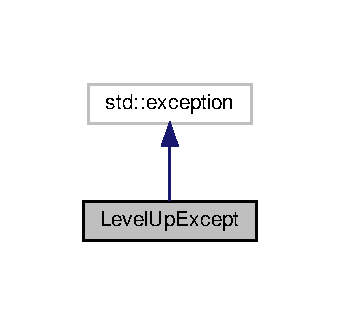
\includegraphics[width=163pt]{classLevelUpExcept__inherit__graph}
\end{center}
\end{figure}


Collaboration diagram for Level\+Up\+Except\+:
\nopagebreak
\begin{figure}[H]
\begin{center}
\leavevmode
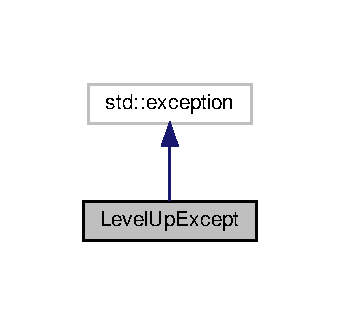
\includegraphics[width=163pt]{classLevelUpExcept__coll__graph}
\end{center}
\end{figure}
\subsection*{Public Member Functions}
\begin{DoxyCompactItemize}
\item 
\mbox{\Hypertarget{classLevelUpExcept_ae885d6dd4fc84fd43f0c834d342a0995}\label{classLevelUpExcept_ae885d6dd4fc84fd43f0c834d342a0995}} 
\hyperlink{classLevelUpExcept_ae885d6dd4fc84fd43f0c834d342a0995}{Level\+Up\+Except} (std\+::string msg)
\begin{DoxyCompactList}\small\item\em Default constructor. \end{DoxyCompactList}\item 
const char $\ast$ \hyperlink{classLevelUpExcept_a4a4cacd5c4f9ee0a691a57dd231d7c46}{what} () const noexcept override
\begin{DoxyCompactList}\small\item\em Throw function. \end{DoxyCompactList}\end{DoxyCompactItemize}


\subsection{Member Function Documentation}
\mbox{\Hypertarget{classLevelUpExcept_a4a4cacd5c4f9ee0a691a57dd231d7c46}\label{classLevelUpExcept_a4a4cacd5c4f9ee0a691a57dd231d7c46}} 
\index{Level\+Up\+Except@{Level\+Up\+Except}!what@{what}}
\index{what@{what}!Level\+Up\+Except@{Level\+Up\+Except}}
\subsubsection{\texorpdfstring{what()}{what()}}
{\footnotesize\ttfamily const char$\ast$ Level\+Up\+Except\+::what (\begin{DoxyParamCaption}{ }\end{DoxyParamCaption}) const\hspace{0.3cm}{\ttfamily [inline]}, {\ttfamily [override]}, {\ttfamily [noexcept]}}



Throw function. 

\begin{DoxyReturn}{Returns}
C-\/string with error message 
\end{DoxyReturn}


The documentation for this class was generated from the following file\+:\begin{DoxyCompactItemize}
\item 
include/Level\+Up.\+h\end{DoxyCompactItemize}

\hypertarget{classLLExcept}{}\section{L\+L\+Except Class Reference}
\label{classLLExcept}\index{L\+L\+Except@{L\+L\+Except}}


This class is used for LL parser exceptions.  




{\ttfamily \#include $<$L\+L\+Parser.\+h$>$}



Inheritance diagram for L\+L\+Except\+:
\nopagebreak
\begin{figure}[H]
\begin{center}
\leavevmode
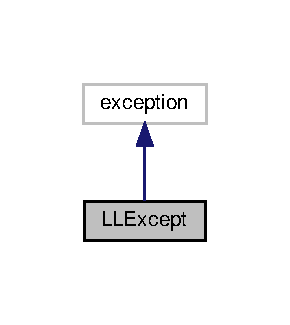
\includegraphics[width=139pt]{classLLExcept__inherit__graph}
\end{center}
\end{figure}


Collaboration diagram for L\+L\+Except\+:
\nopagebreak
\begin{figure}[H]
\begin{center}
\leavevmode
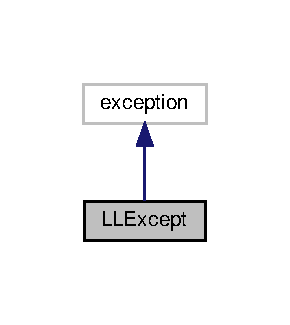
\includegraphics[width=139pt]{classLLExcept__coll__graph}
\end{center}
\end{figure}
\subsection*{Public Member Functions}
\begin{DoxyCompactItemize}
\item 
\mbox{\Hypertarget{classLLExcept_a7ba6f4350aa309e310a67ba732e5c802}\label{classLLExcept_a7ba6f4350aa309e310a67ba732e5c802}} 
\hyperlink{classLLExcept_a7ba6f4350aa309e310a67ba732e5c802}{L\+L\+Except} (std\+::string msg)
\begin{DoxyCompactList}\small\item\em Constructor for LL exception taking its error message as argument. \end{DoxyCompactList}\item 
const char $\ast$ \hyperlink{classLLExcept_a15bcfc8d70217d9532280cf419ee7fa9}{what} () const noexcept override
\begin{DoxyCompactList}\small\item\em Throw function. \end{DoxyCompactList}\end{DoxyCompactItemize}


\subsection{Detailed Description}
This class is used for LL parser exceptions. 

\subsection{Member Function Documentation}
\mbox{\Hypertarget{classLLExcept_a15bcfc8d70217d9532280cf419ee7fa9}\label{classLLExcept_a15bcfc8d70217d9532280cf419ee7fa9}} 
\index{L\+L\+Except@{L\+L\+Except}!what@{what}}
\index{what@{what}!L\+L\+Except@{L\+L\+Except}}
\subsubsection{\texorpdfstring{what()}{what()}}
{\footnotesize\ttfamily const char$\ast$ L\+L\+Except\+::what (\begin{DoxyParamCaption}{ }\end{DoxyParamCaption}) const\hspace{0.3cm}{\ttfamily [inline]}, {\ttfamily [override]}, {\ttfamily [noexcept]}}



Throw function. 

\begin{DoxyReturn}{Returns}
C-\/string with error message 
\end{DoxyReturn}


The documentation for this class was generated from the following file\+:\begin{DoxyCompactItemize}
\item 
include/L\+L\+Parser.\+h\end{DoxyCompactItemize}

\hypertarget{classLLParser}{}\section{L\+L\+Parser Class Reference}
\label{classLLParser}\index{L\+L\+Parser@{L\+L\+Parser}}


This class implements the LL parser functionality.  




{\ttfamily \#include $<$L\+L\+Parser.\+h$>$}

\subsection*{Public Member Functions}
\begin{DoxyCompactItemize}
\item 
\hyperlink{classLLParser_aaa1f2511761d90253b2507a768aebf8a}{L\+L\+Parser} (const \hyperlink{classCFG}{C\+FG} \&cfg, int lookahead)
\begin{DoxyCompactList}\small\item\em Constructor for the LL parser where the cfg is given. \end{DoxyCompactList}\item 
std\+::vector$<$ std\+::string $>$ \hyperlink{classLLParser_a57e0b6627039a37977d17d8b915ee1ea}{parse} (std\+::string input) const
\begin{DoxyCompactList}\small\item\em Function that parses a file with the LL process and returns a vector of actions another function must do. \end{DoxyCompactList}\item 
void \hyperlink{classLLParser_ad56ae17adea4df70ced21f4299dd3429}{parse\+Table\+To\+H\+T\+ML} (std\+::ostream \&on\+Stream) const
\begin{DoxyCompactList}\small\item\em Turns the current parse table into html. \end{DoxyCompactList}\item 
std\+::shared\+\_\+ptr$<$ \hyperlink{classGame}{Game} $>$ \hyperlink{classLLParser_abfc94f8f8cc9230db87183008939dd23}{parse\+File} (const std\+::string \&path) const
\begin{DoxyCompactList}\small\item\em Function that takes a path of a file then streams the whole file to the parse function as a string and returns the parsed file as a game. \end{DoxyCompactList}\end{DoxyCompactItemize}


\subsection{Detailed Description}
This class implements the LL parser functionality. 

\subsection{Constructor \& Destructor Documentation}
\mbox{\Hypertarget{classLLParser_aaa1f2511761d90253b2507a768aebf8a}\label{classLLParser_aaa1f2511761d90253b2507a768aebf8a}} 
\index{L\+L\+Parser@{L\+L\+Parser}!L\+L\+Parser@{L\+L\+Parser}}
\index{L\+L\+Parser@{L\+L\+Parser}!L\+L\+Parser@{L\+L\+Parser}}
\subsubsection{\texorpdfstring{L\+L\+Parser()}{LLParser()}}
{\footnotesize\ttfamily L\+L\+Parser\+::\+L\+L\+Parser (\begin{DoxyParamCaption}\item[{const \hyperlink{classCFG}{C\+FG} \&}]{cfg,  }\item[{int}]{lookahead }\end{DoxyParamCaption})}



Constructor for the LL parser where the cfg is given. 


\begin{DoxyParams}{Parameters}
{\em cfg} & The cfg that is used for the parse table of the LL parser. \\
\hline
\end{DoxyParams}


\subsection{Member Function Documentation}
\mbox{\Hypertarget{classLLParser_a57e0b6627039a37977d17d8b915ee1ea}\label{classLLParser_a57e0b6627039a37977d17d8b915ee1ea}} 
\index{L\+L\+Parser@{L\+L\+Parser}!parse@{parse}}
\index{parse@{parse}!L\+L\+Parser@{L\+L\+Parser}}
\subsubsection{\texorpdfstring{parse()}{parse()}}
{\footnotesize\ttfamily std\+::vector$<$ std\+::string $>$ L\+L\+Parser\+::parse (\begin{DoxyParamCaption}\item[{std\+::string}]{input }\end{DoxyParamCaption}) const}



Function that parses a file with the LL process and returns a vector of actions another function must do. 


\begin{DoxyParams}{Parameters}
{\em input} & The string you are checking. \\
\hline
\end{DoxyParams}
\begin{DoxyReturn}{Returns}
Vector of actions that can be easily parsed to the actual game. 
\end{DoxyReturn}
\mbox{\Hypertarget{classLLParser_abfc94f8f8cc9230db87183008939dd23}\label{classLLParser_abfc94f8f8cc9230db87183008939dd23}} 
\index{L\+L\+Parser@{L\+L\+Parser}!parse\+File@{parse\+File}}
\index{parse\+File@{parse\+File}!L\+L\+Parser@{L\+L\+Parser}}
\subsubsection{\texorpdfstring{parse\+File()}{parseFile()}}
{\footnotesize\ttfamily std\+::shared\+\_\+ptr$<$ \hyperlink{classGame}{Game} $>$ L\+L\+Parser\+::parse\+File (\begin{DoxyParamCaption}\item[{const std\+::string \&}]{path }\end{DoxyParamCaption}) const}



Function that takes a path of a file then streams the whole file to the parse function as a string and returns the parsed file as a game. 


\begin{DoxyParams}{Parameters}
{\em path} & The path of the file. \\
\hline
\end{DoxyParams}
\begin{DoxyReturn}{Returns}
Shared pointer to a fully parsed game. 
\end{DoxyReturn}

\begin{DoxyExceptions}{Exceptions}
{\em \hyperlink{classLLExcept}{L\+L\+Except}} & when a fault happens \\
\hline
\end{DoxyExceptions}
\mbox{\Hypertarget{classLLParser_ad56ae17adea4df70ced21f4299dd3429}\label{classLLParser_ad56ae17adea4df70ced21f4299dd3429}} 
\index{L\+L\+Parser@{L\+L\+Parser}!parse\+Table\+To\+H\+T\+ML@{parse\+Table\+To\+H\+T\+ML}}
\index{parse\+Table\+To\+H\+T\+ML@{parse\+Table\+To\+H\+T\+ML}!L\+L\+Parser@{L\+L\+Parser}}
\subsubsection{\texorpdfstring{parse\+Table\+To\+H\+T\+M\+L()}{parseTableToHTML()}}
{\footnotesize\ttfamily void L\+L\+Parser\+::parse\+Table\+To\+H\+T\+ML (\begin{DoxyParamCaption}\item[{std\+::ostream \&}]{on\+Stream }\end{DoxyParamCaption}) const}



Turns the current parse table into html. 


\begin{DoxyParams}{Parameters}
{\em on\+Stream} & The stream you write to (should be a html file). \\
\hline
\end{DoxyParams}


The documentation for this class was generated from the following files\+:\begin{DoxyCompactItemize}
\item 
include/L\+L\+Parser.\+h\item 
src/L\+L\+Parser.\+cpp\end{DoxyCompactItemize}

\hypertarget{classObject}{}\section{Object Class Reference}
\label{classObject}\index{Object@{Object}}


Inheritance diagram for Object\+:
\nopagebreak
\begin{figure}[H]
\begin{center}
\leavevmode
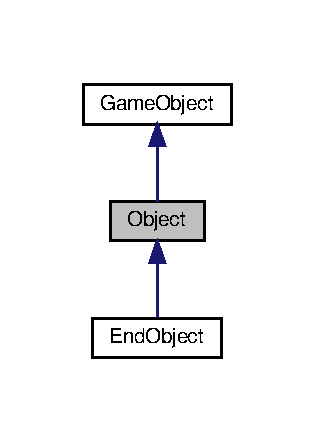
\includegraphics[width=151pt]{classObject__inherit__graph}
\end{center}
\end{figure}


Collaboration diagram for Object\+:
\nopagebreak
\begin{figure}[H]
\begin{center}
\leavevmode
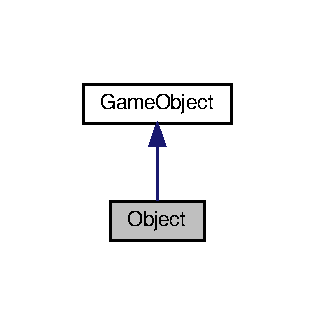
\includegraphics[width=151pt]{classObject__coll__graph}
\end{center}
\end{figure}
\subsection*{Public Member Functions}
\begin{DoxyCompactItemize}
\item 
\mbox{\Hypertarget{classObject_a40860402e64d8008fb42329df7097cdb}\label{classObject_a40860402e64d8008fb42329df7097cdb}} 
\hyperlink{classObject_a40860402e64d8008fb42329df7097cdb}{Object} ()
\begin{DoxyCompactList}\small\item\em Default constructor of object. \end{DoxyCompactList}\item 
\mbox{\Hypertarget{classObject_ab42ffe43dbd5d5cc089493eb60245ee1}\label{classObject_ab42ffe43dbd5d5cc089493eb60245ee1}} 
\hyperlink{classObject_ab42ffe43dbd5d5cc089493eb60245ee1}{$\sim$\+Object} () override=default
\begin{DoxyCompactList}\small\item\em Default Destructor. \end{DoxyCompactList}\item 
void \hyperlink{classObject_a641a0ab489382ba76bd4c538733cc2a4}{set\+Collision} (bool \hyperlink{classObject_aafe6959a6dcbb8c036af3b489386fd98}{can\+Collide})
\begin{DoxyCompactList}\small\item\em Setter for collision of \hyperlink{classObject}{Object}. \end{DoxyCompactList}\item 
void \hyperlink{classObject_a00673d96b2a75c67f9744f9fc1689727}{set\+Location} (const game\+Location \&location)
\begin{DoxyCompactList}\small\item\em Setter for the location of an object. \end{DoxyCompactList}\item 
void \hyperlink{classObject_a0676101219bc31debb04d9d46f64ee15}{set\+Sub\+Objects} (const vector$<$ shared\+\_\+ptr$<$ \hyperlink{classObject}{Object} $>$$>$ \&sub\+Objects)
\begin{DoxyCompactList}\small\item\em Setter for the sub objects of an object. \end{DoxyCompactList}\item 
const vector$<$ shared\+\_\+ptr$<$ \hyperlink{classObject}{Object} $>$ $>$ \& \hyperlink{classObject_afdafb10e24b1025d598d1efbda61c873}{get\+Sub\+Objects} () const
\begin{DoxyCompactList}\small\item\em Getter for the sub objects. \end{DoxyCompactList}\item 
bool \hyperlink{classObject_aafe6959a6dcbb8c036af3b489386fd98}{can\+Collide} () const
\begin{DoxyCompactList}\small\item\em Decides whether an object can be collided with. \end{DoxyCompactList}\item 
const game\+Location \& \hyperlink{classObject_a9a38df5eab9aae1d2706d04528883424}{get\+Location} () const
\begin{DoxyCompactList}\small\item\em Getter for object location. \end{DoxyCompactList}\item 
void \hyperlink{classObject_aa0b8ddc63ff2b6f9a2fd31545e349182}{add\+Sub\+Object} (std\+::shared\+\_\+ptr$<$ \hyperlink{classObject}{Object} $>$ new\+Object)
\begin{DoxyCompactList}\small\item\em Adds a subobject to an object. \end{DoxyCompactList}\end{DoxyCompactItemize}


\subsection{Member Function Documentation}
\mbox{\Hypertarget{classObject_aa0b8ddc63ff2b6f9a2fd31545e349182}\label{classObject_aa0b8ddc63ff2b6f9a2fd31545e349182}} 
\index{Object@{Object}!add\+Sub\+Object@{add\+Sub\+Object}}
\index{add\+Sub\+Object@{add\+Sub\+Object}!Object@{Object}}
\subsubsection{\texorpdfstring{add\+Sub\+Object()}{addSubObject()}}
{\footnotesize\ttfamily void Object\+::add\+Sub\+Object (\begin{DoxyParamCaption}\item[{std\+::shared\+\_\+ptr$<$ \hyperlink{classObject}{Object} $>$}]{new\+Object }\end{DoxyParamCaption})}



Adds a subobject to an object. 


\begin{DoxyParams}{Parameters}
{\em new\+Object} & The subobject to add \\
\hline
\end{DoxyParams}
\mbox{\Hypertarget{classObject_aafe6959a6dcbb8c036af3b489386fd98}\label{classObject_aafe6959a6dcbb8c036af3b489386fd98}} 
\index{Object@{Object}!can\+Collide@{can\+Collide}}
\index{can\+Collide@{can\+Collide}!Object@{Object}}
\subsubsection{\texorpdfstring{can\+Collide()}{canCollide()}}
{\footnotesize\ttfamily bool Object\+::can\+Collide (\begin{DoxyParamCaption}{ }\end{DoxyParamCaption}) const}



Decides whether an object can be collided with. 

\begin{DoxyReturn}{Returns}
True if the object can be collided with 
\end{DoxyReturn}
\mbox{\Hypertarget{classObject_a9a38df5eab9aae1d2706d04528883424}\label{classObject_a9a38df5eab9aae1d2706d04528883424}} 
\index{Object@{Object}!get\+Location@{get\+Location}}
\index{get\+Location@{get\+Location}!Object@{Object}}
\subsubsection{\texorpdfstring{get\+Location()}{getLocation()}}
{\footnotesize\ttfamily const game\+Location \& Object\+::get\+Location (\begin{DoxyParamCaption}{ }\end{DoxyParamCaption}) const}



Getter for object location. 

\begin{DoxyReturn}{Returns}
the gamelocation 
\end{DoxyReturn}
\mbox{\Hypertarget{classObject_afdafb10e24b1025d598d1efbda61c873}\label{classObject_afdafb10e24b1025d598d1efbda61c873}} 
\index{Object@{Object}!get\+Sub\+Objects@{get\+Sub\+Objects}}
\index{get\+Sub\+Objects@{get\+Sub\+Objects}!Object@{Object}}
\subsubsection{\texorpdfstring{get\+Sub\+Objects()}{getSubObjects()}}
{\footnotesize\ttfamily const vector$<$ shared\+\_\+ptr$<$ \hyperlink{classObject}{Object} $>$ $>$ \& Object\+::get\+Sub\+Objects (\begin{DoxyParamCaption}{ }\end{DoxyParamCaption}) const}



Getter for the sub objects. 

\begin{DoxyReturn}{Returns}
Vector with all the sub objects of an object 
\end{DoxyReturn}
\mbox{\Hypertarget{classObject_a641a0ab489382ba76bd4c538733cc2a4}\label{classObject_a641a0ab489382ba76bd4c538733cc2a4}} 
\index{Object@{Object}!set\+Collision@{set\+Collision}}
\index{set\+Collision@{set\+Collision}!Object@{Object}}
\subsubsection{\texorpdfstring{set\+Collision()}{setCollision()}}
{\footnotesize\ttfamily void Object\+::set\+Collision (\begin{DoxyParamCaption}\item[{bool}]{can\+Collide }\end{DoxyParamCaption})}



Setter for collision of \hyperlink{classObject}{Object}. 


\begin{DoxyParams}{Parameters}
{\em can\+Collide} & true if it can collide with other objects \\
\hline
\end{DoxyParams}
\mbox{\Hypertarget{classObject_a00673d96b2a75c67f9744f9fc1689727}\label{classObject_a00673d96b2a75c67f9744f9fc1689727}} 
\index{Object@{Object}!set\+Location@{set\+Location}}
\index{set\+Location@{set\+Location}!Object@{Object}}
\subsubsection{\texorpdfstring{set\+Location()}{setLocation()}}
{\footnotesize\ttfamily void Object\+::set\+Location (\begin{DoxyParamCaption}\item[{const game\+Location \&}]{location }\end{DoxyParamCaption})}



Setter for the location of an object. 


\begin{DoxyParams}{Parameters}
{\em location} & The new location \\
\hline
\end{DoxyParams}
\mbox{\Hypertarget{classObject_a0676101219bc31debb04d9d46f64ee15}\label{classObject_a0676101219bc31debb04d9d46f64ee15}} 
\index{Object@{Object}!set\+Sub\+Objects@{set\+Sub\+Objects}}
\index{set\+Sub\+Objects@{set\+Sub\+Objects}!Object@{Object}}
\subsubsection{\texorpdfstring{set\+Sub\+Objects()}{setSubObjects()}}
{\footnotesize\ttfamily void Object\+::set\+Sub\+Objects (\begin{DoxyParamCaption}\item[{const vector$<$ shared\+\_\+ptr$<$ \hyperlink{classObject}{Object} $>$$>$ \&}]{sub\+Objects }\end{DoxyParamCaption})}



Setter for the sub objects of an object. 


\begin{DoxyParams}{Parameters}
{\em sub\+Objects} & A vector with objects \\
\hline
\end{DoxyParams}


The documentation for this class was generated from the following files\+:\begin{DoxyCompactItemize}
\item 
include/Object.\+h\item 
src/Object.\+cpp\end{DoxyCompactItemize}

\hypertarget{classState}{}\section{State Class Reference}
\label{classState}\index{State@{State}}


Class which represents the state of the Turing machine.  




{\ttfamily \#include $<$Turing\+Machine.\+h$>$}

\subsection*{Public Member Functions}
\begin{DoxyCompactItemize}
\item 
\mbox{\Hypertarget{classState_a95aa2ca390f05627acf00149efd568c7}\label{classState_a95aa2ca390f05627acf00149efd568c7}} 
\hyperlink{classState_a95aa2ca390f05627acf00149efd568c7}{State} ()=default
\begin{DoxyCompactList}\small\item\em Default constructor for a \hyperlink{classState}{State}. \end{DoxyCompactList}\item 
\hyperlink{classState_acec8f151d743a370200a6468cdb6ed5e}{State} (std\+::string name)
\begin{DoxyCompactList}\small\item\em Constructor for state which takes name of state as argument. \end{DoxyCompactList}\item 
\hyperlink{classState_afc0a48251083c35bb1acb67f1fb89f0e}{State} (std\+::string name, std\+::vector$<$ \hyperlink{classTransition}{Transition} $>$ \&\&transitions)
\begin{DoxyCompactList}\small\item\em Constructor for the state which takes the states name and its transitions as arguments. \end{DoxyCompactList}\item 
\mbox{\Hypertarget{classState_a783d52422b544bb226e13de8ecfd6ad6}\label{classState_a783d52422b544bb226e13de8ecfd6ad6}} 
virtual \hyperlink{classState_a783d52422b544bb226e13de8ecfd6ad6}{$\sim$\+State} ()=default
\begin{DoxyCompactList}\small\item\em Default destructor of the \hyperlink{classState}{State}. \end{DoxyCompactList}\item 
void \hyperlink{classState_afa47bb95d7a504a74d0cd9f5deb6893b}{add\+\_\+transition} (\hyperlink{classTransition}{Transition} \&\&transition)
\begin{DoxyCompactList}\small\item\em Adds a transition to the state. \end{DoxyCompactList}\item 
std\+::string \hyperlink{classState_ab732c53a7478c2a24217283340e0c165}{get\+\_\+name} () const
\begin{DoxyCompactList}\small\item\em Getter for the name of the state. \end{DoxyCompactList}\item 
const std\+::vector$<$ \hyperlink{classTransition}{Transition} $>$ \hyperlink{classState_a652bb5b393761ec2d42445f96446c4a6}{get\+\_\+transitions} () const
\begin{DoxyCompactList}\small\item\em Getter for the transitions of the state. \end{DoxyCompactList}\item 
const \hyperlink{classTransition}{Transition} $\ast$ \hyperlink{classState_a807d7c8ed8b9c093d91900217dd302c1}{find\+\_\+transition} (std\+::vector$<$ \hyperlink{classTapeSymbol}{Tape\+Symbol} $\ast$ $>$ \&input) const
\begin{DoxyCompactList}\small\item\em This functions searches for the transition with a certain input If none is found, this function returns a nullptr. \end{DoxyCompactList}\item 
bool \hyperlink{classState_ab98d310aaceb21737346521c5bc6fc6c}{operator==} (const \hyperlink{classState}{State} \&other) const
\begin{DoxyCompactList}\small\item\em Equality operator for \hyperlink{classState}{State}. \end{DoxyCompactList}\end{DoxyCompactItemize}


\subsection{Detailed Description}
Class which represents the state of the Turing machine. 

\subsection{Constructor \& Destructor Documentation}
\mbox{\Hypertarget{classState_acec8f151d743a370200a6468cdb6ed5e}\label{classState_acec8f151d743a370200a6468cdb6ed5e}} 
\index{State@{State}!State@{State}}
\index{State@{State}!State@{State}}
\subsubsection{\texorpdfstring{State()}{State()}\hspace{0.1cm}{\footnotesize\ttfamily [1/2]}}
{\footnotesize\ttfamily State\+::\+State (\begin{DoxyParamCaption}\item[{std\+::string}]{name }\end{DoxyParamCaption})\hspace{0.3cm}{\ttfamily [explicit]}}



Constructor for state which takes name of state as argument. 


\begin{DoxyParams}{Parameters}
{\em name} & Name of the state \\
\hline
\end{DoxyParams}
\mbox{\Hypertarget{classState_afc0a48251083c35bb1acb67f1fb89f0e}\label{classState_afc0a48251083c35bb1acb67f1fb89f0e}} 
\index{State@{State}!State@{State}}
\index{State@{State}!State@{State}}
\subsubsection{\texorpdfstring{State()}{State()}\hspace{0.1cm}{\footnotesize\ttfamily [2/2]}}
{\footnotesize\ttfamily State\+::\+State (\begin{DoxyParamCaption}\item[{std\+::string}]{name,  }\item[{std\+::vector$<$ \hyperlink{classTransition}{Transition} $>$ \&\&}]{transitions }\end{DoxyParamCaption})}



Constructor for the state which takes the states name and its transitions as arguments. 


\begin{DoxyParams}{Parameters}
{\em name} & Name of the state \\
\hline
{\em transitions} & Transitions of the state \\
\hline
\end{DoxyParams}


\subsection{Member Function Documentation}
\mbox{\Hypertarget{classState_afa47bb95d7a504a74d0cd9f5deb6893b}\label{classState_afa47bb95d7a504a74d0cd9f5deb6893b}} 
\index{State@{State}!add\+\_\+transition@{add\+\_\+transition}}
\index{add\+\_\+transition@{add\+\_\+transition}!State@{State}}
\subsubsection{\texorpdfstring{add\+\_\+transition()}{add\_transition()}}
{\footnotesize\ttfamily void State\+::add\+\_\+transition (\begin{DoxyParamCaption}\item[{\hyperlink{classTransition}{Transition} \&\&}]{transition }\end{DoxyParamCaption})}



Adds a transition to the state. 


\begin{DoxyParams}{Parameters}
{\em transition} & \hyperlink{classTransition}{Transition} to add to the state \\
\hline
\end{DoxyParams}
\mbox{\Hypertarget{classState_a807d7c8ed8b9c093d91900217dd302c1}\label{classState_a807d7c8ed8b9c093d91900217dd302c1}} 
\index{State@{State}!find\+\_\+transition@{find\+\_\+transition}}
\index{find\+\_\+transition@{find\+\_\+transition}!State@{State}}
\subsubsection{\texorpdfstring{find\+\_\+transition()}{find\_transition()}}
{\footnotesize\ttfamily const \hyperlink{classTransition}{Transition} $\ast$ State\+::find\+\_\+transition (\begin{DoxyParamCaption}\item[{std\+::vector$<$ \hyperlink{classTapeSymbol}{Tape\+Symbol} $\ast$ $>$ \&}]{input }\end{DoxyParamCaption}) const}



This functions searches for the transition with a certain input If none is found, this function returns a nullptr. 


\begin{DoxyParams}{Parameters}
{\em input} & Input to search for \\
\hline
\end{DoxyParams}
\begin{DoxyReturn}{Returns}
Pointer to transitions 
\end{DoxyReturn}
\mbox{\Hypertarget{classState_ab732c53a7478c2a24217283340e0c165}\label{classState_ab732c53a7478c2a24217283340e0c165}} 
\index{State@{State}!get\+\_\+name@{get\+\_\+name}}
\index{get\+\_\+name@{get\+\_\+name}!State@{State}}
\subsubsection{\texorpdfstring{get\+\_\+name()}{get\_name()}}
{\footnotesize\ttfamily std\+::string State\+::get\+\_\+name (\begin{DoxyParamCaption}{ }\end{DoxyParamCaption}) const}



Getter for the name of the state. 

\begin{DoxyReturn}{Returns}
Name of the state 
\end{DoxyReturn}
\mbox{\Hypertarget{classState_a652bb5b393761ec2d42445f96446c4a6}\label{classState_a652bb5b393761ec2d42445f96446c4a6}} 
\index{State@{State}!get\+\_\+transitions@{get\+\_\+transitions}}
\index{get\+\_\+transitions@{get\+\_\+transitions}!State@{State}}
\subsubsection{\texorpdfstring{get\+\_\+transitions()}{get\_transitions()}}
{\footnotesize\ttfamily const std\+::vector$<$ \hyperlink{classTransition}{Transition} $>$ State\+::get\+\_\+transitions (\begin{DoxyParamCaption}{ }\end{DoxyParamCaption}) const}



Getter for the transitions of the state. 

\begin{DoxyReturn}{Returns}
Transitions of the state 
\end{DoxyReturn}
\mbox{\Hypertarget{classState_ab98d310aaceb21737346521c5bc6fc6c}\label{classState_ab98d310aaceb21737346521c5bc6fc6c}} 
\index{State@{State}!operator==@{operator==}}
\index{operator==@{operator==}!State@{State}}
\subsubsection{\texorpdfstring{operator==()}{operator==()}}
{\footnotesize\ttfamily bool State\+::operator== (\begin{DoxyParamCaption}\item[{const \hyperlink{classState}{State} \&}]{other }\end{DoxyParamCaption}) const}



Equality operator for \hyperlink{classState}{State}. 


\begin{DoxyParams}{Parameters}
{\em other} & \hyperlink{classState}{State} to compare with \\
\hline
\end{DoxyParams}
\begin{DoxyReturn}{Returns}
True if this \hyperlink{classState}{State} is equal to the other 
\end{DoxyReturn}


The documentation for this class was generated from the following files\+:\begin{DoxyCompactItemize}
\item 
include/Turing\+Machine.\+h\item 
src/Turing\+Machine.\+cpp\end{DoxyCompactItemize}

\hypertarget{classTapeSymbol}{}\section{Tape\+Symbol Class Reference}
\label{classTapeSymbol}\index{Tape\+Symbol@{Tape\+Symbol}}


This class represents a tape symbol of a Turing machine.  




{\ttfamily \#include $<$Turing\+Machine.\+h$>$}

\subsection*{Public Member Functions}
\begin{DoxyCompactItemize}
\item 
\mbox{\Hypertarget{classTapeSymbol_a8b667065ca9dbb1840b6e5b940069214}\label{classTapeSymbol_a8b667065ca9dbb1840b6e5b940069214}} 
\hyperlink{classTapeSymbol_a8b667065ca9dbb1840b6e5b940069214}{Tape\+Symbol} ()=default
\begin{DoxyCompactList}\small\item\em Default constructor of Tape Symbol. \end{DoxyCompactList}\item 
\hyperlink{classTapeSymbol_ac4babc556460fd8d7da09115d9b19076}{Tape\+Symbol} (std\+::string \&value)
\begin{DoxyCompactList}\small\item\em Constructor for tape symbol which takes its value as input. \end{DoxyCompactList}\item 
\mbox{\Hypertarget{classTapeSymbol_aa0474beea062da16777821736c788835}\label{classTapeSymbol_aa0474beea062da16777821736c788835}} 
\hyperlink{classTapeSymbol_aa0474beea062da16777821736c788835}{$\sim$\+Tape\+Symbol} ()=default
\begin{DoxyCompactList}\small\item\em Default destructor of the Tape Symbol. \end{DoxyCompactList}\item 
std\+::string \hyperlink{classTapeSymbol_a4f995f73db8026a4511cac0e7da6b66a}{get\+\_\+value\+\_\+string} () const
\begin{DoxyCompactList}\small\item\em Function that returns the value of the tape symbol. \end{DoxyCompactList}\item 
bool \hyperlink{classTapeSymbol_a4b36c3f7a3631d02d77c1eb2efa063a0}{operator==} (\hyperlink{classTapeSymbol}{Tape\+Symbol} \&other) const
\begin{DoxyCompactList}\small\item\em Equality operator for \hyperlink{classTapeSymbol}{Tape\+Symbol}. \end{DoxyCompactList}\end{DoxyCompactItemize}


\subsection{Detailed Description}
This class represents a tape symbol of a Turing machine. 

\subsection{Constructor \& Destructor Documentation}
\mbox{\Hypertarget{classTapeSymbol_ac4babc556460fd8d7da09115d9b19076}\label{classTapeSymbol_ac4babc556460fd8d7da09115d9b19076}} 
\index{Tape\+Symbol@{Tape\+Symbol}!Tape\+Symbol@{Tape\+Symbol}}
\index{Tape\+Symbol@{Tape\+Symbol}!Tape\+Symbol@{Tape\+Symbol}}
\subsubsection{\texorpdfstring{Tape\+Symbol()}{TapeSymbol()}}
{\footnotesize\ttfamily Tape\+Symbol\+::\+Tape\+Symbol (\begin{DoxyParamCaption}\item[{std\+::string \&}]{value }\end{DoxyParamCaption})\hspace{0.3cm}{\ttfamily [explicit]}}



Constructor for tape symbol which takes its value as input. 


\begin{DoxyParams}{Parameters}
{\em value} & Value of the tape symbol \\
\hline
\end{DoxyParams}


\subsection{Member Function Documentation}
\mbox{\Hypertarget{classTapeSymbol_a4f995f73db8026a4511cac0e7da6b66a}\label{classTapeSymbol_a4f995f73db8026a4511cac0e7da6b66a}} 
\index{Tape\+Symbol@{Tape\+Symbol}!get\+\_\+value\+\_\+string@{get\+\_\+value\+\_\+string}}
\index{get\+\_\+value\+\_\+string@{get\+\_\+value\+\_\+string}!Tape\+Symbol@{Tape\+Symbol}}
\subsubsection{\texorpdfstring{get\+\_\+value\+\_\+string()}{get\_value\_string()}}
{\footnotesize\ttfamily std\+::string Tape\+Symbol\+::get\+\_\+value\+\_\+string (\begin{DoxyParamCaption}{ }\end{DoxyParamCaption}) const}



Function that returns the value of the tape symbol. 

\begin{DoxyReturn}{Returns}
the value as a string. 
\end{DoxyReturn}
\mbox{\Hypertarget{classTapeSymbol_a4b36c3f7a3631d02d77c1eb2efa063a0}\label{classTapeSymbol_a4b36c3f7a3631d02d77c1eb2efa063a0}} 
\index{Tape\+Symbol@{Tape\+Symbol}!operator==@{operator==}}
\index{operator==@{operator==}!Tape\+Symbol@{Tape\+Symbol}}
\subsubsection{\texorpdfstring{operator==()}{operator==()}}
{\footnotesize\ttfamily bool Tape\+Symbol\+::operator== (\begin{DoxyParamCaption}\item[{\hyperlink{classTapeSymbol}{Tape\+Symbol} \&}]{other }\end{DoxyParamCaption}) const}



Equality operator for \hyperlink{classTapeSymbol}{Tape\+Symbol}. 


\begin{DoxyParams}{Parameters}
{\em other} & Other tape symbol \\
\hline
\end{DoxyParams}
\begin{DoxyReturn}{Returns}
True if this Tape Symbol is equal to the other one 
\end{DoxyReturn}


The documentation for this class was generated from the following files\+:\begin{DoxyCompactItemize}
\item 
include/Turing\+Machine.\+h\item 
src/Turing\+Machine.\+cpp\end{DoxyCompactItemize}

\hypertarget{classTransition}{}\section{Transition Class Reference}
\label{classTransition}\index{Transition@{Transition}}


Class which represents a Turing machine transition.  




{\ttfamily \#include $<$Turing\+Machine.\+h$>$}

\subsection*{Public Member Functions}
\begin{DoxyCompactItemize}
\item 
\hyperlink{classTransition_af32acfec1e8d6b27dee2634e538731f3}{Transition} (\hyperlink{classState}{State} $\ast$to, std\+::vector$<$ \hyperlink{classTapeSymbol}{Tape\+Symbol} $\ast$ $>$ \&\&input, std\+::vector$<$ \hyperlink{classTapeSymbol}{Tape\+Symbol} $\ast$ $>$ \&\&write, std\+::vector$<$ Direction $>$ \&\&directions)
\begin{DoxyCompactList}\small\item\em Constructor for transition. \end{DoxyCompactList}\item 
const std\+::vector$<$ \hyperlink{classTapeSymbol}{Tape\+Symbol} $\ast$$>$ \hyperlink{classTransition_ab7c192c99fa344b7c629b7a570ae148e}{get\+\_\+input\+\_\+symbols} () const
\begin{DoxyCompactList}\small\item\em Getter for input symbols. \end{DoxyCompactList}\item 
const \hyperlink{classState}{State} $\ast$ \hyperlink{classTransition_ae355340b9b802d1783fe3d596e9f1f6d}{get\+\_\+next\+\_\+state} () const
\begin{DoxyCompactList}\small\item\em Getter for the next state. \end{DoxyCompactList}\item 
std\+::vector$<$ \hyperlink{classTapeSymbol}{Tape\+Symbol} $\ast$ $>$ \hyperlink{classTransition_a313ac6ed2730925df3c79eb2ad0ca2b8}{get\+\_\+write\+\_\+symbols} () const
\begin{DoxyCompactList}\small\item\em Getter for the write symbols. \end{DoxyCompactList}\item 
std\+::vector$<$ Direction $>$ \hyperlink{classTransition_a0d4ad2ca5300f0ff1ef6d57f0d40c0f8}{get\+\_\+direction} () const
\begin{DoxyCompactList}\small\item\em Getter for the direction of the \hyperlink{classTransition}{Transition}. \end{DoxyCompactList}\end{DoxyCompactItemize}


\subsection{Detailed Description}
Class which represents a Turing machine transition. 

\subsection{Constructor \& Destructor Documentation}
\mbox{\Hypertarget{classTransition_af32acfec1e8d6b27dee2634e538731f3}\label{classTransition_af32acfec1e8d6b27dee2634e538731f3}} 
\index{Transition@{Transition}!Transition@{Transition}}
\index{Transition@{Transition}!Transition@{Transition}}
\subsubsection{\texorpdfstring{Transition()}{Transition()}}
{\footnotesize\ttfamily Transition\+::\+Transition (\begin{DoxyParamCaption}\item[{\hyperlink{classState}{State} $\ast$}]{to,  }\item[{std\+::vector$<$ \hyperlink{classTapeSymbol}{Tape\+Symbol} $\ast$ $>$ \&\&}]{input,  }\item[{std\+::vector$<$ \hyperlink{classTapeSymbol}{Tape\+Symbol} $\ast$ $>$ \&\&}]{write,  }\item[{std\+::vector$<$ Direction $>$ \&\&}]{directions }\end{DoxyParamCaption})}



Constructor for transition. 


\begin{DoxyParams}{Parameters}
{\em from} & state from where the finite control starts \\
\hline
{\em to} & state to where the finite control goes \\
\hline
{\em input} & inputsymbol to trigger this transition \\
\hline
{\em write} & tapesymbol to write on the tape \\
\hline
{\em direction} & direction of the head movement for this transition \\
\hline
\end{DoxyParams}


\subsection{Member Function Documentation}
\mbox{\Hypertarget{classTransition_a0d4ad2ca5300f0ff1ef6d57f0d40c0f8}\label{classTransition_a0d4ad2ca5300f0ff1ef6d57f0d40c0f8}} 
\index{Transition@{Transition}!get\+\_\+direction@{get\+\_\+direction}}
\index{get\+\_\+direction@{get\+\_\+direction}!Transition@{Transition}}
\subsubsection{\texorpdfstring{get\+\_\+direction()}{get\_direction()}}
{\footnotesize\ttfamily std\+::vector$<$ Direction $>$ Transition\+::get\+\_\+direction (\begin{DoxyParamCaption}{ }\end{DoxyParamCaption}) const}



Getter for the direction of the \hyperlink{classTransition}{Transition}. 

\begin{DoxyReturn}{Returns}
Directions of the \hyperlink{classTransition}{Transition} 
\end{DoxyReturn}
\mbox{\Hypertarget{classTransition_ab7c192c99fa344b7c629b7a570ae148e}\label{classTransition_ab7c192c99fa344b7c629b7a570ae148e}} 
\index{Transition@{Transition}!get\+\_\+input\+\_\+symbols@{get\+\_\+input\+\_\+symbols}}
\index{get\+\_\+input\+\_\+symbols@{get\+\_\+input\+\_\+symbols}!Transition@{Transition}}
\subsubsection{\texorpdfstring{get\+\_\+input\+\_\+symbols()}{get\_input\_symbols()}}
{\footnotesize\ttfamily const std\+::vector$<$ \hyperlink{classTapeSymbol}{Tape\+Symbol} $\ast$ $>$ Transition\+::get\+\_\+input\+\_\+symbols (\begin{DoxyParamCaption}{ }\end{DoxyParamCaption}) const}



Getter for input symbols. 

\begin{DoxyReturn}{Returns}
Vector of input symbols 
\end{DoxyReturn}
\mbox{\Hypertarget{classTransition_ae355340b9b802d1783fe3d596e9f1f6d}\label{classTransition_ae355340b9b802d1783fe3d596e9f1f6d}} 
\index{Transition@{Transition}!get\+\_\+next\+\_\+state@{get\+\_\+next\+\_\+state}}
\index{get\+\_\+next\+\_\+state@{get\+\_\+next\+\_\+state}!Transition@{Transition}}
\subsubsection{\texorpdfstring{get\+\_\+next\+\_\+state()}{get\_next\_state()}}
{\footnotesize\ttfamily const \hyperlink{classState}{State} $\ast$ Transition\+::get\+\_\+next\+\_\+state (\begin{DoxyParamCaption}{ }\end{DoxyParamCaption}) const}



Getter for the next state. 

\begin{DoxyReturn}{Returns}
Pointer to the next state 
\end{DoxyReturn}
\mbox{\Hypertarget{classTransition_a313ac6ed2730925df3c79eb2ad0ca2b8}\label{classTransition_a313ac6ed2730925df3c79eb2ad0ca2b8}} 
\index{Transition@{Transition}!get\+\_\+write\+\_\+symbols@{get\+\_\+write\+\_\+symbols}}
\index{get\+\_\+write\+\_\+symbols@{get\+\_\+write\+\_\+symbols}!Transition@{Transition}}
\subsubsection{\texorpdfstring{get\+\_\+write\+\_\+symbols()}{get\_write\_symbols()}}
{\footnotesize\ttfamily std\+::vector$<$ \hyperlink{classTapeSymbol}{Tape\+Symbol} $\ast$ $>$ Transition\+::get\+\_\+write\+\_\+symbols (\begin{DoxyParamCaption}{ }\end{DoxyParamCaption}) const}



Getter for the write symbols. 

\begin{DoxyReturn}{Returns}
Vector of write symbols 
\end{DoxyReturn}


The documentation for this class was generated from the following files\+:\begin{DoxyCompactItemize}
\item 
include/Turing\+Machine.\+h\item 
src/Turing\+Machine.\+cpp\end{DoxyCompactItemize}

\hypertarget{classTuringMachine}{}\section{Turing\+Machine Class Reference}
\label{classTuringMachine}\index{Turing\+Machine@{Turing\+Machine}}


This class represents a Turing machine.  




{\ttfamily \#include $<$Turing\+Machine.\+h$>$}

\subsection*{Public Member Functions}
\begin{DoxyCompactItemize}
\item 
\mbox{\Hypertarget{classTuringMachine_ab998b1ffcadd9e6101707346749ecd53}\label{classTuringMachine_ab998b1ffcadd9e6101707346749ecd53}} 
\hyperlink{classTuringMachine_ab998b1ffcadd9e6101707346749ecd53}{Turing\+Machine} ()=default
\begin{DoxyCompactList}\small\item\em Default constructor of Turing machine. \end{DoxyCompactList}\item 
\hyperlink{classTuringMachine_abe6ad3a974d2341a75908b0ab6250410}{Turing\+Machine} (std\+::vector$<$ \hyperlink{classState}{State} $\ast$ $>$ \&states, std\+::vector$<$ std\+::string $>$ \&input\+\_\+symbols, std\+::vector$<$ \hyperlink{classTapeSymbol}{Tape\+Symbol} $\ast$ $>$ \&tape\+\_\+symbols, \hyperlink{classState}{State} $\ast$start\+\_\+state, \hyperlink{classTapeSymbol}{Tape\+Symbol} $\ast$blank, std\+::vector$<$ \hyperlink{classState}{State} $\ast$ $>$ \&final\+\_\+states, int amount\+\_\+of\+\_\+tapes)
\begin{DoxyCompactList}\small\item\em Constructor of Turing machine. \end{DoxyCompactList}\item 
\hyperlink{classTuringMachine_ad56c71b24817a917f5e4984035070cc3}{Turing\+Machine} (char input\+\_\+file\mbox{[}$\,$\mbox{]})
\begin{DoxyCompactList}\small\item\em Constructor of Turing machine created from file. \end{DoxyCompactList}\item 
\mbox{\Hypertarget{classTuringMachine_a5279d180cd87e664447c6b40e0ce55e2}\label{classTuringMachine_a5279d180cd87e664447c6b40e0ce55e2}} 
\hyperlink{classTuringMachine_a5279d180cd87e664447c6b40e0ce55e2}{$\sim$\+Turing\+Machine} ()
\begin{DoxyCompactList}\small\item\em Destructor for Turing machine. \end{DoxyCompactList}\item 
bool \hyperlink{classTuringMachine_a6ac17dcb3bce76b6e02154cb749526c4}{evaluate\+\_\+string} ()
\begin{DoxyCompactList}\small\item\em Evaluates a string using the Turing machine Important\+: the tapes need to be initialized first (setup\+\_\+tapes) \end{DoxyCompactList}\item 
std\+::vector$<$ std\+::string $>$ \hyperlink{classTuringMachine_a103fa5e9b267ea625770297cb9168a34}{calculate} ()
\begin{DoxyCompactList}\small\item\em This function does a calculation with the Turing machine Important\+:the tapes need to be initialized first (setup\+\_\+tapes) \end{DoxyCompactList}\item 
void \hyperlink{classTuringMachine_add19f4c90678b56d5a78d0e88c389cd8}{setup\+\_\+tapes\+\_\+with\+\_\+string} (std\+::vector$<$ std\+::string $>$ \&input)
\begin{DoxyCompactList}\small\item\em Setup the tapes with a certain input. \end{DoxyCompactList}\item 
\mbox{\Hypertarget{classTuringMachine_a6423abd83f107001747c544fbd111be3}\label{classTuringMachine_a6423abd83f107001747c544fbd111be3}} 
void \hyperlink{classTuringMachine_a6423abd83f107001747c544fbd111be3}{reset\+\_\+tapes} ()
\begin{DoxyCompactList}\small\item\em Resets the tapes of the Turing machine. \end{DoxyCompactList}\item 
void \hyperlink{classTuringMachine_a15485e4e3a38f21581f0d13127b6e6f7}{add\+\_\+subroutine} (\hyperlink{classTuringMachine}{Turing\+Machine} \&\&subroutine, \hyperlink{classState}{State} $\ast$state\+From, std\+::vector$<$ \hyperlink{classTapeSymbol}{Tape\+Symbol} $\ast$$>$ \&\&get\+In\+\_\+read, std\+::vector$<$ \hyperlink{classTapeSymbol}{Tape\+Symbol} $\ast$$>$ \&\&get\+In\+\_\+write, std\+::vector$<$ Direction $>$ \&\&get\+In\+\_\+dir, \hyperlink{classState}{State} $\ast$state\+To, std\+::vector$<$ \hyperlink{classTapeSymbol}{Tape\+Symbol} $\ast$$>$ \&\&get\+Out\+\_\+read, std\+::vector$<$ \hyperlink{classTapeSymbol}{Tape\+Symbol} $\ast$$>$ \&\&get\+Out\+\_\+write, std\+::vector$<$ Direction $>$ \&\&get\+Out\+\_\+dir)
\begin{DoxyCompactList}\small\item\em Adds a subroutine to the Turing machine. \end{DoxyCompactList}\item 
void \hyperlink{classTuringMachine_abd6288a60955a8b1b2d0f58d0b3d63da}{to\+\_\+dot} (std\+::ostream \&os)
\begin{DoxyCompactList}\small\item\em Generate a dot file of the Turing machine. \end{DoxyCompactList}\item 
const \hyperlink{classState}{State} $\ast$ \hyperlink{classTuringMachine_a596149a33ff6f9c49100c71977ad16c6}{get\+\_\+start\+\_\+state} ()
\begin{DoxyCompactList}\small\item\em Getter for start \hyperlink{classState}{State}. \end{DoxyCompactList}\item 
const std\+::vector$<$ \hyperlink{classState}{State} $\ast$ $>$ \& \hyperlink{classTuringMachine_ab34c3253e9d158d91a8d2e4473267761}{get\+\_\+final\+\_\+states} ()
\begin{DoxyCompactList}\small\item\em Getter for the final states of the Turing machine. \end{DoxyCompactList}\end{DoxyCompactItemize}


\subsection{Detailed Description}
This class represents a Turing machine. 

\subsection{Constructor \& Destructor Documentation}
\mbox{\Hypertarget{classTuringMachine_abe6ad3a974d2341a75908b0ab6250410}\label{classTuringMachine_abe6ad3a974d2341a75908b0ab6250410}} 
\index{Turing\+Machine@{Turing\+Machine}!Turing\+Machine@{Turing\+Machine}}
\index{Turing\+Machine@{Turing\+Machine}!Turing\+Machine@{Turing\+Machine}}
\subsubsection{\texorpdfstring{Turing\+Machine()}{TuringMachine()}\hspace{0.1cm}{\footnotesize\ttfamily [1/2]}}
{\footnotesize\ttfamily Turing\+Machine\+::\+Turing\+Machine (\begin{DoxyParamCaption}\item[{std\+::vector$<$ \hyperlink{classState}{State} $\ast$ $>$ \&}]{states,  }\item[{std\+::vector$<$ std\+::string $>$ \&}]{input\+\_\+symbols,  }\item[{std\+::vector$<$ \hyperlink{classTapeSymbol}{Tape\+Symbol} $\ast$ $>$ \&}]{tape\+\_\+symbols,  }\item[{\hyperlink{classState}{State} $\ast$}]{start\+\_\+state,  }\item[{\hyperlink{classTapeSymbol}{Tape\+Symbol} $\ast$}]{blank,  }\item[{std\+::vector$<$ \hyperlink{classState}{State} $\ast$ $>$ \&}]{final\+\_\+states,  }\item[{int}]{amount\+\_\+of\+\_\+tapes }\end{DoxyParamCaption})}



Constructor of Turing machine. 


\begin{DoxyParams}{Parameters}
{\em states} & States of Turing machine \\
\hline
{\em input\+\_\+symbols} & Input symbols op Turing machine \\
\hline
{\em tape\+\_\+symbols} & Tape symbols of Turing machine \\
\hline
{\em start\+\_\+state} & Start state of Turing machine \\
\hline
{\em blank} & Blank symbol of Turing machine \\
\hline
{\em final\+\_\+states} & Final states of Turing machine \\
\hline
{\em amount\+\_\+of\+\_\+tapes} & The amount of tapes of a Turing machine (multi tape support) \\
\hline
\end{DoxyParams}
\mbox{\Hypertarget{classTuringMachine_ad56c71b24817a917f5e4984035070cc3}\label{classTuringMachine_ad56c71b24817a917f5e4984035070cc3}} 
\index{Turing\+Machine@{Turing\+Machine}!Turing\+Machine@{Turing\+Machine}}
\index{Turing\+Machine@{Turing\+Machine}!Turing\+Machine@{Turing\+Machine}}
\subsubsection{\texorpdfstring{Turing\+Machine()}{TuringMachine()}\hspace{0.1cm}{\footnotesize\ttfamily [2/2]}}
{\footnotesize\ttfamily Turing\+Machine\+::\+Turing\+Machine (\begin{DoxyParamCaption}\item[{char}]{input\+\_\+file\mbox{[}$\,$\mbox{]} }\end{DoxyParamCaption})\hspace{0.3cm}{\ttfamily [explicit]}}



Constructor of Turing machine created from file. 


\begin{DoxyParams}{Parameters}
{\em input\+\_\+file} & Input file in json \\
\hline
\end{DoxyParams}


\subsection{Member Function Documentation}
\mbox{\Hypertarget{classTuringMachine_a15485e4e3a38f21581f0d13127b6e6f7}\label{classTuringMachine_a15485e4e3a38f21581f0d13127b6e6f7}} 
\index{Turing\+Machine@{Turing\+Machine}!add\+\_\+subroutine@{add\+\_\+subroutine}}
\index{add\+\_\+subroutine@{add\+\_\+subroutine}!Turing\+Machine@{Turing\+Machine}}
\subsubsection{\texorpdfstring{add\+\_\+subroutine()}{add\_subroutine()}}
{\footnotesize\ttfamily void Turing\+Machine\+::add\+\_\+subroutine (\begin{DoxyParamCaption}\item[{\hyperlink{classTuringMachine}{Turing\+Machine} \&\&}]{subroutine,  }\item[{\hyperlink{classState}{State} $\ast$}]{state\+From,  }\item[{std\+::vector$<$ \hyperlink{classTapeSymbol}{Tape\+Symbol} $\ast$$>$ \&\&}]{get\+In\+\_\+read,  }\item[{std\+::vector$<$ \hyperlink{classTapeSymbol}{Tape\+Symbol} $\ast$$>$ \&\&}]{get\+In\+\_\+write,  }\item[{std\+::vector$<$ Direction $>$ \&\&}]{get\+In\+\_\+dir,  }\item[{\hyperlink{classState}{State} $\ast$}]{state\+To,  }\item[{std\+::vector$<$ \hyperlink{classTapeSymbol}{Tape\+Symbol} $\ast$$>$ \&\&}]{get\+Out\+\_\+read,  }\item[{std\+::vector$<$ \hyperlink{classTapeSymbol}{Tape\+Symbol} $\ast$$>$ \&\&}]{get\+Out\+\_\+write,  }\item[{std\+::vector$<$ Direction $>$ \&\&}]{get\+Out\+\_\+dir }\end{DoxyParamCaption})}



Adds a subroutine to the Turing machine. 


\begin{DoxyParams}{Parameters}
{\em subroutine} & Subroutine to add \\
\hline
{\em state\+From} & From state input \\
\hline
{\em get\+In\+\_\+read} & Read symbols input \\
\hline
{\em get\+In\+\_\+write} & Write symbols input \\
\hline
{\em get\+In\+\_\+dir} & Directions input \\
\hline
{\em state\+To} & To state \\
\hline
{\em get\+Out\+\_\+read} & Read symbols output \\
\hline
{\em get\+Out\+\_\+write} & Write symbols output \\
\hline
{\em get\+Out\+\_\+dir} & Directions output \\
\hline
\end{DoxyParams}
\mbox{\Hypertarget{classTuringMachine_a103fa5e9b267ea625770297cb9168a34}\label{classTuringMachine_a103fa5e9b267ea625770297cb9168a34}} 
\index{Turing\+Machine@{Turing\+Machine}!calculate@{calculate}}
\index{calculate@{calculate}!Turing\+Machine@{Turing\+Machine}}
\subsubsection{\texorpdfstring{calculate()}{calculate()}}
{\footnotesize\ttfamily std\+::vector$<$ std\+::string $>$ Turing\+Machine\+::calculate (\begin{DoxyParamCaption}{ }\end{DoxyParamCaption})}



This function does a calculation with the Turing machine Important\+:the tapes need to be initialized first (setup\+\_\+tapes) 

\begin{DoxyReturn}{Returns}
Vector of strings where the calculation is made on 
\end{DoxyReturn}
\mbox{\Hypertarget{classTuringMachine_a6ac17dcb3bce76b6e02154cb749526c4}\label{classTuringMachine_a6ac17dcb3bce76b6e02154cb749526c4}} 
\index{Turing\+Machine@{Turing\+Machine}!evaluate\+\_\+string@{evaluate\+\_\+string}}
\index{evaluate\+\_\+string@{evaluate\+\_\+string}!Turing\+Machine@{Turing\+Machine}}
\subsubsection{\texorpdfstring{evaluate\+\_\+string()}{evaluate\_string()}}
{\footnotesize\ttfamily bool Turing\+Machine\+::evaluate\+\_\+string (\begin{DoxyParamCaption}{ }\end{DoxyParamCaption})}



Evaluates a string using the Turing machine Important\+: the tapes need to be initialized first (setup\+\_\+tapes) 

\begin{DoxyReturn}{Returns}
True if the string is evaluated by the Turing machine, false if it is not 
\end{DoxyReturn}
\mbox{\Hypertarget{classTuringMachine_ab34c3253e9d158d91a8d2e4473267761}\label{classTuringMachine_ab34c3253e9d158d91a8d2e4473267761}} 
\index{Turing\+Machine@{Turing\+Machine}!get\+\_\+final\+\_\+states@{get\+\_\+final\+\_\+states}}
\index{get\+\_\+final\+\_\+states@{get\+\_\+final\+\_\+states}!Turing\+Machine@{Turing\+Machine}}
\subsubsection{\texorpdfstring{get\+\_\+final\+\_\+states()}{get\_final\_states()}}
{\footnotesize\ttfamily const std\+::vector$<$ \hyperlink{classState}{State} $\ast$ $>$ \& Turing\+Machine\+::get\+\_\+final\+\_\+states (\begin{DoxyParamCaption}{ }\end{DoxyParamCaption})}



Getter for the final states of the Turing machine. 

\begin{DoxyReturn}{Returns}
final states of the Turing machine 
\end{DoxyReturn}
\mbox{\Hypertarget{classTuringMachine_a596149a33ff6f9c49100c71977ad16c6}\label{classTuringMachine_a596149a33ff6f9c49100c71977ad16c6}} 
\index{Turing\+Machine@{Turing\+Machine}!get\+\_\+start\+\_\+state@{get\+\_\+start\+\_\+state}}
\index{get\+\_\+start\+\_\+state@{get\+\_\+start\+\_\+state}!Turing\+Machine@{Turing\+Machine}}
\subsubsection{\texorpdfstring{get\+\_\+start\+\_\+state()}{get\_start\_state()}}
{\footnotesize\ttfamily const \hyperlink{classState}{State} $\ast$ Turing\+Machine\+::get\+\_\+start\+\_\+state (\begin{DoxyParamCaption}{ }\end{DoxyParamCaption})}



Getter for start \hyperlink{classState}{State}. 

\begin{DoxyReturn}{Returns}
start \hyperlink{classState}{State} of Turing machine 
\end{DoxyReturn}
\mbox{\Hypertarget{classTuringMachine_add19f4c90678b56d5a78d0e88c389cd8}\label{classTuringMachine_add19f4c90678b56d5a78d0e88c389cd8}} 
\index{Turing\+Machine@{Turing\+Machine}!setup\+\_\+tapes\+\_\+with\+\_\+string@{setup\+\_\+tapes\+\_\+with\+\_\+string}}
\index{setup\+\_\+tapes\+\_\+with\+\_\+string@{setup\+\_\+tapes\+\_\+with\+\_\+string}!Turing\+Machine@{Turing\+Machine}}
\subsubsection{\texorpdfstring{setup\+\_\+tapes\+\_\+with\+\_\+string()}{setup\_tapes\_with\_string()}}
{\footnotesize\ttfamily void Turing\+Machine\+::setup\+\_\+tapes\+\_\+with\+\_\+string (\begin{DoxyParamCaption}\item[{std\+::vector$<$ std\+::string $>$ \&}]{input }\end{DoxyParamCaption})}



Setup the tapes with a certain input. 


\begin{DoxyParams}{Parameters}
{\em input} & Input the setup the tape with, each string represents a tape \\
\hline
\end{DoxyParams}
\mbox{\Hypertarget{classTuringMachine_abd6288a60955a8b1b2d0f58d0b3d63da}\label{classTuringMachine_abd6288a60955a8b1b2d0f58d0b3d63da}} 
\index{Turing\+Machine@{Turing\+Machine}!to\+\_\+dot@{to\+\_\+dot}}
\index{to\+\_\+dot@{to\+\_\+dot}!Turing\+Machine@{Turing\+Machine}}
\subsubsection{\texorpdfstring{to\+\_\+dot()}{to\_dot()}}
{\footnotesize\ttfamily void Turing\+Machine\+::to\+\_\+dot (\begin{DoxyParamCaption}\item[{std\+::ostream \&}]{os }\end{DoxyParamCaption})}



Generate a dot file of the Turing machine. 


\begin{DoxyParams}{Parameters}
{\em os} & Stream to generate dot file to \\
\hline
\end{DoxyParams}


The documentation for this class was generated from the following files\+:\begin{DoxyCompactItemize}
\item 
include/Turing\+Machine.\+h\item 
src/Turing\+Machine.\+cpp\end{DoxyCompactItemize}

%--- End generated contents ---

% Index
\backmatter
\newpage
\phantomsection
\clearemptydoublepage
\addcontentsline{toc}{chapter}{Index}
\printindex

\end{document}
